%% LyX 2.0.3 created this file.  For more info, see http://www.lyx.org/.
%DIF LATEXDIFF DIFFERENCE FILE
%DIF DEL diff/diffPreamble.tex   Thu Jun 19 10:43:55 2014
%DIF ADD diff/diffPreamble.tex   Thu Jun 19 10:43:55 2014
%% Do not edit unless you really know what you are doing.
\documentclass[12pt,english]{kuthesis}
\usepackage{mathptmx}
\renewcommand{\sfdefault}{lmss}
\renewcommand{\ttdefault}{lmtt}
\usepackage[T1]{fontenc}
\usepackage[utf8]{inputenc}
\usepackage{listings}
\usepackage{geometry}
\geometry{verbose,tmargin=1in,bmargin=1in,lmargin=1in,rmargin=1in}
\setcounter{secnumdepth}{3}
\setcounter{tocdepth}{3}
\usepackage{url}
\usepackage{graphicx}
\usepackage{wrapfig}
\usepackage{setspace}
\usepackage{esint}
\usepackage{hyperref}
\usepackage{xcolor}
\usepackage{easylist}
\usepackage{multirow}
\usepackage{hhline}
\usepackage{lineno}
%\usepackage{mathtools}
%\usepackage[authoryear]{natbib}

\graphicspath{{IntroductionChapter/figures/},{TheoryChapter/figures/}
  ,{DetectorChapter/figures/},{AnalysisChapter/figures/}
  ,{ResultsChapter/figures/},{ConclusionChapter/figures/}
  ,{FutureWorksChapter/figures/},{ZDCRecoChapter/figures/}
  ,{TriggerChapter/figures/},{SystematicsChapter/figures/}}

\newcommand{\JPsi}{J/$\psi$}
\newcommand{\pt}{$p_{T}$}

\doublespacing

\makeatletter

%%%%%%%%%%%%%%%%%%%%%%%%%%%%%% LyX specific LaTeX commands.
\providecommand{\LyX}{L\kern-.1667em\lower.25em\hbox{Y}\kern-.125emX\@}
%% Because html converters don't know tabularnewline
\providecommand{\tabularnewline}{\\}

%%%%%%%%%%%%%%%%%%%%%%%%%%%%%% User specified LaTeX commands.

%used to align decimals in tables according to APA style
\usepackage{dcolumn}
\usepackage{booktabs}

% Set the title and author info
\title{Ultra-peripheral J/$\psi$ production in PbPb collisions at $\sqrt{s_{NN}}$=2.76 TeV with CMS}
\author{R. Patrick Kenny III}


\dept{Department of People who read Abstracts}
\degreetitle{Doctor of Philosophy}
\papertype{Dissertation} %capitalization is important here
\committee{MEMBER 1}{MEMBER 2}{MEMBER 3}{MEMBER 4}{}

\@printd@testrue
\datedefended{October 02, 2012}
\dateapproved{October 03, 2012}

\@ifundefined{showcaptionsetup}{}{%
 \PassOptionsToPackage{caption=false}{subfig}}
\usepackage{subfig}
\makeatother

\usepackage{babel}
%DIF PREAMBLE EXTENSION ADDED BY LATEXDIFF
%DIF UNDERLINE PREAMBLE %DIF PREAMBLE
\RequirePackage[normalem]{ulem} %DIF PREAMBLE
\RequirePackage{color}\definecolor{RED}{rgb}{1,0,0}\definecolor{BLUE}{rgb}{0,0,1} %DIF PREAMBLE
\providecommand{\DIFaddtex}[1]{{\protect\color{blue}\uwave{#1}}} %DIF PREAMBLE
\providecommand{\DIFdeltex}[1]{{\protect\color{red}\sout{#1}}}                      %DIF PREAMBLE
%DIF SAFE PREAMBLE %DIF PREAMBLE
\providecommand{\DIFaddbegin}{} %DIF PREAMBLE
\providecommand{\DIFaddend}{} %DIF PREAMBLE
\providecommand{\DIFdelbegin}{} %DIF PREAMBLE
\providecommand{\DIFdelend}{} %DIF PREAMBLE
%DIF FLOATSAFE PREAMBLE %DIF PREAMBLE
\providecommand{\DIFaddFL}[1]{\DIFadd{#1}} %DIF PREAMBLE
\providecommand{\DIFdelFL}[1]{\DIFdel{#1}} %DIF PREAMBLE
\providecommand{\DIFaddbeginFL}{} %DIF PREAMBLE
\providecommand{\DIFaddendFL}{} %DIF PREAMBLE
\providecommand{\DIFdelbeginFL}{} %DIF PREAMBLE
\providecommand{\DIFdelendFL}{} %DIF PREAMBLE
%DIF END PREAMBLE EXTENSION ADDED BY LATEXDIFF
%DIF PREAMBLE EXTENSION ADDED BY LATEXDIFF
%DIF HYPERREF PREAMBLE %DIF PREAMBLE
\providecommand{\DIFadd}[1]{\texorpdfstring{\DIFaddtex{#1}}{#1}} %DIF PREAMBLE
\providecommand{\DIFdel}[1]{\texorpdfstring{\DIFdeltex{#1}}{}} %DIF PREAMBLE
%DIF END PREAMBLE EXTENSION ADDED BY LATEXDIFF

\begin{document}
  \linenumbers
  \chapter{Introduction}
  \DIFaddbegin \DIFadd{High energy physics probes the smallest scales in order to discover the 
    fundamental constituents of the universe and how they interact.
  From these searches of the smallest scales, the standard model of particle
    physics has emerged. 
  The standard model contains 3 forces, the weak, the electromagnetic, and 
    strong force, and two types of mater that interact through these forces,
    quarks and leptons.
  The quarks can interact through all three forces.
  The leptons however only interact through the weak and electromagnetic force.
  The mater particles interact with each through the three forces by exchanging the
    forces carrying vector bosons. 
  Strong interactions take place by exchange of gluons, the weak by Z$^{0}$ and
    W$^{\pm}$ bosons, and the electromagnetic by photon. 
  }

  \DIFadd{Each of these three forces emerges due to symmetries in the standard model.
  For example, the wave function of the Sch}\"{o}\DIFadd{rdinger equation is comprised
    of complex numbers.
  The standard model does not depend on the phase of these complex numbers. 
  The phases for each of these numbers can be arbitrarily changed at all points
    in space and time without any changing the predictions of the theory.
  This is because the gradient of an arbitrary scaler field can be added to the
    $\vec{A}$, the vector potential, which gives rise to the electromagnetic 
    without changing the magnetic field and electric field that ultimately
    interact with the particles. 
  The invariance of the standard model to the complex phase of the wave 
    function necessitates the existence of the electromagnetic force. 
}

  \DIFadd{The standard model is made of the three such symmetries, each of which is
    described by a gauge group. 
  The U(1) is the group that accounts for the electromagnetic interaction
    and gives rise to the photon. 
  The SU(2) group produces the weak bosons, Z$^{0}$ and W$^{\pm}$.
  The strong force mediated by the gluons are consequence of the SU(3) symmetry
    of the standard model.
  Of these three groups two, SU(2) and SU(3), are non-abelian. 
  The consequence of this, is that the W$^{+}$ and W$^{-}$ can interact with 
    Z$^{0}$ and photon, the gluons can interact with each other. 
  Because the gluons can interact with each other in many more ways that the 
    limited interactions between the W,Z and the photons, the non-abelian 
    nature of the strong force is particularly pronounced. 
}

  \DIFadd{The self-interaction of the gluons produces unique qualities of the strong 
    force: confinement, and asymptotic freedom. 
  }

  \DIFadd{Microseconds after the big bang, the universe existed in a state known as
    the Quark Gluon Plasma (QGP).
  In the QGP, quarks and gluons are not in hadronic bondage, forced to 
    the confines of bound states such as protons and neutrons.
  The Large Hadron Collider (LHC) produces QGP in the lab in PbPb (lead-lead)
    collisions.
  The high energies and rates of the collisions at the LHC make it possible 
    to do detailed studies of the QGP. 
  The LHC is producing rare experimental probes such as suppressed jets and 
    heavy quarkonia at an unprecedented rate in heavy-ion collisions. 
  Physicists now have better constraints on the properties like temperature,
    viscosity, and energy density of the QGP. 
  }\DIFaddend \section{Theoretical Context}
  \section{History }

  \chapter{Photo-nuclear interactions \label{ch:photoNuc}}
    \DIFdelbegin \DIFdel{The }\DIFdelend \DIFaddbegin \DIFadd{In ultra-peripheral heavy-ion collision, the }\DIFaddend colliding nuclei interact \DIFdelbegin \DIFdel{electromagnetically in an ultra-peripheral 
      heavy-ion collision}\DIFdelend \DIFaddbegin \DIFadd{only 
      electromagnetically}\DIFaddend .   
    In such events, no QGP state emerges, and the effects arising from the QGP 
      no longer obscure the initial state effects.
    Other initial state probes such as peripheral nuclear collisions and 
      proton-nucleus collisions have the potential to create the QGP obscuring 
      which effects come from the initial state.
    It is impossible to create the QGP in UPC events because \DIFaddbegin \DIFadd{in UPC events }\DIFaddend the 
      nucleons within the nucleus do not collide. 
    Thus, UPC events provide clarity by enhancing physicists' 
      understanding of the initial state. 

    In particular, these interactions between the field of photons surrounding 
      the colliding nuclei and the gluons within the nuclei can produce a 
      \JPsi{}, probing the gluon density.
    The \JPsi{} can be produced either coherently or incoherently. 
    In the case of coherent interactions, the photon couples to the nucleus 
      as a whole.
    In the incoherent case, the photon couples to the nucleons within the 
      nucleus.
    The UPC \JPsi{} photoproduction cross section is therefore a probe of 
      the initial state of the nucleus.

    This cross section can be calculated using three steps.   
    First, the Weizs\"{a}cker-Williams approximation provides a way to calculate the 
      density of probing photons that surrounds the nucleus. 
    Second, the electron-proton scattering data gives a value for the proton 
      photoproduction cross section at lower energies \DIFaddbegin \DIFadd{\mbox{%DIFAUXCMD
\cite{Klasen:2007pm}
}%DIFAUXCMD
}\DIFaddend .
    Last, a specific model is used to combined the previous two steps in order
      to calculate the nuclear photoproduction cross section. 
    In this thesis the perterbutive Adeluyi and Bertulani (AB), STARlight, and 
      the Leading Twist (LTA) models are discussed. 
    Each of these methods handle the gluon density of the nucleus differently 
      producing a measurable difference in the value of the \JPsi{} 
      photoproduction cross section.
    Measurements at the LHC have provided important constrains to models of the 
      nuclear gluon density.
    The analysis presented in Chapter~\ref{ch:analysis} adds to the existing 
      data in a new kinematic region.
    In this Chapter the theoretical framework for photon-nuclear
      interactions, together with an experimental review of recent results on 
      ultra-peripheral heavy-ion collisions are described. 

  \section{Weizs\"{a}cker-Williams approximation \label{sec:wwAprox}}
    The density of photons surrounding the colliding nuclei can be calculated 
      using the Weizs\"{a}cker-Williams approximation. 
    This approximation relates the electric field of a stationary point charge 
      to the photon field that arises at ultra relativistic velocities. 
    The approximation is semi-classical and combines both classical and quantum 
      elements.
    In the Weizs\"{a}cker-Williams 
      approximation, a Fourier transform of Maxwell's equations is combined 
      with the quantum mechanical equation for the energy of the photon.   
    \begin{figure}[!Hhbt]
      \begin{center}
        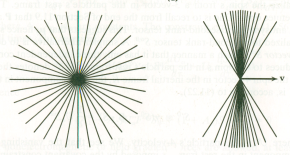
\includegraphics[width=.65\textwidth]{boost.png}
      \end{center}
      \caption{ \label{fig:boost} The electromagnetic field boosted and at rest. }
    \end{figure}
    The frequency modes of the electrostatic field are treated as photons. 
    The Weizs\"{a}cker-Williams approximation makes the calculation of 
      electromagnetic interactions with the nucleus tractable. 

    The Weizs\"{a}cker-Williams approximation begins with the equation for the 
      electric field of the projectile nucleus at rest. 
    To calculate the photon flux on the target nucleus, \DIFaddbegin \DIFadd{the }\DIFaddend electromagnetic field 
      only needs to be considered at the position of the target nucleus. 
    From the projectile's point of view, the target is moving and contributes
     $-vt$ to Eq.~\ref{eq:staticEFromTargtmp}, the equation for the electric 
     field of the projectile nucleus at rest.
    \begin{equation} \label{eq:staticEFromTargtmp}
        x'=-vt'\textrm{,}\qquad
        y'=b\textrm{,}\qquad
        z'=0\textrm{,}\qquad
        \vec{\mathbf{E'}}=\left(\frac{eZ}
         {4 \pi \epsilon_{0}\left(\left(-vt'\right)^{2}+b^{2}\right)^{3/2}}\right)
         \left(-vt'{\mathbf{\hat{x'}}+b\mathbf{\hat{y'}}}\right)\textrm{,}
    \end{equation}        
      where $b$ is the impact parameter
      defined as the distance of separation at closest approach, $v$ is the velocity of the 
      projectile nucleus, $Z$ is the number of protons in the nucleus, and $e$ 
      is the charge of the electron.
    Two simplifications occur due to the choice of coordinates in 
      Eq.~\ref{eq:staticEFromTargtmp}.
    The magnetic field is equal to zero, as the projectile is at rest, and
      the $z$ coordinate can be ignored, reducing the equation to two dimensions. 

    The Lorentz transformation converts the field equations in the 
      projectile's frame to equations in the target's frame.
    Eq.~\ref{eq:staticEFromTarg2tmp} gives the result of the transformation 
      from the projectile's primed frame to the target's rest frame for 
      the field components \cite{WWJackson}:
    \begin{eqnarray} \label{eq:staticEFromTarg2tmp}
        E_{x}'=E_{x}\textrm{,}\qquad
        \gamma\left(E_{y}'/c+\beta B_{z}'\right)=E_{y}/c\textrm{,}\qquad
        \gamma\left(E_{z}'/c=\beta B_{y}'\right)=E_{z}/c\textrm{,} \nonumber \\
        B_{x}'=B_{x}\textrm{,}\qquad
        \gamma\left(B_{y}'-\beta E_{z}'/c\right)=B_{y}\textrm{, and}\qquad
        \gamma\left(B_{z}'+\beta E_{y}'/c\right)=B_{z}\textrm{.}
    \end{eqnarray}
    The transformation equations for the fields, 
      Eq.~\ref{eq:staticEFromTarg2tmp}, and the transformation of the 
      coordinates reduce to Eq.~\ref{eq:staticEFromTarg3tmp} \cite{WWJackson}:
    \begin{eqnarray} \label{eq:staticEFromTarg3tmp}
        E_{x}'=E_{x}\textrm{,}\qquad
        \gamma E_{y}'=E_{y}\textrm{,}\qquad
        \gamma \beta E_{y}'/c=B_{z}\textrm{,}\nonumber \\
        ct'=\gamma ct\textrm{, and}\qquad
        x'=-\gamma \beta c t\textrm{.}
    \end{eqnarray}
    The Lorentz transformation reduces the six components of the 
      electromagnetic field in the target's frame to the three equations in 
      Eq.~\ref{eq:staticEFromTarg2tmp} by relating them to the fields \DIFdelbegin \DIFdel{of }\DIFdelend \DIFaddbegin \DIFadd{in }\DIFaddend the 
      projectile's frame. 

    By combining Eq.~\ref{eq:staticEFromTargtmp} and 
      Eq.~\ref{eq:staticEFromTarg2tmp}, equations for the electric and 
      magnetic fields in the target's rest frame are obtained 
        \begin{eqnarray} \label{eq:ebPframe} 
          \vec{\mathbf{E}}=\left( \frac{\gamma e Z}
           { 4 \pi \epsilon_{0} \left( \left( \gamma v t \right)^{2} 
           + b^{2}\right)^{3/2} }\right)
           \left(vt\mathbf{\hat{x}}+b\mathbf{\hat{y}}\right)\nonumber\textrm{, and} \\
           \vec{\mathbf{B}}=\frac{\gamma\beta e Z b}
           { 4 \pi c \epsilon_{0} \left( \left( \gamma v t \right)^{2} 
           + b^{2}\right)^{3/2} }
           \mathbf{\hat{z}}=
           \frac{\gamma\mu_{0}veZb}{4\pi\left(\left(\gamma v t \right)^{2}
           +b^{2}\right)^{3/2}}\mathbf{\hat{z}}.
        \end{eqnarray}
    If the impact parameter $b$ goes to zero, the target sits in the line of 
      the projectile particle's motion, and the denominator carries a factor of
      $\gamma$ squared. 
    When $vt$ goes to zero, the projectile particle position lays on the 
      $y$-axis, and the numerator carries a factor of $\gamma$. 
    This results in fields that are a factor of $\gamma^3$ higher in the 
      $y$ direction than in the $x$ direction (see Fig.~\ref{fig:boost}).  
    The boost compresses the electric field of the charge 
      in the direction of the boost and produces a magnetic field 
      resulting in a form similar to radiation.
    The point charge at ultra relativistic velocities produces a strong 
      electric field in the plane transverse to its motion resembling a plane 
      wave.

    Separating the electromagnetic field into even and odd functions of time 
      \DIFdelbegin \DIFdel{simplify }\DIFdelend \DIFaddbegin \DIFadd{simplifies }\DIFaddend the decomposition of the field equations into Fourier frequency 
      modes.
    The even functions decompose into cosine functions, odd functions 
      into sine functions. 
    The $y$-component of the electric field and the $z$-component of 
      the magnetic field are even functions in time, and the 
      $x$-component of the electric field is an odd function in time.
    Eq.~\ref{eq:fourier1tmp} gives the Fourier transformation integrals. 
    \begin{eqnarray} \label{eq:fourier1tmp}
        E_{x}(\omega)=\sqrt{\frac{2}{\pi}}\frac{eZ}{4\pi\epsilon_{0}b^{2}}
         \int^{\infty}_{0}\frac{\left(\gamma vt/b\right)\sin
         \left(\omega t\right)}
         {\left(\left(\gamma vt/b\right)^{2}+1\right)^{3/2}}dt\textrm{,} \nonumber\\
          E_{y}(\omega)=\sqrt{\frac{2}{\pi}}\frac{\gamma eZ}
         {4\pi\epsilon_{0}b^{2}} \int^{\infty}_{0}\frac{\cos(\omega t)}
         {\left(\left(\gamma vt/b\right)^{2}+1\right)^{3/2}}dt\textrm{,  and}\\
          B_{z}(\omega)=\frac{\beta E_{y}(\omega)}{c}.\nonumber
    \end{eqnarray}
    The solutions to the integrals of Eq.~\ref{eq:fourier1tmp} are the following
      \cite{WWFermi}:
    \begin{eqnarray}  \label{eq:fourier2tmp}
      u=\frac{\gamma v t}{b}\textrm{,}\qquad du\left(\frac{b}{\gamma v}\right)=dt\textrm{,}\qquad
      \omega'=\frac{\omega b}{\gamma v}\textrm{,}\nonumber \\
      \int^{\infty}_{0}\frac{u \sin(\omega'u)}{\left(u^{2}+1\right)^{3/2}}du
      =\omega'K_{0}(\omega')\textrm{, and}\qquad
      \int^{\infty}_{0}\frac{\cos(\omega'u)}{\left(u^{2}+1\right)^{3/2}}
      =\omega'K_{1}(\omega').
    \end{eqnarray}
    In Eq.~\ref{eq:fourier2tmp}, $\omega$ can be related to the energy of a 
      photon by $E=\hbar\omega$.
    The components of the electric field in terms of $\omega$ are:
    \begin{equation} \label{eq:fourier3tmp}
        E_{x}(\omega)=\sqrt{\frac{2}{\pi}}\frac{eZ}{4\pi\epsilon_{0}b^{2}}
     \frac{b}{\gamma v}\frac{\omega b}{\gamma v}K_{0}
     \left(\frac{\omega b}{\gamma v}\right)\textrm{, and}\qquad
      E_{y}(\omega)=\sqrt{\frac{2}{\pi}}\frac{\gamma eZ}{4\pi\epsilon_{0}b^{2}}
     \frac{b}{\gamma v}\frac{\omega b}{\gamma v}K_{1}
     \left(\frac{\omega b}{\gamma v}\right).\qquad
    \end{equation}
    The $y$-component of the electric field does not have a factor of $t$ in 
      the numerator \DIFaddbegin \DIFadd{in Eq.~\ref{eq:fourier1tmp}}\DIFaddend , therefore the factor of $\gamma$ 
      remains outside of the integral \DIFdelbegin \DIFdel{.
    }\DIFdelend \DIFaddbegin \DIFadd{for the Bessel functions in 
      Eq.~\ref{eq:fourier3tmp}.
    }\DIFaddend In Eq.~\ref{eq:fourier3tmp}, $E_{y}$ carries an additional factor of 
      $\gamma$ in the numerator relative to the $E_{x}$, therefore in the case
      when $\gamma >> 1$, $E_{x}$ can be neglected. 

    When $v$ approaches $c$, $\beta \approx 1$, the $y$-component of the 
      electric field and the $z$-component of the magnetic field are related by 
      a factor of $c$, $E_{y}/c=B_{z}$.
    $E_{y}$ is approximately equally to $\gamma$ $E_{x}$ because $K_{0}(x)$ is 
      smaller than $K_{1}(x)$ for all $x$. 
    The conditions imposed by the ultra-relativistic limit result in the 
      following relationship
    \begin{equation} \label{eq:ultraRelAprox}
      \gamma \gg 1 \Rightarrow \gamma E_{x} \gg E_{x} \Rightarrow E_{y} \gg E_{x} \textrm{.}
    \end{equation}
    The six field components \DIFaddbegin \DIFadd{are }\DIFaddend reduced to one electric component and one 
      perpendicular magnetic field component, which have a configuration 
      identical to a plane wave. 

    As with plane waves, the energy per area per time transferred by 
      the electromagnetic field is given by the Poynting vector.
    The Poynting vector takes the simple form of a plane pulse propagating in 
     the $x$ direction as given by
    \begin{equation} \label{eq:poyntingVectortmp}
        \vec{\mathbf{S}}\equiv
        \vec{\mathbf{E}}\times\vec{\mathbf{B}}/\mu_{0}=
        \left(E_{y}^{2}/c\mu_{0}\right)\mathbf{\hat{x}}=
        c\epsilon_{0}E_{y}^{2}\mathbf{\hat{x}}.
    \end{equation}
    The Poynting vector relates to the fluence (energy per unit area) 
      by the expression \cite{WWBrau} 
    \begin{equation} \label{eq:fluencytmp}
        I(b)=\mathbf{\hat{x}}\cdot\int^{\infty}_{0}\vec{\mathbf{S}}d\omega=
         \int^{\infty}_{0}\left(c\epsilon_{0}E_{y}^{2}\right)d\omega=
         \int^{\infty}_{0}\left(\frac{dI}{d\omega}\right)d\omega,
    \end{equation}
      and the spectral fluence (energy per area per frequency) is given 
      by
    \begin{equation} \label{eq:specturalFluencytmp}
      \frac{dI}{d\omega}=c\epsilon_{0}E_{y}^{2}=
       \frac{e^{2}Z^{2}c}{4\pi^{3}b^{2}v^{2}\epsilon_{0}}
       \left(\frac{\omega b}{\gamma v}\right)^{2}
         K_{1}^{2}\left(\frac{\omega b}{\gamma v}\right)=
        \alpha\hbar\left(\frac{Z}{b\beta\pi}\right)^{2}
         \left(\frac{\omega b}{\gamma v}\right)^{2}
       K_{1}^{2}\left(\frac{\omega b}{\gamma v}\right).
    \end{equation}
    The spectral fluence given by Eq.~\ref{eq:specturalFluencytmp} 
      relates the frequency to energy. 
    The quantum mechanical equation, $E=\hbar\omega$, gives the energy of a 
      photon, which is related to the spectral fluence. 
    The relationship between the photon number density and the spectral fluence
      is \cite{WWJackson}
    \begin{equation}  \label{eq:photonFluxtmp}
        \frac{dI}{d\omega}d\omega=\hbar\omega N(\omega)d(\hbar\omega)
        \Rightarrow \frac{1}{\hbar^{2}\omega}\frac{dI}{d\omega}=N(\omega).
    \end{equation}
    Substituting Eq.~\ref{eq:specturalFluencytmp} into 
      Eq.~\ref{eq:photonFluxtmp} yields the semiclassical photon flux:
    \begin{equation} \label{eq:photonFluxFinaltmp}
      N(\omega,b)=\frac{\alpha}{\hbar\omega}
       \left(\frac{Z}{b\beta\pi}\right)^{2}
       \left(\frac{\omega b}{\gamma v}\right)^{2}
       K_{1}^{2}\left(\frac{\omega b}{\gamma v}\right).
    \end{equation}
    This replaces the classical electric field of a point charge with a 
      semiclassical field of photons. 
    The photon flux in Eq.~\ref{eq:photonFluxFinaltmp} provides the 
      electromagnetic input to the \JPsi{} photoproduction cross section 
      calculation. 

  \section{\label{sec:vdmTheory}The STARlight model}
    The STARlight model for calculating the \JPsi{}
      photoproduction cross section has three main components.
    The STARlight approach is constructed from the Weizs\"{a}cker-Williams 
      photon flux, uses the vector meson dominance fit to the proton-electron data, 
      and uses the Glauber model for calculating the nuclear cross sections from 
      the proton-electron cross sections.
    The Weizs\"{a}cker-Williams photon flux provides the probe. 
    The proton-electron scattering data combine with the Glauber model  
      create a picture of the initial state of the nucleus. 
    Each of the different approaches discussed in this thesis to calculating 
      the UPC \JPsi{}  photoproduction cross section use these same elements.
    However, the different models each use the last two elements differently 
      to produce different pictures of the nucleus and different cross 
      sections values. 

    The photon flux in the photoproduction cross section calculation must be 
      finite in order for the cross section to be meaningful.
    The Weizs\"{a}cker-Williams approximation, Eq.~\ref{eq:photonFluxFinaltmp}, 
      diverges at $b=0$.
    The probability of the nuclei interacting would exceed one if the photon 
      flux were infinite. 
    Special treatment of impact parameter, $b$, where the colliding nuclei 
      overlap eliminates the divergency. 

    A convolution of the photon flux with the nucleon number density functions 
      removes the divergency at $b=0$. 
    The nucleon density of a single nucleus is given by
    \begin{equation} 
      \rho_{A}(s)=\frac{\rho_{0}}{1+exp[(s-R_{WS})/d)]}\textrm{,}
      \label{eq:woodsSaxon}
    \end{equation}
    where $s$ is the distance from the center of the 
      nucleus, $R_{WS}$ is the radius of the nucleus, and $d$ is the skin depth, 
      which determines how quickly the nucleon density falls off beyond the 
      nuclear radius. 
    In Eq.~\ref{eq:TaNuc} the depth of the nucleus is integrated out leaving
      just the transverse dimension in $T_{A}$.
    The average number of nucleons in the overlap region is given by a
      convolution of $T_A$ from each of the two nuclei to produce 
    \DIFaddbegin \DIFadd{The average number of nucleons in the overlap region is given by a 
      convolution of $T_A$ from each of the two nuclei to produce nuclear overlap 
      integral, }\DIFaddend $T_{AA}$\DIFaddbegin \DIFadd{,
    }\DIFaddend \begin{eqnarray} \label{eq:TaNuc}
      T_{A}(\vec{r})=\int{dz\rho_{A}(\sqrt{|\vec{r}|^{2}+z^{2}})}\textrm{, and} \nonumber \\ 
      T_{AA}(|\vec{b}|)=\int{d^{2}\vec{r}T_{A}(\vec{r})T_{A}(\vec{r}-\vec{b})}\DIFaddbegin \textrm{\DIFadd{.}}
    \DIFaddend \end{eqnarray}
    \DIFaddbegin \DIFadd{For a given impact parameter $b$, the product of $T_{AA}(|\vec{b}|)$ and
      $\sigma_{NN}$ gives the average number of nucleon-nucleon collisions. 
    }\DIFaddend It is $T_{AA}$ that modulates the photon flux. 
    As input to the Poisson distribution, $T_{AA}$ reduces 
      Eq.~\ref{eq:photonFluxFinaltmp} at values of $b$ where the nuclei overlap 
      significantly and eliminates the divergency in the photon flux. 
    \DIFdelbegin %DIFDELCMD < 

%DIFDELCMD <     %%%
\DIFdelend The convolution of the photon flux with the $b$-dependent probability that 
      no nucleon-nucleon collisions occur removes the divergency in 
      Eq.~\ref{eq:photonFluxFinaltmp}. 

    The Poisson distribution gives the probability that no collisions 
      occur at a given $b$ using the mean number of nucleons in the overlap 
      region given by $T_{AA}$:
    \begin{equation} \label{eg:poisNoCol}
      P_{0}(b)=exp[-T_{AA}(b)\sigma_{NN}],
    \end{equation}
    where $\sigma_{NN}$ is the cross section for a 
      nucleon-nucleon interaction, which gives the probability that a collision
      will occur given the average number of nucleons in the overlap region.
    The \DIFdelbegin \DIFdel{average photon flux }\DIFdelend \DIFaddbegin \DIFadd{photon flux is averaged }\DIFaddend over impact parameter \DIFdelbegin \DIFdel{can be calculated 
      from the }\DIFdelend \DIFaddbegin \DIFadd{by }\DIFaddend integration of the 
      $b$-dependent photon flux with the $b$-dependent probability of having no 
      nucleon-nucleon interactions: 
    \begin{equation} \label{eq:fluxMod}
      \frac{dN_{\gamma}(k)}{dk}=\int_{0}^{\infty}{2\pi bdbP_{0}(b)
         \int_{0}^{R}{\frac{rdr}{\pi R^{2}_{A}}\int_{0}^{2\pi}d\phi
         \frac{d^{3}N_{\gamma}(k,b+r\cos(\phi))}{dkd^{2}r}}}.
    \end{equation}
    Although Eq.~\ref{eq:fluxMod} goes down to $b=0$ where the photon flux is 
      infinite, the fact that the probability of having a nucleon-nucleon collisions 
      is high eliminates the divergency.

    A power-law fit to the proton photoproduction data gives an analytic 
      expression for the energy dependence of the proton photoproduction 
      cross section.
    The fitting function depends on the photon-proton center of mass energy. 
    The parameterization of the forward proton photoproduction cross section 
      fit:
    \begin{equation} \label{eq:proElFit}
      \frac{d\sigma(\gamma p\rightarrow Vp)}{dt}\Big|_{t=0}
        =b_{v}(XW^{\epsilon}+YW^{-\eta}),
    \end{equation}
    where $W$ is the center of mass energy of the proton-photon system in 
      Eq.~\ref{eq:proElFit}.
    The remaining variables in Eq.~\ref{eq:proElFit} are power-law fit 
      parameters.  
    The $XW^{\epsilon}$ term characterizes pomeron mediated interactions, and
      the $YW^{\eta}$ term characterizes meson mediated interactions~\cite{vmd1999}. 
    \JPsi{}'s high mass relative to the $\pi$ and $\rho^{0}$ renders the second 
      term in Eq. ~\ref{eq:proElFit} negligible as the term falls rapidly with
      increasing $W$. 
    Eq.~\ref{eq:proElFit} allows for extrapolation and interpolation of the 
      measured forward proton photoproduction cross section. 
    The fit to the data provides estimates for energies that have not yet been 
      probed experimentally.
    The proton photoproduction cross sections from the electron-proton 
      scattering data is a direct input to the STARlight model. 
    In this method, a power-law fit to the proton photoproduction data is the 
      input for the Glauber calculation. 

    Vector meson dominance and the optical theorem allow for the calculation of 
      the total proton-meson scattering cross section from the fit given by 
      Eq.~\ref{eq:proElFit}. 
    The optical theorem relates the total cross section, $\sigma$, 
      to the corresponding forward scattering cross section, 
      $d\sigma/dt|_{t=0}$, where $t$ is the momentum transfer squared.
    The most likely fluctuations of the photon are to vector mesons because of 
      the quantum numbers of the photon.
    \DIFaddbegin \DIFadd{Due to this consideration, vector meson dominance asserts that the only the 
      vector meson fluctuates of the photon need to be considered. 
    }\DIFaddend The forward scattering cross section is given by the following
    \begin{eqnarray} \label{eq:STARlightforwardScat}
      \frac{d\sigma(\gamma p\rightarrow Vp)}{dt}\Big|_{t=0}=
      \frac{4\pi \alpha}{f^{2}_{v}(M_{V},\Gamma_{l^{+}l^{-}})}\frac{d\sigma(Vp\rightarrow Vp)}{dt}
        \Big|_{t=0} \textrm{,} \nonumber \\
      \sigma(Vp)_{tot}^{2}=16\pi\frac{d\sigma(Vp\rightarrow Vp)}{dt}\Big|_{t=0} \textrm{,}
    \end{eqnarray}
      where $M_{V}$, is the mass of the vector meson, and $\Gamma_{l^{+}l^{-}}$, 
      is leptonic decay width. 
    The result of combining vector meson dominance and the optical theorem 
      in Eq.\ref{eq:STARlightforwardScat} provides the cross section for a meson to 
      scatter off a proton.

    The Glauber model allows for Eq.~\ref{eq:STARlightforwardScat}, the proton-meson
      scattering cross section, to be used to calculate a nucleus-meson 
      scattering cross section. 
    The Glauber model is used to calculate nuclear cross sections from 
      nucleon interaction cross sections by use of $T_{AA}$. 
    The combination of the mean number of nucleons in the overlapping region
      of a nucleus-nucleus collision, $T_{AA}$, the nucleon cross section, 
      $\sigma$, and the Poisson distribution make-up the core of the Glauber 
      model. 
    For the total nucleus-meson scattering cross section, the equation has the 
      following form:
    \begin{equation} \label{eq:glauber}
      \sigma_{tot}(VA)=\int d^{2}\vec{r}(1-e^{-\sigma_{tot}(Vp)T_{AA}(\vec{r})}).
    \end{equation}
    In Eq.~\ref{eq:glauber}, the term $e^{\sigma_{tot}(Vp)T_{AA}}$ gives the
      probability of having no meson-nucleon scatterings from the Poisson 
      distribution. 
    The probability of having at least one scattering is given by subtracting 
      one from the term  $e^{\sigma_{tot}(Vp)T_{AA}}$ in Eq.~\ref{eq:glauber}.

    Reversing the process used for the proton, Eq.~\ref{eq:glauber}, the meson 
      nucleus scattering cross section, relates to forward nuclear 
      photoproduction cross section through the optical theorem. 
    Using the optical theorem, the nuclear photoproduction cross section is 
      given by 
    \begin{eqnarray} \label{eq:optTheA}
      \frac{d\sigma(\gamma A\rightarrow VA)}{dt}\Big|_{t=0}=
      \frac{\alpha\sigma_{tot}^{2}(VA)}{4\pi f_{v}^{2}}\nonumber \textrm{,}\\
      \sigma(\gamma A\rightarrow VA)=\frac{d\sigma(\gamma A\rightarrow VA)}{dt}
      \Big|_{t=0}\int_{t_{min}}^{\infty}dt|F(t)|^{2} \textrm{,}
    \end{eqnarray}
    where $F$ is the Fourier transform of the nuclear density function, 
      $\rho_{A}$.
    Eq.~\ref{eq:optTheA} is joined with the photon flux incident on the nucleus 
      resulting in the following
    \begin{equation} \label{eq:finalSTARlightResult}
      \sigma(AA\rightarrow AAV)=2\int{dk\frac{dN_{\gamma}}{dk}
                    \sigma(\gamma A\rightarrow VA)}.
    \end{equation}
    The factor of 2 in Eq.~\ref{eq:finalSTARlightResult} comes from the fact that 
      both of the two colliding nuclei contribute. 
    Vector meson production rates in UPC collisions can be calculated
      by Eq.~\ref{eq:finalSTARlightResult}.
    In this thesis the measured UPC \JPsi{} cross section is compared to the
      STARlight predictions. 

  \section{The Adeluyi and Bertulani model \label{sec:pQCDapp}}
    To calculate the UPC \JPsi{} photoproduction cross section, the Adeluyi 
      and Bertulani model uses the nuclear gluon density to characterize the 
      nucleus and the Weizs\"{a}cker-Williams approximation for the probing 
      photon flux. 
    The AB method combines these components such that the nuclear gluon 
      density is a direct variable.
    The nuclear gluon density term in the AB formulation allows for 
      the use of a variety of nuclear gluon density models.
    A range of nuclear gluon densities are present in the available models
      resulting in a wide range of possible cross section values. 
    The UPC \JPsi{} photoproduction cross section is correlated with the gluon
      density of the nucleus, increasing with higher densities and decreasing 
      with lower densities. 
    In the AB approach, the calculation of the UPC \JPsi{} photoproduction 
      cross section allows experiments to constrain many different nuclear 
      gluon density models. 

    In the AB method, the photon interacts with the nucleus by fluctuating to 
      a quark-anitquark pair.
    For \JPsi{}, the photon fluctuates to a $c\bar{c}$ pair. 
    The probability for the photon to fluctuate to a $c\bar{c}$ pair
      depends on the $M_{J/\psi}$, the mass of \JPsi{}, $\Gamma_{l^{+}l^{-}}$, 
      the \JPsi{} leptonic decay width, and $\alpha$, the electromagnetic 
      coupling constant.
    These three variables connect the $c$ quark to the electromagnetic force 
      mediator, the photon. 
    Recast as a $c\bar{c}$ pair, the photon couples to the nuclear gluon 
      density.
    The AB method uses the fluctuation of the photon to a $c\bar{c}$ 
      pair as the foundation for calculating the forward \JPsi{} 
      photoproduction cross section. 

    The $c\bar{c}$ pair arising from the photon fluctuation scatters off the 
      gluons of the nucleus. 
    The density of gluons in the nucleus determines how likely and therefore 
      how large the cross section is for the quarks to scatter and form a 
      \JPsi{}.
    The forward scattering cross section is the portion of those scattering 
      events which transfer the minimum amount of momentum between the 
      photon and the nucleus. 
    The forward cross section for \JPsi{} photoproduction in the nucleus has 
      the following form \cite{pQCD2011.08}:
    \begin{equation} \label{eq:ABfowardScat}
      \frac{d\sigma_{\gamma A\rightarrow J/\psi A}}{dt}\Big|_{t=0}=\xi_{J/\psi}
        \Big(\frac{16\pi^{3}\alpha_{s}^{2}\Gamma_{l^{+}l^{-}}}{3\alpha 
        M_{J/\psi}^{5}}\Big)[xG_{A}(x,\mu^{2})]^{2},
    \end{equation}
      where $\xi_{J/\psi}$ is an experimentally derived 
      correction factor, $\alpha_{s}$ is the strong coupling constant, $x$ is 
      the momentum faction of the nucleus the scattering gluons carry, and 
      $G_{A}$ is the gluon density of the nucleus. 
    Both the $c$ and $\bar{c}$ couple to the gluon density, and the double 
      coupling results in the squared dependence of the cross section on the 
      gluon density in Eq.~\ref{eq:ABfowardScat}. 
    Fitting Eq.~\ref{eq:ABfowardScat} to proton-electron scattering data 
      sets $\xi_{J/\psi}$ \cite{pQCD2011.08}.
    The forward scattering cross section given by Eq.~\ref{eq:ABfowardScat} 
      connects the photon flux to the gluon density and provides the input to 
      calculate the total cross section by the optical theorem. 

    The optical theorem relates the forward cross section in 
      Eq.~\ref{eq:ABfowardScat} to the total photoproduction cross section. 
    The total cross section gives the probability that a photon incident on 
      the nucleus will produce a \JPsi{} regardless of the momentum transfered 
      in the interaction. 
    The total cross section equation is given by
    \begin{equation} \label{eq:ABtotXSec}
      \sigma_{\gamma A\rightarrow J/\psi A}(k)=
      \frac{d\sigma_{\gamma A\rightarrow J/\psi A}}{dt}\Big|_{t=0}
      \int_{t_{min}(k)}^{\infty}dt|F(t)|^{2},
    \end{equation} 
      where $t_{min}=(M_{J/\psi}^{2}/4k\gamma_{L})^2$, which is the minimum 
      amount of momentum transfer required to produce a \JPsi{} 
      given the photon wave number $k$.
    The $k$ dependence of $t_{min}$ translates to the rapidity 
      dependence of the total cross section.
    The total cross section for photoproduction, Eq.~\ref{eq:ABtotXSec}, 
      provides the input to Eq.~\ref{eq:ltaRapDist}, 
      which gives the rapidity dependence of the UPC photoproduction cross 
      section. 
    Eq.~\ref{eq:ABtotXSec} as input to Eq.~\ref{eq:ltaRapDist} allows for 
      experimental comparison of the AB method to measurements of UPC 
      photoproduction cross sections. 
    With the AB method's direct use of the nuclear gluon density in 
      Eq.~\ref{eq:ABfowardScat}, the AB method allows for experimental 
      exploration of any gluon density model. 

  \section{\label{sec:ltaTheory}Leading Twist Approach Derivation}
    The Leading Twist Approach is another method for calculating UPC 
      photoproduction cross sections. 
    Contrary to the STARlight model, the LTA model introduces additional 
      nuclear effects originating from modification of the nuclear gluon
      density. 
    The LTA method uses the Weizs\"{a}cker-Williams approximation to calculate 
      the photon flux created by the colliding nuclei. 
    As in the STARlight method, the probability of having no hadronic collisions 
      modulates the flux.
    The photon flux for the LTA method has the following form \cite{lta2011.09}:
    \begin{equation} \label{eq:ltaPhotonFlux}
      n_{\gamma/A}^{i}(\omega_{\gamma})=\frac{2\alpha Z^{2}}{\pi}\int_{b_{min}}^{\infty}
        db\frac{x^{2}}{b}\Big[K_{1}^{2}(x)+\frac{K_{0}^{2}(x)}{\gamma_{L}^{2}}\Big]
        P_{0}(b)P_{C}^{i}(b)\textrm{,} 
    \end{equation}
    where $x=\frac{\omega b}{\gamma_{L}}$, and $K_{0}^{2}(x)$ term contributes 
      a photon flux in the transverse direction, and $P_{C}^{i}(b)$ is an 
      modulation factor that requires various additional interactions. 
    These interactions result in emission of neutrons from the 
      receding nuclei as the nuclei relax from excited states. 
    The terms $P_{C}^{i}$ and $K_{0}$ provide additional ways to distinguish UPC
      events from nuclear collisions experimentally but leave the underlying 
      interaction mechanism the same. 
    For example, the additional terms in the LTA formulation of the photon flux
      produce calculations of asymmetric neutron emission, which separate UPC 
      events from nuclear collisions.  

    The LTA model derives the nucleon cross section from derivations
     of the nucleon gluon densities from electron-proton scattering data and
     leading order perturbative quantum field theory calculations.
    The forward photoproduction cross section of the nucleon has the following
     form \cite{lta2011.09}:
   \begin{equation} \label{eq:ltaFowardPhotoXSec}
     \frac{d\sigma_{\gamma N\rightarrow J/\psi N}(t=0)}{dt}=\frac{16\Gamma_{l^{+}l^{-}}\pi^{3}}
     {3\alpha M_{J/\psi}^{5}}[\alpha_{s}\mu^{2}xG_{N}(x,\mu^{2})]^{2}\textrm{,}
   \end{equation}
     where $G_{N}$ is the gluon density of the nucleon, $x$ is the fraction of
     the nucleon's momentum the gluon carries, and $\mu$ is related
     to momentum at which the nucleon is being probed, which is equal to 
     $M_{J/\psi}/2$ for \JPsi{} photoproduction.
   By connecting the gluon density to the cross section, Eq.~\ref{eq:ltaFowardPhotoXSec}
     allows for the gluon density to be experimentally probed. 

   The LTA model exploits the optical theorem to relate the forward 
     photoproduction cross section of the nucleon to the nuclear cross section. 
   The relation is
   \begin{equation} \label{eq:ltaOptTheWNucMo}
     \sigma_{\gamma A\rightarrow J/\psi A}(\omega)=
     \frac{d\sigma_{\gamma N\rightarrow J/\psi N}}{dt}(\omega,t_{min})
     R_{g}^{2}\int_{t_{min}}^{\infty}dt|F(t)|^{2}\textrm{,}
   \end{equation}
   where $R_{g}$ is the nuclear modification function, the ratio between the gluon 
     density of the nucleon, $G_{N}$, to the gluon density of the nucleus, 
     $G_{A}$.
   As with the STARlight method, the optical theorem relates the forward cross 
     section, $\frac{d\sigma_{\gamma N\rightarrow J/\psi N}}{dt}(\omega,t_{min})$,
     to the total cross section, $\sigma_{\gamma A\rightarrow J/\psi A}$. 

   From Eq.~\ref{eq:ltaOptTheWNucMo}, the LTA method can predict the angular 
     distribution of photoproduced \JPsi{} with respect to the beam axis. 
   The angular distribution is expressed in the form of the rapidity 
    dependency of the UPC photoproduction cross section given by 
   \begin{equation} \label{eq:ltaRapDist}
     \frac{d\sigma_{A_{1}A_{2}\rightarrow A_{1}A_{2}J/\psi}}{dy}=
       n_{\gamma/A_{1}}(y)\sigma_{\gamma A_{2}\rightarrow J/\psi A_{2}}(y)
       +n_{\gamma/A_{2}}(-y)\sigma_{\gamma A_{1}\rightarrow J/\psi A_{1}}(-y)\textrm{,} 
   \end{equation}
   where $y=ln\left(\frac{2\omega}{M_{J/\psi}}\right)$.
   Eq.~\ref{eq:ltaRapDist} is comprised of two terms, one for photons from the
     forward going nucleus interacting with the backward going nucleus, and 
     a second for the reverse situation. 
   The integration of Eq.~\ref{eq:ltaRapDist} over $y$ produces the factor of 2 
     that is present in Eq.~\ref{eq:finalSTARlightResult}.
   The rapidity distribution of the photoproduction cross section given in 
   Eq.~\ref{eq:ltaRapDist} provides a more detailed prediction and allows for
     more direct experimental \DIFdelbegin \DIFdel{comparison}\DIFdelend \DIFaddbegin \DIFadd{comparisons}\DIFaddend .

  \section{\label{sec:nucBreakUp}Photon-induced nuclear break-up}
    In addition to the photoproduction of quark anti-quark resonances such as 
      the \JPsi{}, photo-nuclear interactions can also result in emission of a 
      neutron from the struck target nucleus.
    To calculate the cross section for neutron emission in UPC events, the 
      photon flux calculated from the Weizs\"{a}cker-Williams approximation is
      combined with the nuclear photon absorption cross section. 
    The absorption of photons can be described by two processes, namely the 
      Giant Dipole Resonance (GDR), and the dissociation of deuterium.
    In this section, the theoretical description of photon-induced nuclear 
      break-up is discussed.

    Following the formulation in~\cite{emPCite4}, the cross section for a
      nucleus to absorb a photon, $\sigma_{PN}$, is given by 
      \begin{equation}
        \sigma_{PN}=\sigma_{GDR}+\sigma_{QD}.
        \label{eq:photoNucDis}
      \end{equation}
    The Giant Dipole Resonance (GDR) cross section, $\sigma_{GDR}$ is the result
      of the collective motion of the protons relative to the neutrons and 
      dominates at lower photon frequencies.
    The Quasi-Deuterium (QD) cross section, $\sigma_{QD}$, represents the 
      nucleus as a collection of proton-neutron pairs (deuterium) and dominates 
      at higher photon energies.

    There are two models for the GDR: the Goldhaber and Teller model, and the 
      Steinwedel and Jensen model.
    Goldhaber and Teller treats the protons and neutrons as two separate and 
      ridged density profiles that, when excited, oscillate with respect to 
      each other \cite{emPCite6}.
    Steinwedel and Jensen modeled the protons and neutrons as fluids contained 
      in a single sphere that have shifting density profiles \cite{emPCite6}.

    In the Goldhaber and Teller model, the potential that holds protons and 
      neutrons together depends on the difference of the neutron and proton 
      densities squared.
    Assuming the neutron and proton densities have the same shape, if the two 
      fully overlap, there is no difference in the densities and the
      potential energy is zero.
    If the two density distributions are separated, the overlap in the shape 
      will not cancel.
    In the separated configuration, there will be a non-zero potential energy.
    The potential energy has the form of a harmonic oscillator with a spring 
      constant that depends on the initial density distribution \cite{emPCite6}
      given by 
    \begin{equation}
      U=\frac{1}{2}Kz^{2}, \qquad K=k\int d^{3}r\left(\nabla\rho_{0}\right)^{2}.
      \label{eq:potEnGDR}
    \end{equation}
    If the nucleus has a shape cut off in density at its edge, then the 
      integral is dominated  by the region at the surface, and the spring 
      constant, $K$, becomes proportional to $A^{2/3}$, where $A$ is the mass
      number of the nucleus.
    The surface area of a sphere is proportional to its volume to the $\textrm{2/3}$
      power explaining the mass dependence.
    Due to this dependence, the frequency of the giant dipole resonance in the 
      Goldhaber and Teller model is given by
    \begin{equation}
      \omega=\sqrt{\frac{K}{M}} \propto \sqrt{\frac{A^{2/3}}{A}}=A^{-1/6}.
      \label{eq:omegaGDR}
    \end{equation}
    This dependence describes light nuclei well, but it does not describe 
      heavier nuclei \cite{emPCite6}.
    The Steinwedel and Jensen model can be used to describe heavier nuclei.
    In this model, the proton and neutron fluids are 
      confined to a single sphere where they are allowed to slosh back and 
      forth creating the same effect as the Goldhaber and Teller model.
    Here there is no global separation of the proton and neutron fluids.
    The dipole is created by under-densities and over-densities of the proton and
      neutron fluids.
    It can be shown that this results in a frequency of oscillation which 
      depends on one over the radius of the nucleus \cite{emPCite6}:
    \begin{equation}
      \omega \propto \frac{1}{R} \propto A^{-1/3}.
      \label{eq:omegaGDRSJ}
    \end{equation}
    As before, the relationship in Eq.~\ref{eq:omegaGDRSJ} arises from the geometry of a sphere.
    The dependence of the giant dipole resonance that is seen in the Steinwedel 
      and Jensen model describes medium and heavier mass nuclei well.
    Empirically, both models are put together to give the following mass 
      number dependence of the dipole resonance \cite{emPCite6}
    \begin{equation}
      E_{GDR}=32.2A^{-1/3}+20.6A^{1/6}.
      \label{eq:enGDR}
    \end{equation}

    In order to compute the effect of an excitation in either model, 
      the harmonic oscillator solutions found earlier can be driven by an 
      interacting force.
    The resulting differential equation can then be solved using a Fourier 
      transform to eliminate the time derivatives.
    In this model the driven harmonic has the following Lorentzian form:
    \begin{equation}
      \sigma_{GDR}(E_{\gamma})=\frac{\sigma_{max}E_{\gamma}\Gamma_{GDR}^{2}}
      {\left(E_{\gamma}^{2}-E_{GDR}^{2}\right)^{2}+E_{\gamma}^{2}\Gamma^{2}},
      \label{eq:gdrRes}
    \end{equation}
      where $\sigma_{max}$ is the maximum cross section reached when $E_{\gamma}$ = 
      $E_{GDR}$; $E_{GDR}$ is the peak resonance energy, and $\Gamma_{GDR}$ is 
      the width of the resonance.
    The width of this distribution lies in a range from 4-8 
      MeV and depends on the orbital arrangement to the neutrons and protons in
      the given nucleus \cite{emPCite6}.

    For higher energy photons, the quasi-deuterium cross section is needed.
    The nucleus is treated as a collection of proton-neutron pairs, which are 
      screened by the rest of the nucleus, in the quasi-deuterium approach.
    This behavior is modeled by \cite{emPCite4}
    \begin{equation}
      \sigma_{QD}(E_{\gamma})=L\frac{(L-A)Z}{A}\sigma_{d}(E_{\gamma})F(E_{\gamma}),
      \label{eq:qdSigma}
    \end{equation}
    where $\sigma_{d}$ is the deuterium disintegration cross section for 
      $\gamma+d$ $\rightarrow$ $p+n$;
    $F$ is a function from Pauli blocking of fermions, and $L$ is 
      an empirical parameter set by data to 6.5 \cite{emPCite4}.
    Certain energy levels are not available to the products of the deuterium 
      disintegration process because of the presence of the rest of the nucleus.
    The result is a reduction of the cross section relative to free deuterium.

    $F$ can be modeled with an exponential cutoff below 20 MeV, a polynomial in 
      the intermediate range with nearly linear dependence on $E_{\gamma}$, and 
      an inverted exponential above 140 MeV, pushing $F$ to one at higher 
      values of $E_{\gamma}$ \cite{emPCite4}.
    Essentially, the model at low photon energies disallows deuterium 
      disintegration because the products have no available state to occupy, 
      and at high energies the rest of the nucleus becomes transparent and 
      looks more and more like a collection of deuterium.
    The deuterium disintegration cross section is found empirically and is fit 
      to the following function \cite{emPCite4}:
    \begin{equation}
      \sigma_{d}(E_{\gamma})=61.2\left(E_{\gamma}-2.224\right)^{3/2}/E_{\gamma}.
      \label{eq:deDisSigma}
    \end{equation}
    In order to produce a final state for the target nucleus, a branching ratio
      is needed.
    The branching ratio gives the probability that the photo-excited nucleus 
      will end up in a particular state.
    This determines the sort of emission that will result from the 
      de-excitation process \cite{emPCite4}.

    All the tools are now assembled to calculate the cross section for neutron
      emission.
    The first step in the calculation is to assume that the number of photons 
      absorbed by either nucleus in the collision obeys the Poisson 
      distribution \cite{emPCite3,emPCite4}.
    The average number of absorptions as a function of impact parameter, $m(b)$,
      \begin{equation}
        m(b)=\int^{\omega_{max}}_{\omega_{min}}N(\omega,b)\sigma_{PN}(\omega)d\omega\textrm{.}
        \label{eq:meanOfSigma}
      \end{equation}
      where $\sigma_{PN}$ is the photo-nuclear cross section, and $N$ is the 
      photon flux (see Eq.~\ref{eq:photonFluxFinaltmp}).

   In \cite{emPCite4}, the probability of any final state $i$ due to the 
      absorption of a single photon is given by
    \begin{equation}
      P_{i}(b)=\int^{\omega_{max}}_{\omega_{min}}P_{a}(b,1)q(b,\omega)f_{i}(\omega)d\omega=
      e^{-m(b)}\int^{\omega_{max}}_{\omega_{min}}N(b,\omega)\sigma_{PN}(\omega)f_{i}(\omega)d\omega,
      \label{eq:photonProi}
    \end{equation}
    where $P_{a}$ is the probability that the target absorbs a single photon as 
      calculated by following the Poisson distribution; $q$ is the probability 
      that the photon will have the frequency $\omega$, and $f_{i}$ is the 
      branching ratio to a given final state.
    The following equation describes $q$ \cite{emPCite5}
    \begin{equation}
      q(b,\omega)=\frac{N(b,\omega)\sigma_{PN}(\omega)}{m(b)}
      \label{eq:freqProb}
    \end{equation}

    Integrating over the impact parameter to get an area that 
      is weighted by the probability functions gives \cite{emPCite3,emPCite4}
      \begin{equation}
        \sigma_{i}=2\pi\int^{\infty}_{b_{0}}bP_{i}(b)db.
        \label{eq:sigmaPi}
      \end{equation}
    Three parameters arise when calculating the cross section in Eq.~\ref{eq:sigmaPi}, the 
      minimum impact parameter $b_{0}$, the minimum emitted photon frequency 
      $\omega_{min}$, and the maximum emitted photon frequency $\omega_{max}$.
    A minimum impact parameter ensures that the Bessel 
      function in the photon flux in Eq.~\ref{eq:photonFluxFinaltmp} is not
      evaluated at zero.
    At zero, the modified Bessel function does not converge.
    Physically, a minimum impact parameter is selected in order to separate the
      domains between electromagnetic interactions and the strong interactions 
      that happen inside the nucleus.
    To serve this end, the minimum impact parameter is set to the radius of the
      nuclei \cite{emPCite3,emPCite4}.
    This excludes collisions where the nuclei overlap in the calculation, and 
      ensures that only electromagnetic interactions are involved.

  \section{Experimental Results}
  One of the first \DIFdelbegin \DIFdel{UPC }\DIFdelend results from RHIC was \DIFaddbegin \DIFadd{a UPC measurement, }\DIFaddend the measurement of the 
    neutron spectrum from photon-induced nuclear break-up \cite{upcNeuPHENIX}.
  Neutrons due to the nuclear photon absorption are emitted with momenta on the
    order of the giant dipole resonance, about 60 MeV.
  Momenta of 60 MeV compared to the 100 GeV beam energy at RHIC result in 
    neutron emission at very small angles, $\sim 2 \textrm{mrad}$, relative to 
    the beam.
  These neutrons are captured by calorimeters, which are set in line with the 
    beam called Zero Degree Calorimeters (ZDCs).
  These detectors are described in Section~\ref{sec:zdcDet}.
  \begin{figure}[!Hhbt]
    \centering
    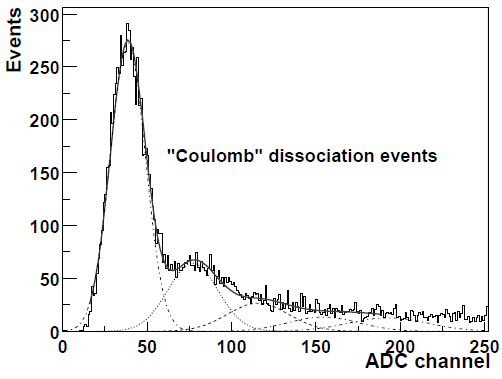
\includegraphics[width=.65\textwidth]{neuSpecRHIC}
    \caption{ZDC neutron spectrum at RHIC with each a Gaussian fit 
       to the 1, 2, 3, 5, and 5 neutron peak \cite{upcNeuPHENIX}.}
    \label{fig:neuSpecRHIC}
  \end{figure}
  Figure~\ref{fig:neuSpecRHIC} shows the charge recorded by the ZDCs.
  The peak at $\sim 30$ in Fig.~\ref{fig:neuSpecRHIC} is due to emission of a 
    single neutron. 
  Each successive peak is due to emission of an additional neutron. 
  From these peaks, the cross section for nuclear break-up by neutron 
    emission by both nuclei was measured.
  The fraction of nuclear interaction in all events with neutrons on both sides
    of the interaction point was found to be 0.661 $\pm$ 0.014 \cite{upcNeuPHENIX},
    which is in agreement the value 0.659 predicted by the model described in 
    \cite{emPCite4}.

  Nuclear collisions were separated from photon-induced break up by counting
    hits in the central scintillating counter similar to a tracker. 
  Events with hits on both sides of the interaction point were categorized as
    nuclear interactions, and those with no hits or hits on only one side were
    categorized as electromagnetic interactions. 
  The difference in the charge measured on each of the two sides of the 
    interaction point, by the two ZDCs, is divided by the total charge
    for both ZDCs (see Fig.~\ref{fig:neuRHICEMvHad}).
  \begin{figure}[!Hhbt]
    \centering
    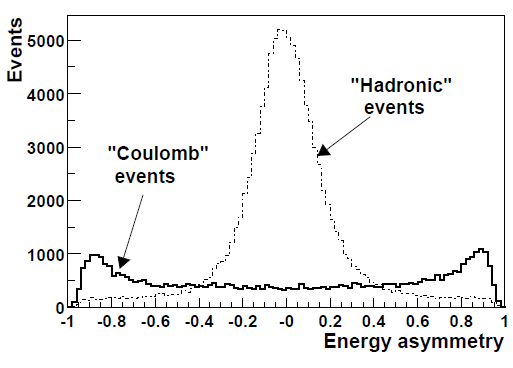
\includegraphics[width=.65\textwidth]{neuRHICEMvHad}
    \caption{The energy asymmetry in the ZDCs for photon-induced interaction, 
      coulomb events, and nuclear interaction, hadronic events \cite{upcNeuPHENIX}.}
    \label{fig:neuRHICEMvHad}
  \end{figure}
  Figure~\ref{fig:neuRHICEMvHad} shows that events created by electromagnetic 
    interactions result in asymmetric neutron emission, whereas nuclear 
    interactions produce neutrons on both sides. 
  In the analysis presented in this thesis, the energy asymmetry in the ZDCs is
    used to select UPC events.
  This will be discussed in Chapter~\ref{ch:triggChp}.


    \subsection{ UPC vector mesons photoproduction at RHIC }

    Both the $\rho^{0}$ and \JPsi{} meson photoproduction cross sections in UPC 
      events were measured at RHIC.
    STAR measured the photoproduction of the $\rho^{0}$ meson at collisions 
      energies per nucleon of 62.4 GeV \cite{upcRhoSTAR12}, 130 GeV 
      \cite{upcRhoSTAR02}, and 200 GeV \cite{upcRhoSTAR08}. 
    The \JPsi{} was measured by PHENIX at 200 GeV \cite{upcJPsiPHENIX}.
    The $\rho$ measurements by STAR were in good agreement with the theory
      calculation method described in Section~\ref{sec:vdmTheory}.
    The \JPsi{ } measurement where limited by statistic as only 10 \JPsi{}
      candidates were found. 

  \subsection{ UPC \JPsi{} at the LHC}
    The increase in beam energy from 200 GeV at RHIC to 2.76 TeV at the LHC 
      results in an increase in the Lorentz $\gamma$ of about 10.
    Because the photon flux depends on $\gamma^{2}$, the photon flux
      at the LHC increases by a factor of about 100 compared to RHIC.
    All major heavy ion experiments, ALICE and CMS, have studied the production
      of UPC events. 
    ALICE has studied coherent \JPsi{} photoproduction in ultra-peripheral PbPb
      collisions at $\sqrt{s_{NN}}$ = 2.76 TeV. 
   The cross section for this process was measured at both forward-rapidity, 
      $y$ = 3, and mid-rapidity, $y$ = 0.
   With an integrated luminosity of 55 $\mu$$b^{-1}$, ALICE measured 
     78 $\pm$ 10(stat) $^{+7}_{-11}$(syst) coherent \JPsi{} candidates at 
     forward rapidity.
   The measured cross section was 1.00 $\pm$ 0.18(stat) $_{-0.26}^{+0.24}$ 
    (syst) mb.
   For a symmetric system like PbPb collisions, as opposed to pPb collisions, 
    there is an ambiguity between which ion is the target and which is the 
    photon emitter. 
  Therefore, the cross section has a contribution from the low-$x$ and high-$x$ 
    parts of the gluon density. 
  At $y$ = 3  for PbPb collisions at the LHC, the cross section has a 
    contribution from both $x$ = 5 $\times 10^{-5}$ and $x$ = 2  $\times 
    10^{-2}$.
  This ambiguity is not present at $y$ = 0.
  ALICE has also measured the coherent \JPsi{} photoproduction cross section 
    at $y$ = 0, using a integrated luminosity of about 23 $\mu$$b^{-1}$.
  291 $\pm$ 18 (stat)$\pm$ 4(syst) and 265 $\pm$ 40 (stat)$\pm$ 12(syst) 
    coherent \JPsi{} candidates were measured in the dimuon and dielectron
    channels, respectively. 
  The combined cross section from both channels was measured to be 
    2.38 $_{-0.24}^{+0.34}$ (stat+syst) mb. 
  At $y$ = 0 $x$ $\sim$ 10$^{-3}$, which is a smaller $x$ than at forward 
    rapidity, and more sensitive to the nuclear gluon shadowing 
    (see Fig.~\ref{fig:aliceMoney}).
    \begin{figure}[!Hhbt]
      \centering
      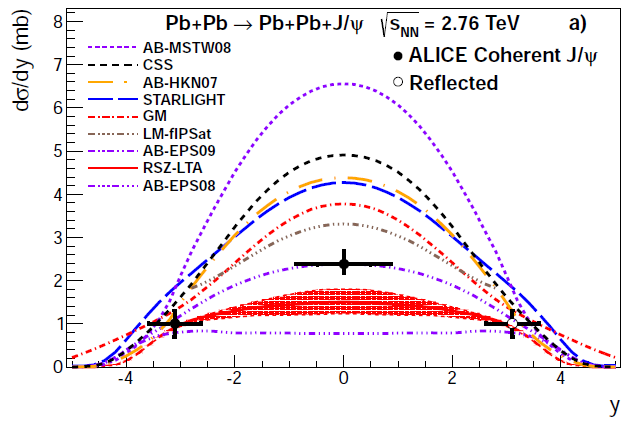
\includegraphics[width=.65\textwidth]{aliceJpsiCo}
      \caption{Coherent \JPsi{} photoproduction cross section in ultra-peripheral
        PbPb collisions at $\sqrt{s_{NN}}$ = 2.76 TeV, measured by the ALICE 
        experiment at forward and mid-rapidity \cite{}.}
      \label{fig:aliceMoney}
    \end{figure}

    The ALICE data points have been compared to several theoretical models. 
  The UPC photoproduction cross section calculations depend significantly on 
    how the nucleus is represented in the calculation. 
  The results from the STARlight, LTA, and AB methods vary from a relatively 
    large cross section in the STARlight model, ranging through a variety of values
    in the AB method, to a relatively small cross section in the LTA method. 
  Each of these methods utilizes the same probe of the nucleus, the equivalent 
    photon flux that is calculated using the Weizs\"{a}cker-Williams approximation 
    (see Section~\ref{sec:wwAprox}). 
  The three methods deviate in how they calculate the forward photoproduction
    scattering cross section.
  The differences in the UPC photoproduction cross sections predicted by the 
    different models demonstrates the amount of experimental sensitivity there 
    is to distinguishing between the models. 
  The dependence of the cross section on rapidity is clearly visible.   

  The cross section value calculated by Eq.~\ref{eq:finalSTARlightResult} in the 
    STARlight, LTA, and the various gluon density models in AB method vary 
    significantly.
  Table~\ref{tab:allXsec} gives the predicted values for the three main methods
    taken from \cite{pQCD2013.02}, \cite{lta2011.09}, and \cite{vmd1999}.
  \begin{table} 
   \centering
   \begin{tabular}{|l|l|} 
     \hline
     Model & $\sigma_{AA\rightarrow AAJ/\psi} (mb)$ \\ \hline \hline
     STARlight/STARlight MC & 23 \\ \hline
     LTA & 9 \\ \hline
     AB-MSTW08 & 34 \\ \hline
     AB-EPS08 & 7  \\ \hline
     AB-EPS09 & 14 \\ \hline
     AB-HKN07 & 23 \\ \hline
     \hline
   \end{tabular}
   \caption{$\sigma_{AA\rightarrow AAJ/\psi} (mb)$
    the LTA, STARlight, AB methods. Four different gluon density models are used 
    in the AB method. STARlight is a simulation software package that utilizes 
    the STARlight model.}
   \label{tab:allXsec}
  \end{table}
  The cross sections in Table~\ref{tab:allXsec} differ by a factor of 4 
    from the smallest to largest and create an experimental opportunity. 
  The clear discrepancy between the models in Table~\ref{tab:allXsec} 
    demonstrates the high amount of experimental sensitivity there is for 
    distinguishing between the models. 

  The nuclear suppression factor, S, demonstrates the difference between how 
    the models represent the nucleus. 
  $S$ is the ratio between the nuclear photoproduction cross section and the     
    free nucleon photoproduction cross seciton.
  It is a measure of how the nuclear gluon densities evolve in each of the 
    models. 
  Figure.~\ref{fig:ltaAndPqcdNucSub} from \cite{lta2013.05} shows the nuclear 
    suppression, which is equivalent to $R_g$ in Eq.~\ref{eq:ltaOptTheWNucMo}, 
    for the LTA and AB \DIFdelbegin \DIFdel{method}\DIFdelend \DIFaddbegin \DIFadd{methods}\DIFaddend .
  \begin{figure}[h] 
    \begin{center}
      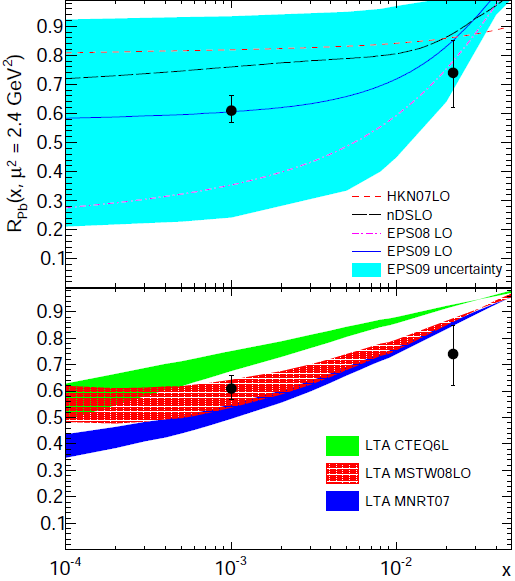
\includegraphics[width=0.5\textwidth,keepaspectratio]{ltaAndPqcdNucSub.png}
    \end{center}
    \caption{ \label{fig:ltaAndPqcdNucSub} Nuclear supression factor, $S$, in the AB and LTA methods.}
  \end{figure}
  \begin{figure}
    \begin{center}
      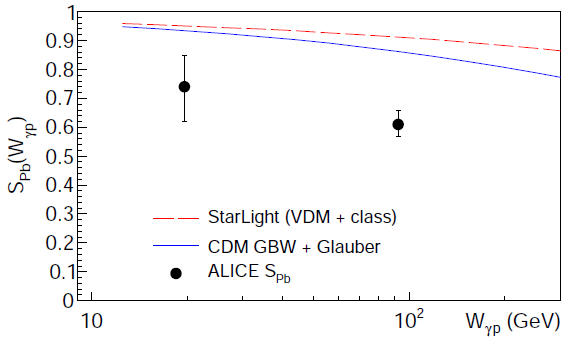
\includegraphics[width=0.5\textwidth,keepaspectratio]{ltaAndPqcdNucSubVMD.png}
    \end{center}
    \caption{ \label{fig:ltaAndPqcdNucSubSTARlight} Nuclear supression factor, $S$, in STARlight method.}
  \end{figure}
  Fig.~\ref{fig:ltaAndPqcdNucSubSTARlight} shows the nuclear suppression for the STARlight 
    method \cite{lta2013.05}. 
  Fig.~\ref{fig:ltaAndPqcdNucSub} and Fig.~\ref{fig:ltaAndPqcdNucSubSTARlight} 
    show that as the momentum of the probing photon goes up, increasing 
    $W_{\gamma p}$, and momentum of the probed gluon goes down, decreasing $x$, 
    the nuclear gluon density decreases relative to the free nucleon. 
  The nuclear suppression factor, $S$, allows for the different models' 
    representations of the gluon content of the nucleus to be directly compared
    to each other and to data. 
  $S$ can be measured from data by assuming a Weizs\"{a}cker-Williams photon flux and 
    provides insight into nuclear gluon densities.

  In addition, ALICE reported the measurement of the incoherent \JPsi{} 
    photoproduction cross section at mid-rapidity.
  This provided additional constraints to the models for gluon shadowing. 

  In Chapter~\ref{ch:analysis}, the coherent UPC \JPsi{} photoproduction 
    cross section using CMS is described.
  The measurement in this thesis adds to existing ALICE results, covering
    an intermediate range of $x$ values. 

  \chapter{\label{ch:detector} The Compact Muon Solenoid detector}	
  The Compact Muon Solenoid (CMS) is housed at interaction point 5 of the 
    LHC. 
  The LHC is designed to pursue physics at the TeV scale. 
  This is the scale where electroweak symmetry breaking is believed to occur
  	\cite{CmsPTdrv2}.
  While the search for the standard model Higgs boson was the 
    central driving design consideration, the wide range of possibilities for
  	finding new physics signals requires a general purpose detector.
  CMS was optimized \DIFdelbegin \DIFdel{to make excellent measurements of muons}\DIFdelend \DIFaddbegin \DIFadd{for efficient muon triggering and identification}\DIFaddend . 
  Muon capabilities developed for the Higgs boson \DIFaddbegin \DIFadd{studies }\DIFaddend can be used to study 
    \JPsi{}. 
  A versatile trigger is needed to accommodate the high interaction rates that 
    accompany the high luminosities. 
  By exploiting the versatility of the trigger and muon systems it
    is possible to explore processes like UPC \JPsi{} production, 
    which push to the low energy edge of the experiment's capabilities. 
  \begin{figure}[h]
    \centering
      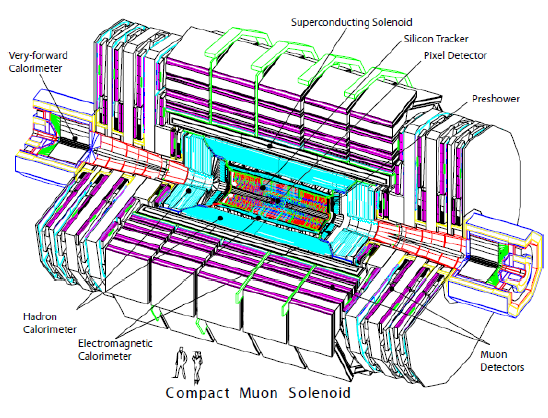
\includegraphics[width=.5\textwidth]{cms}
    \caption{The Compact Muon Solenoid layout \cite{tCmsE}.}
    \label{cms}
  \end{figure}

  CMS is dominated by the massive 4T 
  	superconducting solenoid at its core.
  The \DIFdelbegin \DIFdel{magnets }\DIFdelend \DIFaddbegin \DIFadd{magnet }\DIFaddend is 13m long with a 6m diameter, and pushes the limits of power
  	and compactness \cite{tCmsE}. 
  These two conflicting limits are achieved through the novel design of 
  	interweaving structural and conducting elements together in the coil of
  	the solenoid.

  Within the solenoid resides three different sub detectors.
  The \DIFdelbegin \DIFdel{inner most }\DIFdelend \DIFaddbegin \DIFadd{innermost }\DIFaddend is the world's largest silicon tracker \cite{tCmsE}.
  The tracker is surrounded by a highly effective lead tungstate crystal 
    electromagnetic calorimeter (ECAL)~\cite{CMS:2002xia}.
  ECAL is encapsulated in a brass scintillating hadronic calorimeter (HCAL).
  Outside the magnet, muon chambers are used to aid in the measurement and 
    triggering of muon events. 
  Altogether CMS weighs 12,500 metric tons, has a diameter of 14.6m,
    and a length of 21.6m \cite{tCmsE}.

  \section{Tracker}
    The Silicon Tracker~\cite{CMS:2000aa} is the innermost sub-detector of CMS, and has active
    	elements as close as 4.4cm to the interaction point \cite{tCmsE}. 
    The tracker has a length 5.8m, a diameter of 2.6m and
    	covers a range in pseudorapidity of $|\eta| <$ 2.5.
    At the center of the tracker are three rings of silicon pixels around the beam 
    	with two disks of silicon pixels to cap the rings.
    The pixel portion of the silicon tracker is comprised of 66$\times$10$^{6}$
    	pixels.
    The silicon pixels are surrounded by silicon strips.
    The silicon strips are separated into 4 different sections: 
    	the Tracker Inner Barrel, the Tracker Inner Disk, the Tracker Outer 
    	Barrel, and the Tracker End Caps.
    The silicon strip detectors as a whole are comprised of 9.3$\times$10$^{6}$ silicon 
    	strips.
    The high number of pixels and strips allow for the ability to distinguish
    	and collect enough distinct points to reconstruct the path of the 1000
    	or so charged particles per bunch crossing expected at peak luminosity
    	\cite{tCmsE}.
    \begin{figure}[!Hhbt]
      \centering
      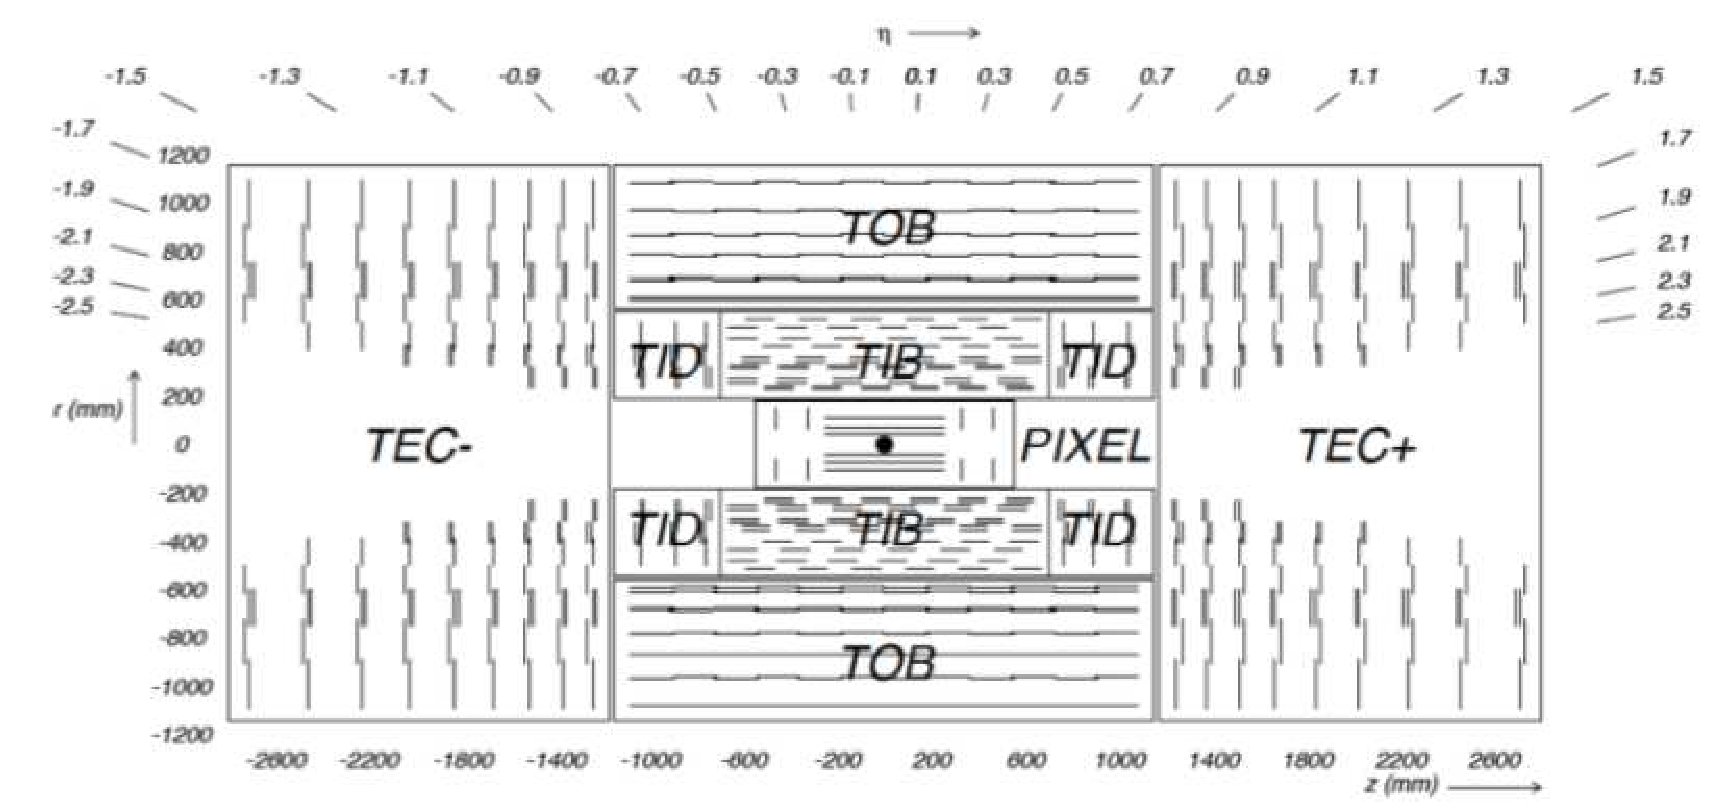
\includegraphics[width=0.75\textwidth]{trackerLayout}
      \caption{Layout of the silicon tracker with the pixels closest to the 
        interaction point, marked with a black dot, and the strips segments 
        beyond the pixels.}
      \label{fig:fig:trackerLayout}
    \end{figure}

    The amount of material present in the tracker is substantial enough to
      alter the path of particles as they pass through the tracker. 
    Fig.~\ref{fig:matBudge} shows the amount of material in the tracker 
      as a function of radiation lengths ($X_{0}$).
    A radiation length is the mean distance a photon travels before 
      interacting. 
    \DIFdelbegin \DIFdel{As opposed to the }\DIFdelend \DIFaddbegin \DIFadd{The }\DIFaddend deflection angle set by the strength of the magnetic 
      field \DIFdelbegin \DIFdel{, }\DIFdelend \DIFaddbegin \DIFadd{determines }\DIFaddend the momentum resolution for \DIFaddbegin \DIFadd{high momentum particles. 
    The momentum resolution for }\DIFaddend lower momentum tracks is limited by 
      the loss of energy due to multiple scattering of these particles off the 
      material of the detector.
    For UPC \JPsi{}, this is the primary factor contributing to the resolution 
      of the reconstructed muon tracks. 
    \begin{figure}[!Hhbt]
      \centering
      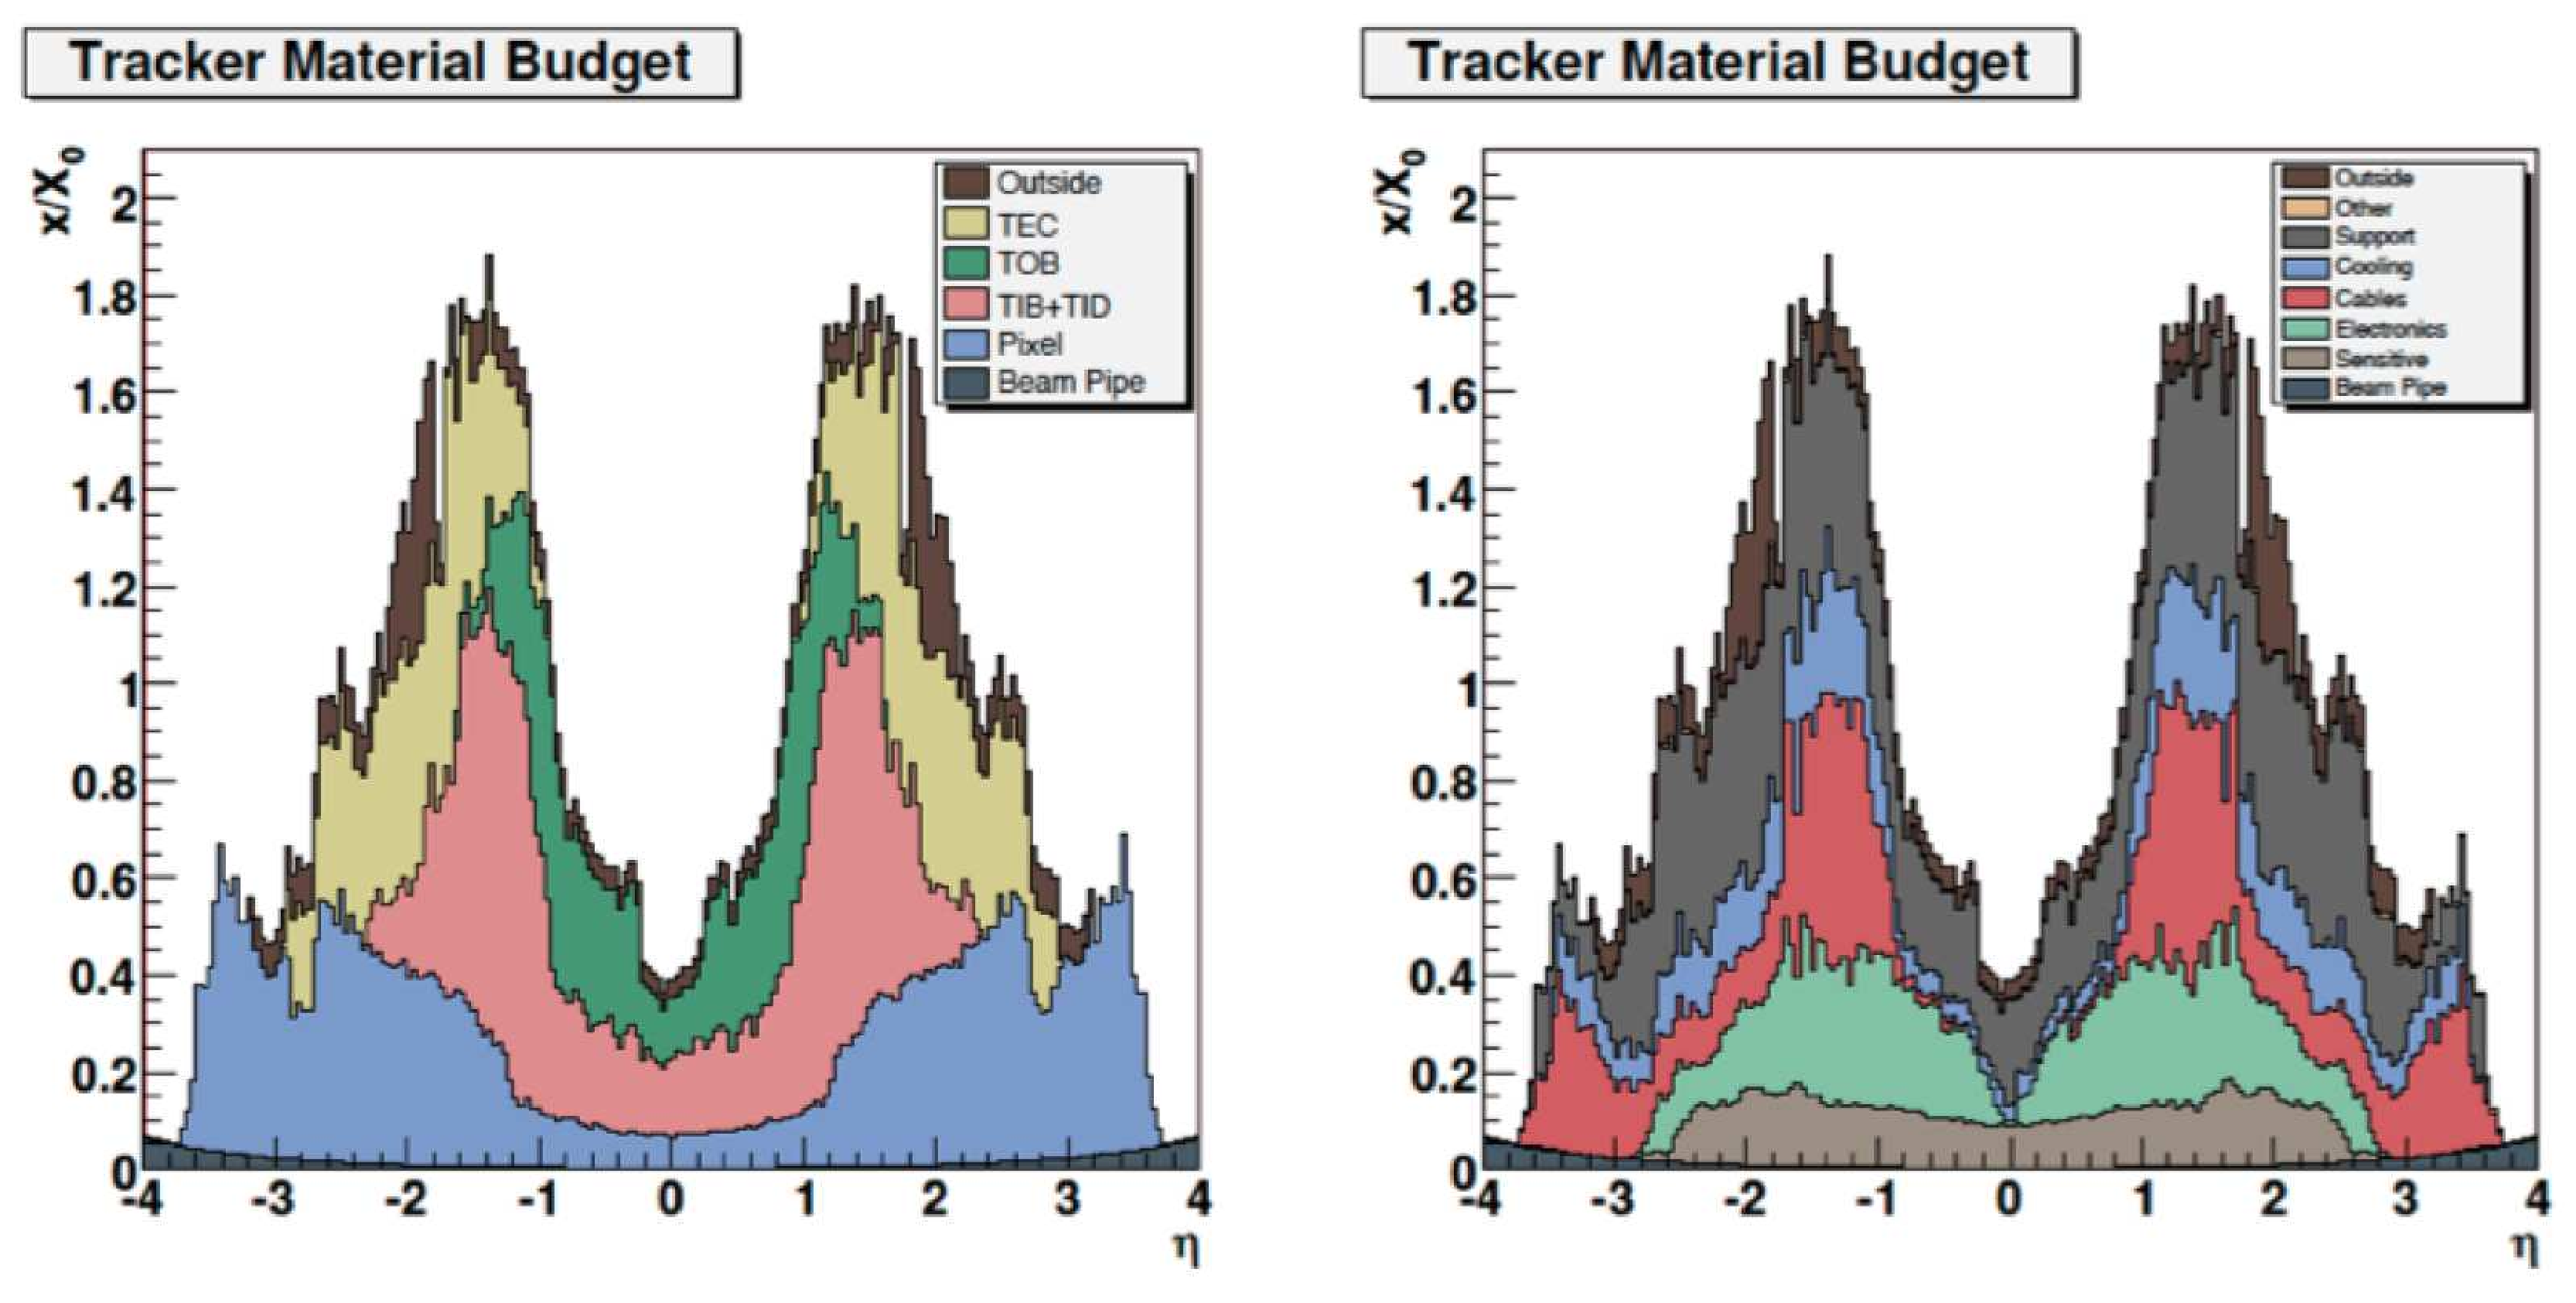
\includegraphics[width=0.65\textwidth]{matBudge}
      \caption{Material budget in the tracker broken down by sub-detector(left) and
        category (right)~\cite{tCmsE}.}
      \label{fig:matBudge}
    \end{figure}

  \section{ECAL}
    The next detector beyond the tracker is the electromagnetic calorimeter 
      system, ECAL.
    The calorimeter system is made of 61,200 lead tungstate (PbWO$_{4}$) 
      crystals in the central barrel and 7,324 in each of the two endcaps 
      \cite{tCmsE}.
    The barrel (EB) covers a pseudorapidity range $|\eta| < 1.479$ and has an
    	$\eta-\phi$ segmentation of approximately $0.0174\times0.0174$, depending
      slightly on the position of the fixed sized crystals.
    Lead tungstate is very dense giving the ECAL crystals a high number of 
      radiation lengths within a short depth.
    The crystals of the barrel have a depth of 230 mm corresponding to 25.8 
    	$X_{0}$.
    The endcaps (EE) cover the pseudorapitity region $1.479 < |\eta| < 3$.
    In the endcap the crystals have an exposed area of 28.62 $\times$ 28.62 
    	mm$^{2}$, and a depth of 220 mm corresponding to 24.7 $X_{0}$.
    The energy resolution of the ECAL as measured by test beam data can be seen in
    	Figure~\ref{ECALeRes}.
    \begin{figure}[!Hhbt]
      \centering
        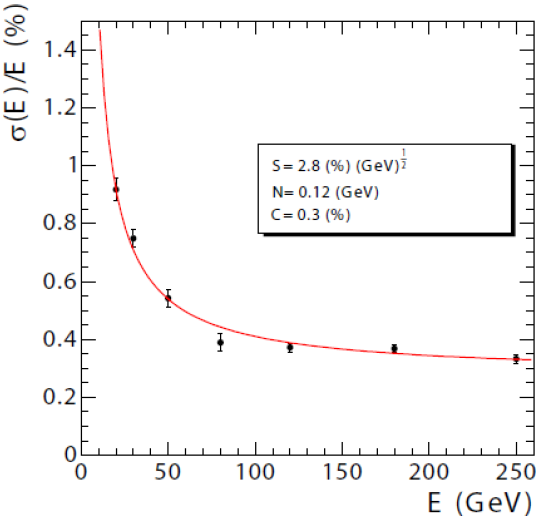
\includegraphics[width=0.5\textwidth]{ECALeRes}
      \caption{The energy resolution of ECAL as a function of energy~\cite{tCmsE}.}
      \label{ECALeRes}
    \end{figure}
    The fractional energy resolution reduces quickly above 10 GeV and levels
      off at about 0.5\% for energies above 100 GeV. 
    For \JPsi{} with rapidity near 2, the electron will carry energies around
      6 GeV and can be resolved by the ECAL. 

  \section{HCAL}
    The HCAL~\cite{Baiatian:2007xva} like the ECAL has both a barrel (HB) and endcaps (HE).
    The pseudorapidity region $|\eta|<1.3$ is covered by HB~\cite{tCmsE}. 
    HB has an $\eta-\phi$ segmentation of $0.0897\times0.0897$, and is 25 times more
    	sparsely granulated than EB.
    HE covers the pseudorapidity region $1.3<|\eta|<3$.
    HE, like EE and the tracker endcaps, is aligned parallel to the beam axis
    	resulting in granularity that changes with $\eta$.
    In the region $1.3 <|\eta|< 1.6$ HE has an $\eta-\phi$ segmentation of 
    	$0.0897\times0.0897$.
    The $\eta-\phi$ cell size roughly doubles to $0.17\times0.17$ in the region
    	$1.6 <|\eta|< 3$.
    The energy resolution of the barrel and endcaps can be seen in  
    	Figure~\ref{HCALeRes}.
    The thickness of the hadronic calorimeter is best described in interaction
    	lengths, $\lambda_I$, which is the mean distance a hadron travels before 
       it experiences a nuclear interaction.
    At $\eta = 0$ the barrel has a thickness 5.82 interaction lengths 
    	($\lambda_{I}$), and increases as the path length through the material 
    	increases to 10.6 $\lambda_{I}$ at $|\eta| = 1.3$.
    \begin{figure}[h]
      \centering
        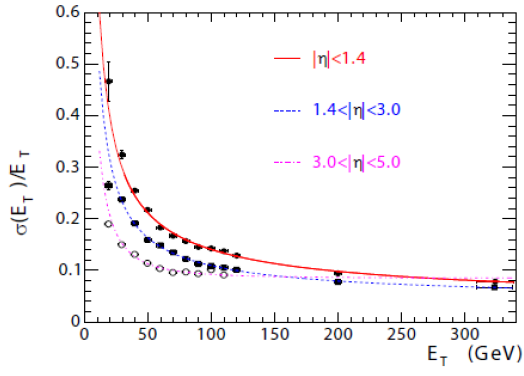
\includegraphics[width=0.5\textwidth]{HCALeRes}
      \caption{The $E_{T}$ resolution of HCAL as a function of $|\eta|$ and 
        $E_{T}$~\cite{tCmsE}.}
      \label{HCALeRes}
    \end{figure}

    In addition to HB and HE, HCAL has two additional calorimeters.
    Because the space between ECAL and the magnet is restricted to 1.18 m, an
    	outer hadronic calorimeter section (HO) is placed beyond the magnet
    	in the region $|\eta|<1.3$ \cite{tCmsE}.
    The main function of HO is to collect energy from the highest energy hadrons
    	before they reach the muon system.
    HO is not used in this analysis, but does contribute to the material budget. 
    To increase the total calorimetric coverage, HCAL also has a quartz fiber 
    	calorimeter (HF) in the forward region, $3 < |\eta| < 5$.
    For the majority of HF's 13 $\eta$ rings the $\eta-\phi$ segmentation is 
    	$0.175\times0.175$.
    In the lowest $|\eta|$ ring the segmentation is $0.111\times0.175$ in 
    	$\eta-\phi$.
    In the highest two $|\eta|$ rings the segmentation in $\phi$ is 0.349, with an
    	$\eta$ segmentation of 0.175 in the outer and 0.300 in the innermost 
    	ring. 
    The longitudinal direction is effectively segmented by using both short and
    	long fibers.
    The long fibers are sensitive to energy deposited throughout the calorimeter, i.e. to both the hadronic and electromagnetic parts of the shower. The short fibers are only sensitive to the energy deposited more than 22cm inside the calorimeter, which is mainly hadronic. 
    This allows electromagnetic showers to be distinguished from purely
      hadronic showers \cite{tCmsE}.

    The energy resolution for HF can be seen in Figure~\ref{HCALeRes}.  
    As with the ECAL, the fractional resolution increases with energy. 
    This is \DIFdelbegin \DIFdel{dues }\DIFdelend \DIFaddbegin \DIFadd{due }\DIFaddend to the random nature of shower development. 
    At larger energies, the fluctuations in the shower of particles collected 
      in the calorimeter tend to average out.

  \section{CASTOR}
   Very forward angles are covered at one end of CMS ($6.6 < \eta < 5.2$) by 
     the CASTOR calorimeter \cite{Andreev:2010zzb}.
   CASTOR is 1.6m long and 0.6m in diameter and sits 14.4m away from the nominal
     interaction point. It is 1.6m long and 0.6m in diameter. 
   CASTOR is a Cerenkov calorimeter made of quartz fibers/plates embedded in 
     tungsten absorbers.
   The quartz and absorbers are inclined at 40$^o$ to the beam axis to maximize
     the amount of Cerenkov light. 
   CASTOR is segmented into 16 $\phi$-sectors and 14 z modules.
   The two front modules comprise the electromagnetic section of the calorimeter
     with a depth of 20 radiation lengths. 
   Each of the electromagnetic channels has half the depth of the hadronic ones. 
   The total thickness  of CASTOR is about 10 interaction lengths. 

  \section{ZDC \label{sec:zdcDet}} 
    Beyond HF, the Zero Degree Calorimeters (ZDCs)~\cite{Grachov:2006ke} covers the very forward 
      rapidity region.
    The ZDCs sit between the beam pipes on either side of the interaction point 
      covering the area around $\theta = 0$, $|\eta| > 8.3$.
    In heavy ion collisions the ZDC has the ability to measure neutral particles 
    	that do not participate in the collision \cite{tCmsE}.
    This detector plays an important role in the analysis described in this
      thesis by measuring energy due to neutrons produced by photon-induced 
      nuclear break.
    These measurements are used to identify events with asymmetric neutron 
      emission, reducing the contribution to the sample by peripheral \DIFdelbegin \DIFdel{heavy-idon
}\DIFdelend \DIFaddbegin \DIFadd{heavy-ion.
      This will be discussed further in Chapter~\ref{ch:zdcReco}.
}\DIFaddend 

    The ZDC has a total of 18 channels.
        Half of these 18 channels are on either side of the interaction point.
    The 9 channels on the side of CMS that correspond to positive $\eta$
      are denoted ZDC$^{+}$, where as the 9 channels on the negative side are
      denoted ZDC$^{-}$.
    The 9 channels on each side are further sub-divided into an electro-magnetic  
      (EM) section and a hadronic (HAD) section.
    The EM section is positioned in front of the HAD section with respect to the 
      interaction point and is segmented transverse to the beam direction.
    The 5 EM sections are positioned in front to absorb the energy from 
      electro-magnetically induced showers, which develop over a shorter distance 
      than hadronically induced showers.
    The transverse segmentation allows for a measurement of the transverse shower
      width and the size of the beam spot at the ZDC.
    The HAD section is segmented in the direction of the beam and consists of 4
      channels.
    The longitudinal segmentation allows for absorption of the full extended 
      hadronic shower and the ability to measure the longitudinal shower shape.

    Each of the 18 channels contains a tungsten target and quartz fibers.
    The dense tungsten target is used to initiate the shower.
    The quartz fibers shine Cerenkov light as the high momentum charged particles
      from the shower pass through it. 
    the light from the quartz fibers is channeled to photo-multiplier tubes, one 
      for each ZDC channel. 
    Through a cascade of photon induced electrical discharges, the photo-multiplier
      converts the Cerenkov light to an electrical pulse. 

    This electrical pulse travels $\sim$ 200 m down a coaxial cable from the LHC
      tunnel to the counting house in the CMS service cavern. 
    There the electrical pulse is digitized by the Charge Integrator and Encoder 
      (QIE).
    The QIE integrates the current each 25 ns.
    The charge is then mapped logarithmically to the 128 bits. 
    \DIFdelbegin \DIFdel{This bit is }\DIFdelend \DIFaddbegin \DIFadd{These bits are }\DIFaddend sent across a small fiber optic cable to the HTR firmware card.
    Here each 25 ns signal is stored in a 250 ns buffer, and the timing is synchronize
      with the rest of the detector to ensure the ZDC signal arrives at the central
      data acquisition system at the same time as the other sub detectors from the 
      same collision. 

  \section{Muons}
    The muon system~\cite{tCmsE} resides just outside of the superconducting magnet.
    It consists of three complementary systems: drift \DIFdelbegin \DIFdel{tube }\DIFdelend \DIFaddbegin \DIFadd{tubes }\DIFaddend (DT) in the
      barrel, cathode strip chambers (CSC) in the endcaps, and resistive 
      plate chambers (RPC) in both the barrel and endcap regions \cite{tCmsE}.
    Each of these gaseous detectors function in the same way.
    As the muon penetrates the gas volume electrons are knocked off of the 
      gas atoms and these electrons are collected in the positively charged
      anode, whereas the ionized gas moves to the cathode. 
    The DTs in the barrel and the CSCs in the endcap have better spatial 
      precision relative to the RPCs, which are quicker and have more
      precise timing. 
    The combination of the DTs and RPCs in the barrel and the CSCs and RPCs 
      in the endcap allow for fast triggering and muon identification during
      data reconstruction. 
    \begin{figure}[!Hhbt]
      \centering
      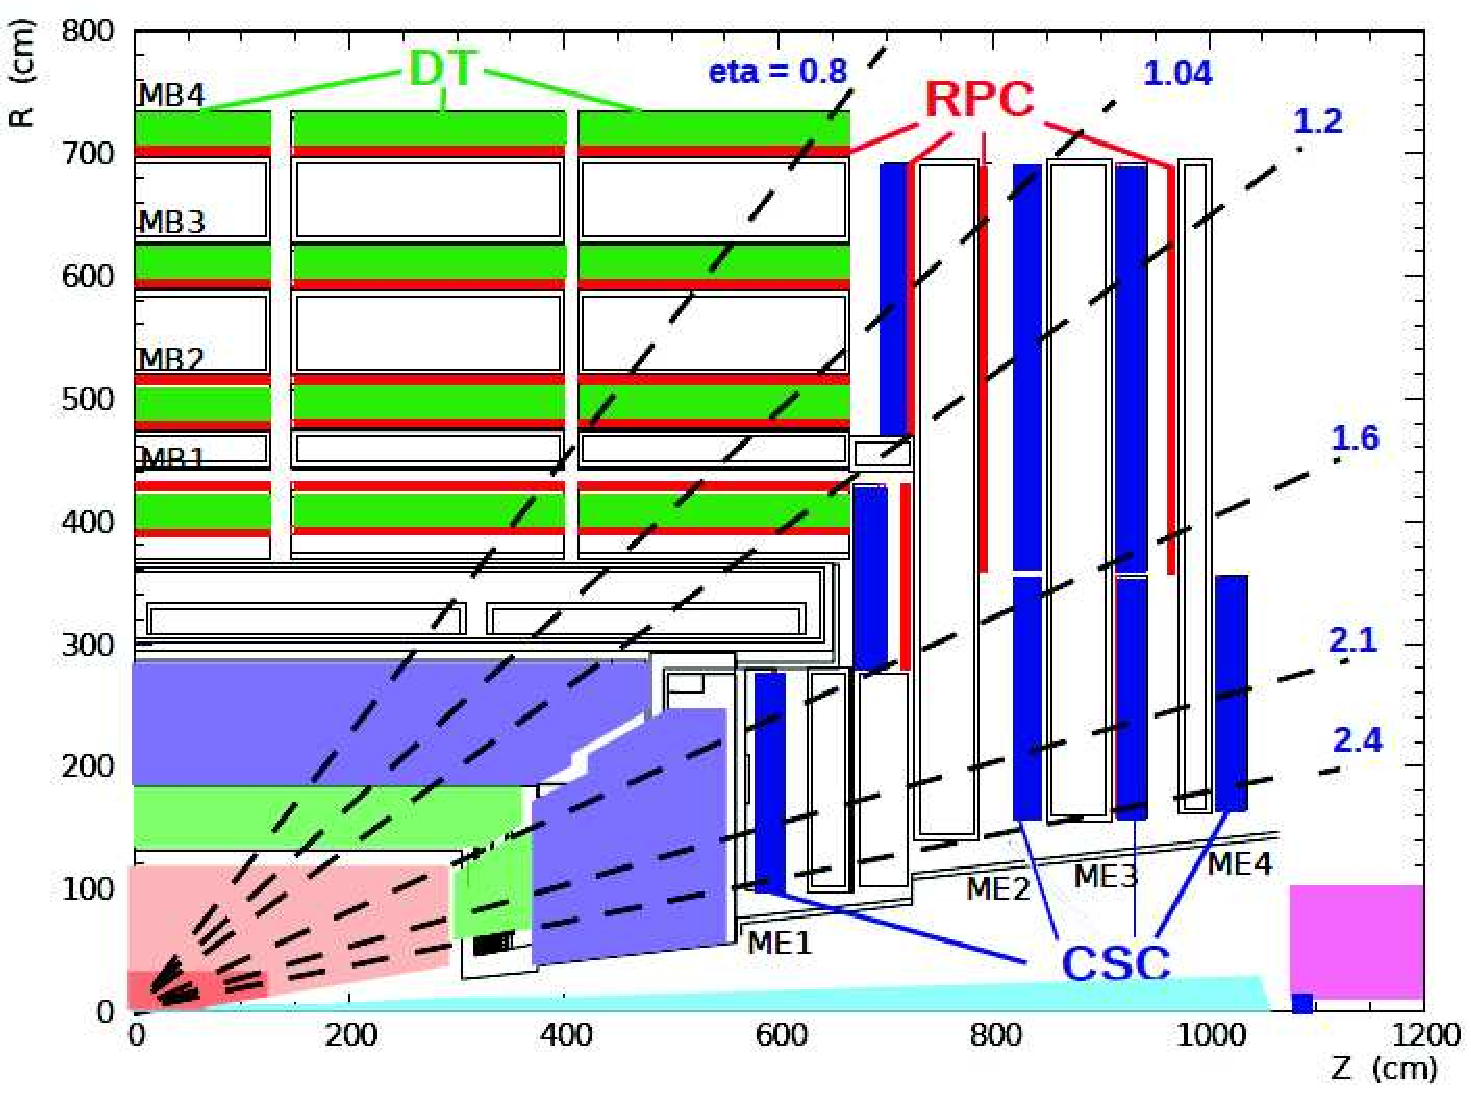
\includegraphics[width=.65\textwidth]{muonSys}
      \caption{ The CMS muon system showing the four DT stations in 
        the barrel (MB1-MB4), the four CSC stations in the endcap (ME1-ME4), 
        and the RPC stations.}
      \label{fig:muonSys}
    \end{figure}

    As seen in Fig.~\ref{fig:muonSys}, the DTs reside only in the barrel, 
      covering the region $|\eta|$ < 1.2.
    Consisting of a total of 172,000 cells, the DT cells are collected into
      250 chambers. 
    The DT chambers are in interwoven into the magnet field return yoke and are
      labeled by 5 segmentations in $z$, YB-2 to YB+2.
    Each $z$ segment is divided into 12 $\phi$ segments labeled 1 at $\phi$ = 0
      and going to 12 rotating in positive $\phi$ with segments 4 and 10 
      containing 2 chambers.
   The segmentation in $r$ is divided into four parts, MB1-MB4.
   Fig.~\ref{fig:dtSchem} shows how each chamber is made of three super layers.
   Super layers SL $\Phi_{1}$ and SL $\Phi_{2}$ measure $(r,\phi)$, whereas 
    SL $\Theta$ measures $z$.
    \begin{figure*}[!Hhbt]
      \centering
      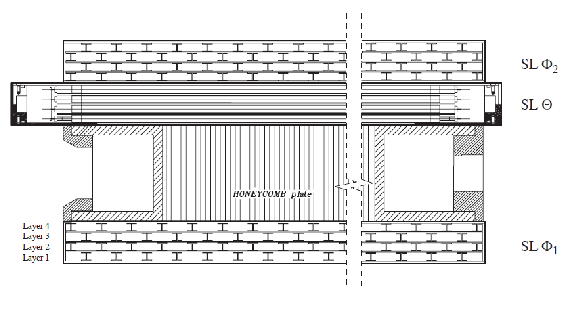
\includegraphics[width=.85\textwidth]{dtStruct} \\
      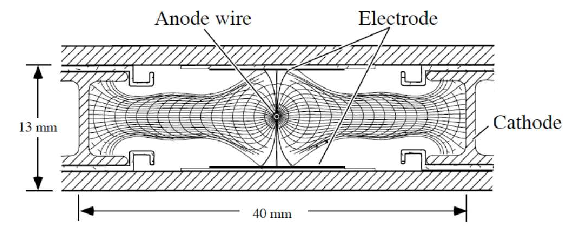
\includegraphics[width=.85\textwidth]{dtCell}
      \caption{Schematic of the DT chambers and an individual DT cell.}
      \label{fig:dtSchem}
    \end{figure*}

    The RPCs complement the DTs in the barrel and the CSCs in the endcap 
      primarily for the purpose of triggering.
    Throughout the barrel and endcap there are a total of 1020 RPC modules, 480
      in the barrel and 540 in the endcap.
    Denoted by the red lines in Fig.~\ref{fig:muonSys}, the RPCs are mounted on
      both sides of the DTs in the barrel for the inner most layers, MB1 and 
      MB2.
    For the outer two layers of the barrel, MB3 and MB4, a single layer of RPCs
      is mounted on the inner side of the DTs.
    Each corresponding DT segment has two RPCs modules, \DIFdelbegin \DIFdel{expect }\DIFdelend \DIFaddbegin \DIFadd{except }\DIFaddend in MB2 where 
      some segments contain 3 RPC modules. 
    The outer ring of the muon endcaps are instrumented with RPCs covering up to
      $|\eta|$ = 1.6.
    \begin{figure}[!Hhbt]
      \centering
      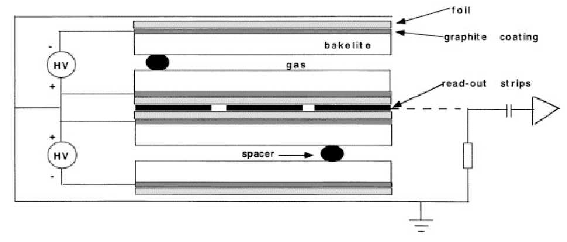
\includegraphics[width=.65\textwidth]{rpcCell}
      \caption{Schematic of a RPC cell.}
      \label{fig:rpcSchem}
    \end{figure}

    There are a total of 468 CSC modules in the muon system endcap. 
    For the sectors in $z$, ME2, ME3, and ME4 in the endcap, the modules in 
      the ring closest to the beam cover 20$^{\circ}$ in $\phi$.
    The modules in ME1 and the modules beyond the inner ring in
      ME2 and ME3 have a 10$^{\circ} \phi$ segmentation.
    The 2 million wires of the CSCs are grouped into 400,000 channels and are
      powered with 9000 high voltage supplies. 
    The resolution of the CSCs in on the order of 1mm for position measurements 
      in the plane perpendicular to the beam and they are 99\% efficient for muons
      that pass through all four sectors, ME1, ME2, ME3, and ME4.
    Because of the relatively low momentum of the muons originating from \JPsi{}
      in UPC events, the muons in the analysis discussed in this thesis are all
      in the range $1.6 < |\eta| < 2.4$ and rely on the CSCs for triggering. 
    \begin{figure}[!Hhbt]
      \centering
      $ \begin{array}{cc}
        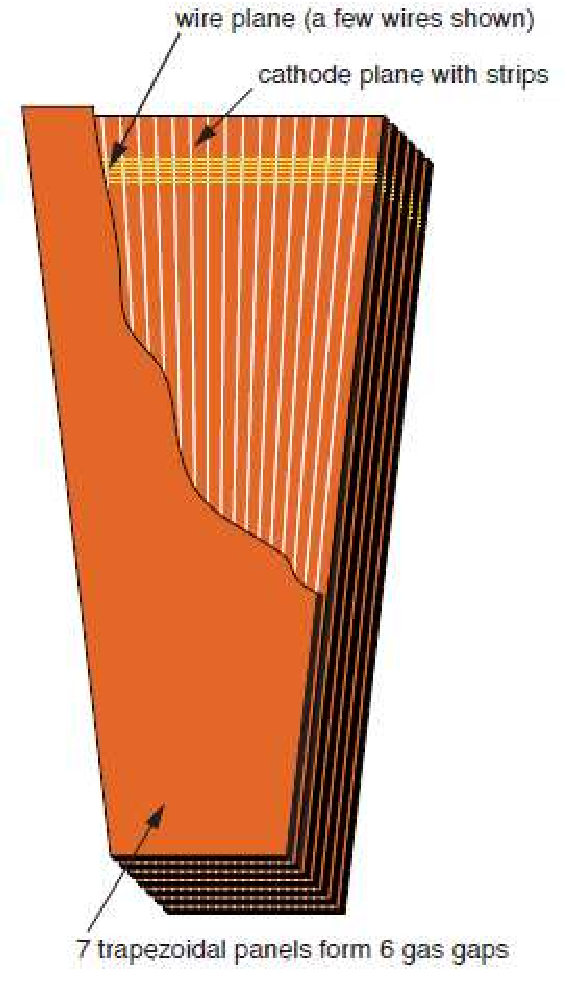
\includegraphics[width=.35\textwidth]{cscStruct} &
        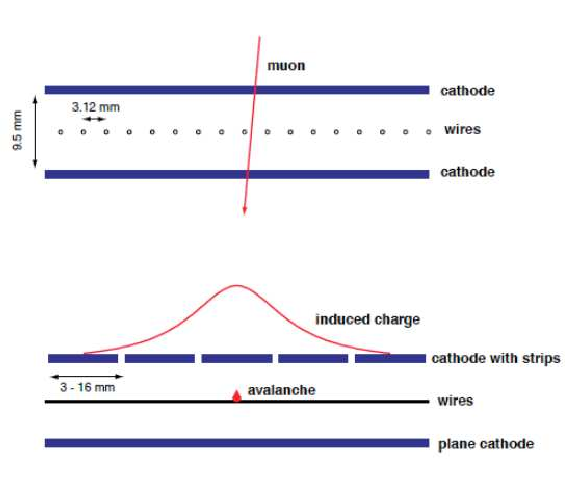
\includegraphics[width=.65\textwidth]{cscCell}
      \end{array} $
      \caption{Schematic of the CSC chambers and an individual CSC cell.}
      \label{fig:cscSchem}
    \end{figure}

    The primary function of the muon systems is to trigger on and identify 
      muons.
    The tracker is still the primary instrument for measuring the muons. 
    Fig.~\ref{fig:muonRes} shows that the muon system only improves the 
      momentum resolution for muons with momenta above 100 GeV. 
    For UPC \JPsi{}~events, where muons momenta are between 4-8 GeV, the muon
      system does not provide any advantage in terms of improved resolution.
    The muon system is however important in distinguishing which tracks are 
      due to muons as opposed to other charged particles.
    Because of their much larger mass relative to electrons, muons emit less 
      bremsstralung, or breaking radiation, as they penetrate the inner layers
      of the CMS on its way to the muon systems.
    Fig.~\ref{fig:matThick} shows the amount of material traversed by particles
      traveling through CMS as a function of $|\eta|$.
    The total of nearly 10 interaction lengths between the interaction point 
      and the muon chambers ensures that hadrons like charged poins, which
      almost exclusively decay to muons, are absorbed in the calorimeters 
      before converting to muons. 
    By eliminating backgrounds from both electrons and hadrons, the CMS muons 
      system allows for identification of muons for both triggering and 
      reconstruction.
    \begin{figure}[!Hhbt]
      \centering
      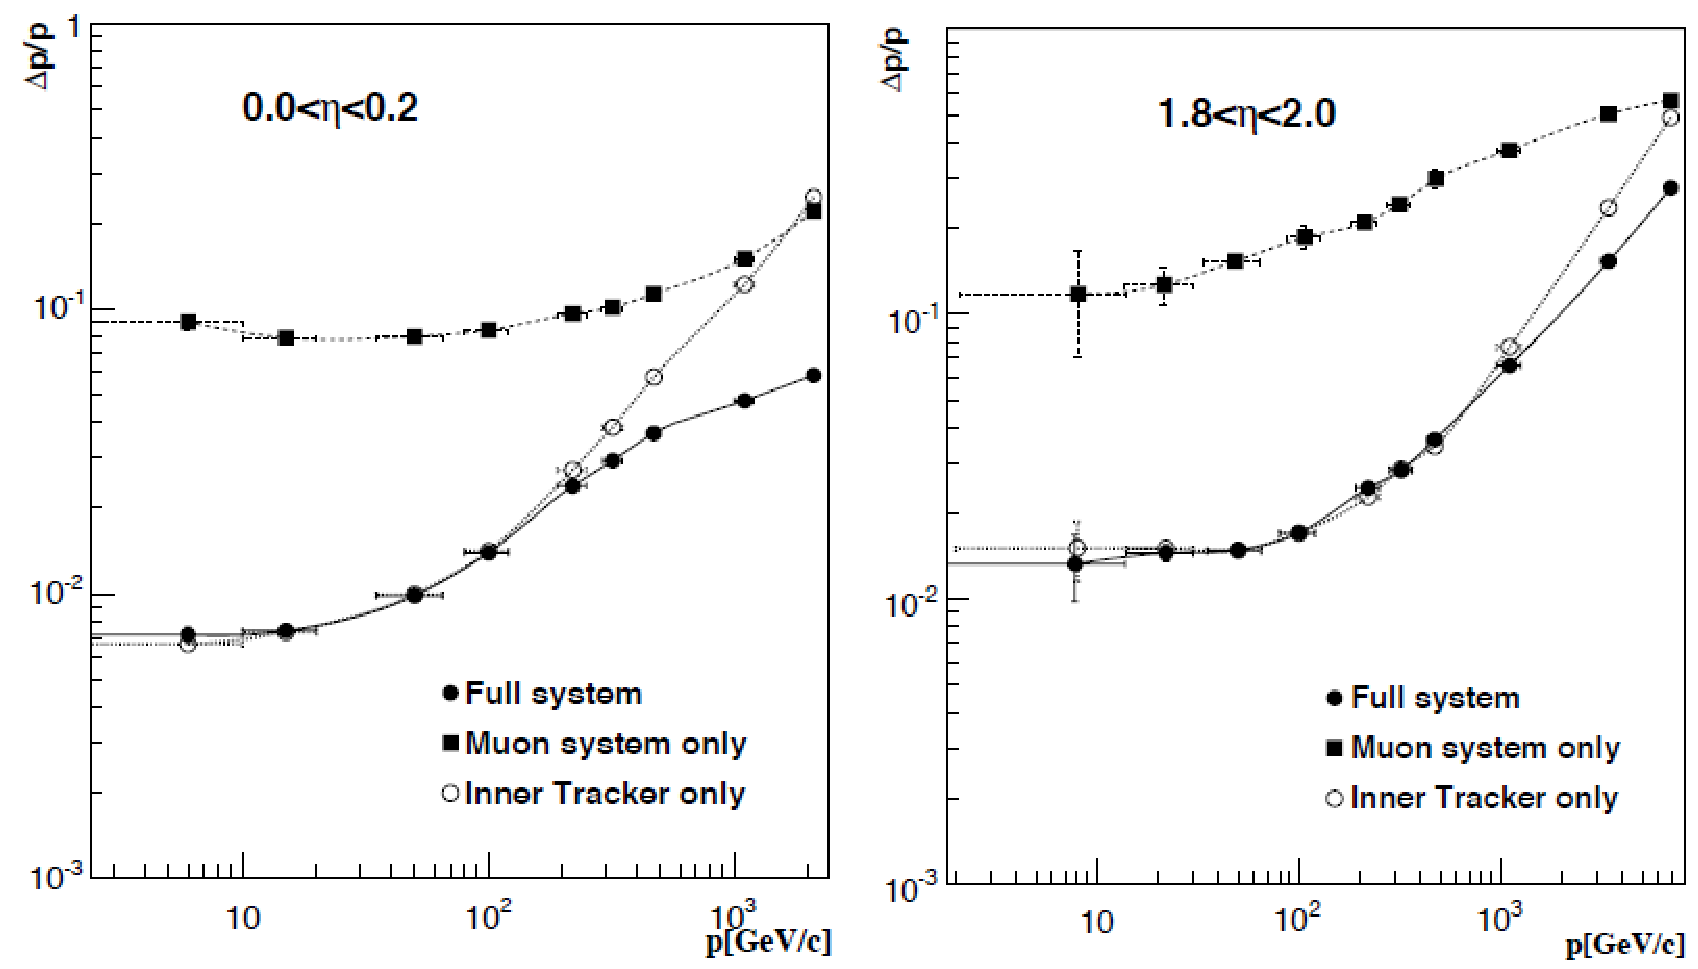
\includegraphics[width=.65\textwidth]{muonRes}
      \caption{ The momentum resolution for muons using only the 
        tracker and the whole muon system in the barrel (left) and end cap 
        (right)~\cite{tCmsE}.}
      \label{fig:muonRes}
    \end{figure}

    The low-momentum nature of UPC physics creates complications due to the 
      large amount of material between the interaction point and the muon 
      systems.
    About 3 GeV of momentum is needed to reach the first layers of the muon 
      system.
    In the rest frame of the \JPsi{}, the \JPsi{} equally shares its rest mass with 
      its decay products creating 2 muons with momenta of about 1.5 GeV.
    For these daughter muons to reach the muon system, their parent \JPsi{} must
      be pushed to higher momentum by the initial particles which created the
      \JPsi{}.
    For this reason, muons from UPC \JPsi{}s are only detected at higher 
      $\eta$ values.
    Understanding this momentum restriction of the muon system was a major 
      focus of the analysis discussed in this thesis with details described in 
      Section.~\ref{sec:effDet}.
    \begin{figure}[!Hhbt]
      \centering
      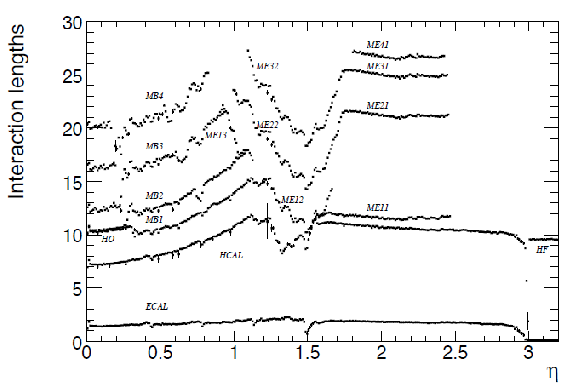
\includegraphics{materialThickness}
      \caption{The amount of material in CMS as a function of $\eta$ in 
        number of interaction lengths~\cite{tCmsE}.}
      \label{fig:matThick}
    \end{figure}

  \section{\label{sec:detTrg}Trigger}
    The CMS trigger is two tiered~\cite{Dasu:2000ge,Sphicas:2002gg}. 
    The L1 trigger is the lower level hardware based system. 
    The High Level Trigger (HLT) is a software base and runs on a computer farm
      located at point 5.

    The purpose of the L1 trigger is to make quick decisions about which events
      will be kept temporarily for further processing.
    It uses only information from the calorimeter and muon systems and is used
      to identify events where the tracker should be read out.
    The output from the sub-detectors is synchronized to ensure that the signal
      from each of the sub-detectors comes from the same collision. 

    If an event passes the L1 trigger, the data from all the sub-detectors,
      including the tracker are sent to the HLT computing farm. 
    At this level the raw data from all the sub-detectors is unpacked and 
      combined.
    The information from the calorimeters, muon system, and tracker can all 
      be used to reconstruct basic physic objects in the HLT farm. 
    For example, tracks can be associated with either ECAL energy clusters to 
      form electron candidates, or tracks can be combined with hits in the muon
      system to create muon candidates.
    At the HLT, the whole detector is used to select events.
    The raw data from the events that survive the HLT are recorded permanently,
      those that do not are lost forever. 

    The HLT farm must always be ready to accept events from the L1 trigger.
    For this reason, the amount of computing time each HLT trigger path uses
      must be balanced.
    For more rare L1 triggers, which will occur at a lower rate, more 
      complex reconstruction software can be used.
    Conversely, simpler, faster, methods must be used for more common high
      rate triggers. 
    Because of this time constraint in the HLT farm, the reconstruction 
      algorithms used for triggering tended to differ from the final 
      reconstruction algorithms.
    In the HLT these algorithms are optimized for quickness, whereas the final 
      reconstruction is optimized for precision and accuracy.
    By having the ability to spend different amounts of computing time on 
      different L1 triggered events, the complexity of the event selection 
      offered by the HLT is heightened. 

    The two tiered triggering system creates very low dead times while 
      maintaining purity and selectivity.
    The wide gamete of physics topics that are pursued by the CMS collaboration
      are a testament to the effectiveness and versatility of the CMS two 
      tiered triggering system.
    In Chapter~\ref{ch:trigg}, the development of L1 triggers and HLT paths 
      for selecting UPC \DIFdelbegin \DIFdel{evens is }\DIFdelend \DIFaddbegin \DIFadd{events are }\DIFaddend discussed. 

  \chapter{\label{ch:zdcReco}ZDC reconstruction}
  \section{\label{sec:breakUpDet} Nuclear break-up determination}
    As described in Section~\ref{sec:ltaTheory}, UPC \JPsi{} photoproduction 
      can be accompanied by the emission of neutrons from either of the two 
      colliding nuclei.
    The various neutron emission scenarios, or break-up modes, can 
      be distinguished by the two ZDCs.
    By separating events where the ZDC signal is consistent with 1 neutron 
      versus several neutrons, or where neutrons are present on only one or 
      both sides, the fraction of events which corresponds to a given 
      break-up mode can be measured and compared to theory. 

    In order to maximize the ability to explore the one neutron peak, which 
      sits at the bottom of the ZDCs dynamic range, a new ZDC reconstruction 
      method was devised. 
    This new reconstruction method was then used to establish 
      thresholds for one and more than one neutron in each ZDC. 
    This section describes the ZDC signal reconstruction and how the neutron 
      thresholds on this signal were set.

    \subsection{ZDC signal reconstruction}
      The signal from each ZDC is built up from the pulse shapes for each of 
        the 18 individual ZDC channels. 
      The pulse shape is recorded in 250 ns second chunks and is divided into
        10 time slices of 25 ns (see Fig~\ref{fig:zdcPulseShape}).
      Counting from 0, the 4th time slice is synced with the timing of the rest
        of the detector and corresponds to when the products of the recorded 
        collision reached the ZDC.
      The signal is therefore taken from the 4th time slice.
      \begin{figure}[h]
        \centering
        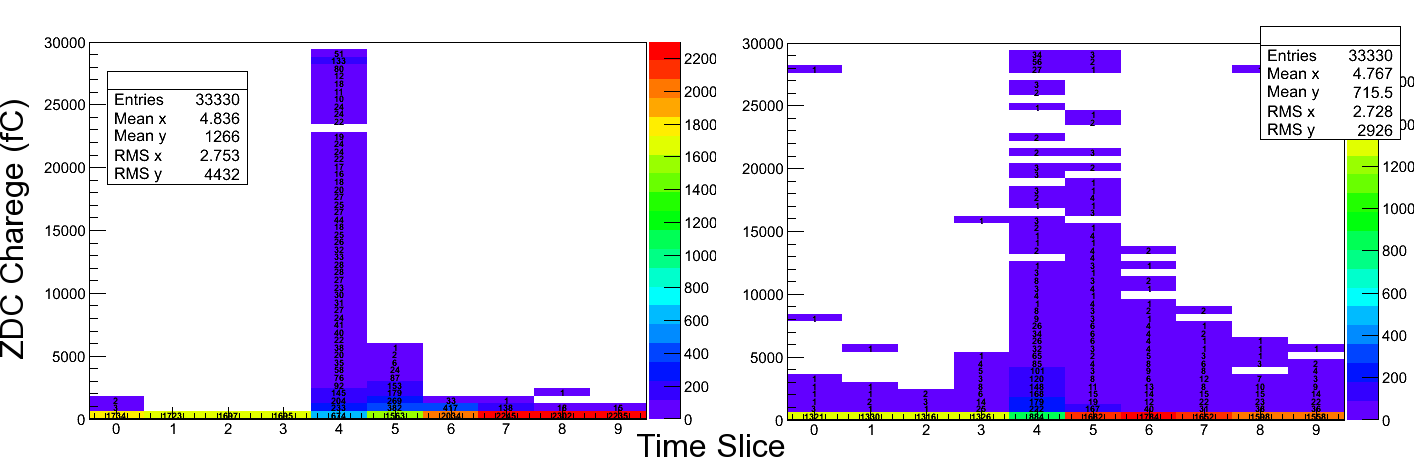
\includegraphics[width=\textwidth]{zdcPulseShape}
        \caption{Average ZDC pluse shape is plotted as the charge as a function
          of time slice for the first hadronic from ZDC$^{-}$ (left) and 
          ZDC$^{+}$ (right).}
        \label{fig:zdcPulseShape}
      \end{figure}

      The ZDC signal sits on top of a low frequency noise pedestal with a 
        period of about 2$\mu$ seconds. 
      Over the time scale of 250 ns, this low frequency noise signal appears
        as a constant that shifts randomly from event to event.
      The contribution from this noise is therefore measured event by event
        in order to subtract it.
      Time slice 5 is used for this purpose.
      Time slices 1 and 2 could also be used to estimate the low frequency 
        noise.
      However because the noise fluctuates to negative values of charge that 
        cannot be measured, these time slices can only provide a 
        measurement of the noise half the time. 
      By using time slice 5 which contains the falling tail of the signal, 
        the noise can be measured any time the signal raises significantly 
        above the noise.
      If the fraction of signal in time slice 4 and 5 are constant and
        the noise contributes the same value to both time slices, the 
        following formula is applicable:
      \begin{equation}
        Ts4 \propto (Ts4 + C) - ( Ts5 + C ) = Ts4 - R_{Ts5/Ts4}Ts4 
        = Ts4(1-R_{Ts5/Ts4}),
        \label{eq:ts4ish}
      \end{equation}
      where $Ts4$ is the signal contribution in time slice 4, $Ts5$ is the 
        signal contribution to time slice 5, $C$ is a random noise constant
        from the low frequency noise, and $R_{Ts5/Ts4}$ is the ratio between
        the signal contribution from time slice 5 over time slice 4.
      Figure~\ref{fig:zdcTs4OvTs5VTs5} demonstrates the consistency of the 
        fraction and validates the unconventional method of using the falling 
        tail of the signal to estimate the low frequency noise. 
      By using time slice 5, the chances of measuring the noise are maximized. 
      Separating the signal from the noise is especially important because
        the ZDC signal for the one neutron peak sits near the noise at the 
        bottom of the ZDC dynamic range.
      \begin{figure}[!Hhbt]
        \centering
        $ \begin{array}{cc}
          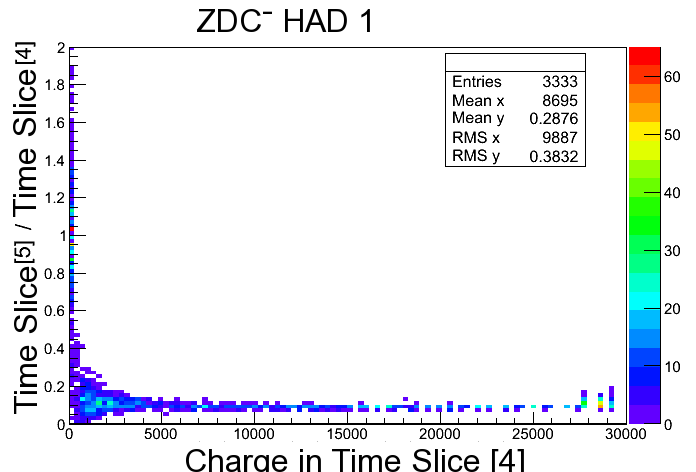
\includegraphics[width=.4\textwidth]{negTs5overTs4vts5} &
          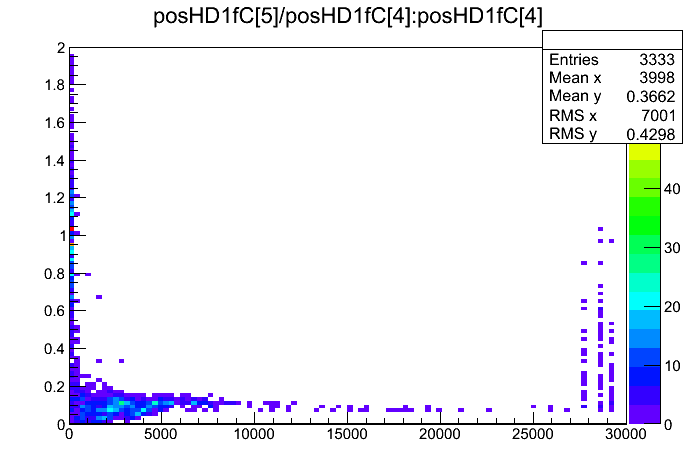
\includegraphics[width=.4\textwidth]{posTs5overTs4vts5}
        \end{array} $  
        \caption{ The fraction of signal in time slice 5 over time slice 4 
          as a function of the signal in time slice 5 in ZDC$^{-}$ (left) and 
          ZDC$^{+}$ (right).}
        \label{fig:zdcTs4OvTs5VTs5}
      \end{figure}

      When summing the 9 channels in each ZDC\DIFaddbegin \DIFadd{, }\DIFaddend only channels with signals above 
        zero in time slices 4 and 5 were included. 
      The EM, electromagnetic, section of the calorimeter is more densely 
        packed with quartz fibers and therefore has a higher gain relative to 
        the HAD, hadronic, section. 
      To account for this, the EM channels were weighted with
        a factor of 0.1 to match the HAD channel gains.

    \subsection{Determination of the one neutron thresholds}
      The ZDC thresholds used to establish the various break-up modes were 
        measured from zero bias data.
      Figure~\ref{fig:zdcM2Fit} shows the weighted sum of the EM and 
        HAD sections for  ZDC$^{-}$ and  ZDC$^{+}$ for the zero bias 
        dataset.
      The neutron spectrum for this dataset is not biased since the 
        trigger only required that both beams were present in CMS. 
      This dataset does, however, include a significant electronic noise contribution due
        to events where no neutrons are emitted in the direction of the ZDC.
      It is clear from Fig.~\ref{fig:zdcM2Fit} that the gain of  
        ZDC$^{+}$ is lower than that of ZDC$^{-}$. 
      This is because of a damaged phototube on the first HAD section 
        of ZDC$^{+}$.

      To determine the thresholds for one and multiple neutrons, the ZDC$^{+}$ 
        and ZDC$^{-}$ spectra were 
        each fit to the sum of four Gaussians. 
      The electronic \DIFaddbegin \DIFadd{pedestal }\DIFaddend noise was fit to a Gaussian around zero.
      The one, two, and three neutron peaks are fit to Gaussians that are 
        successively broader.
      The mean of each peak was initially set to multiples of the mean of the 
        one neutron peak. 
      \begin{figure}[!Hh]
        \centering
        $
          \begin{array}{cc}
            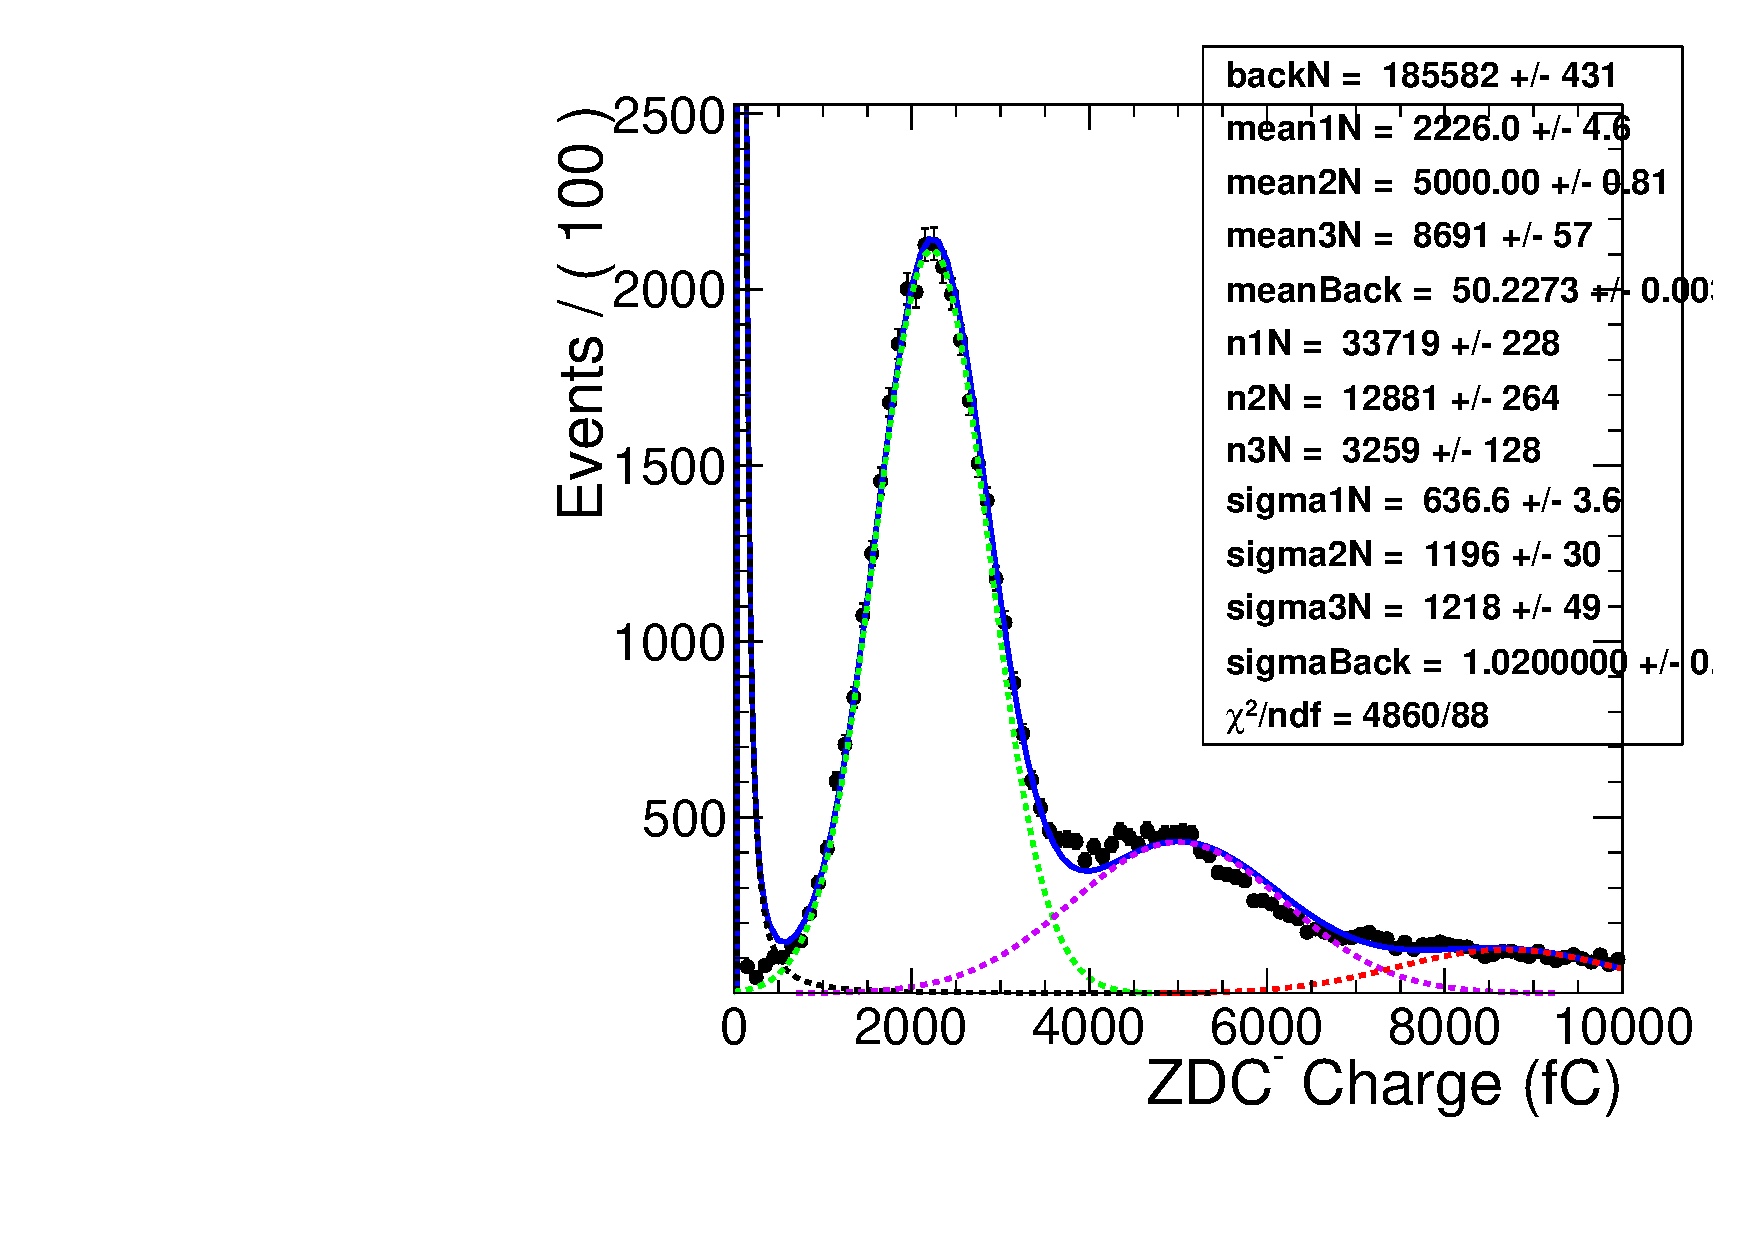
\includegraphics[width=0.45\textwidth]{zdcFit45Neg.pdf} &
            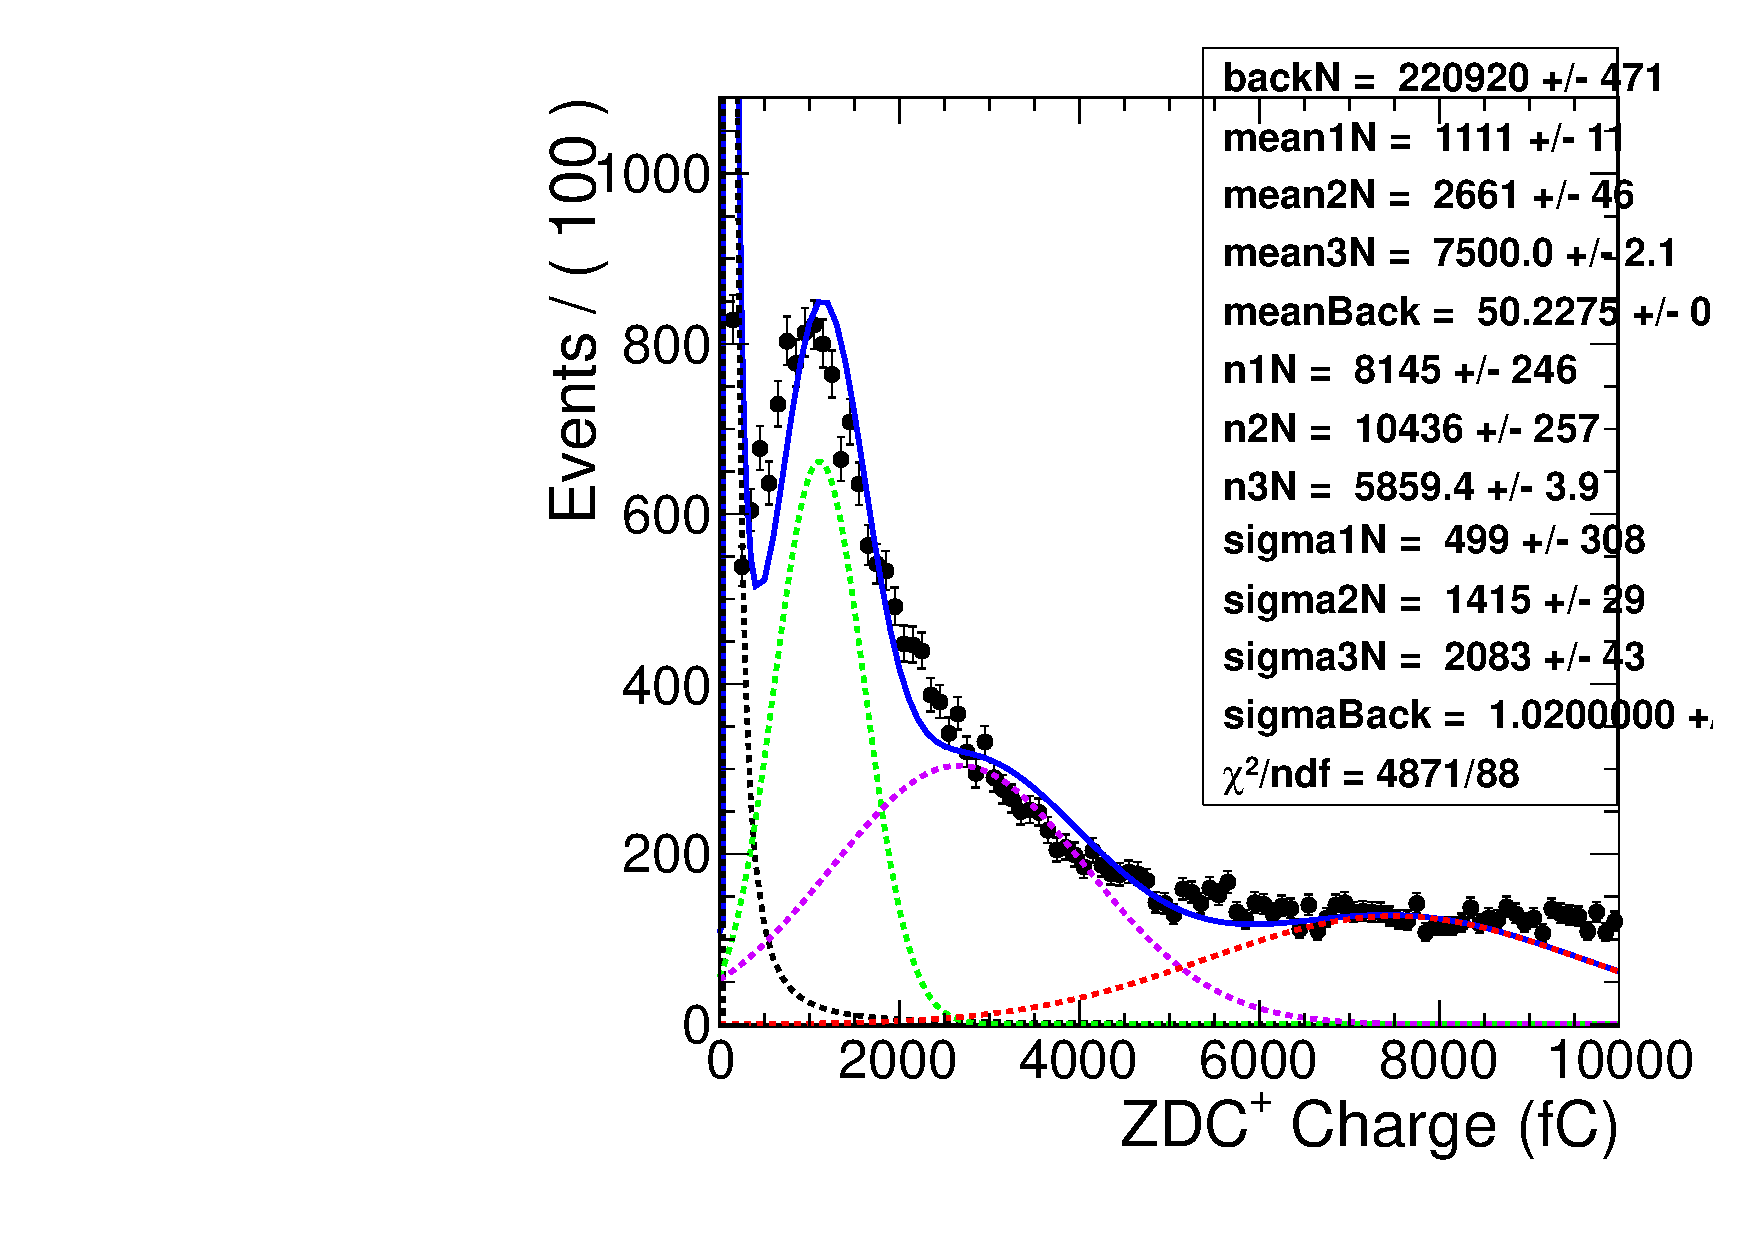
\includegraphics[width=0.45\textwidth]{zdcFit45Pos.pdf}
          \end{array} 
        $
        \caption{Fit to the signal spectra for ZDC$^{-}$ (left) and ZDC$^{+}$ 
          (right)}
        \label{fig:zdcM2Fit}
      \end{figure}
      The threshold for a neutron in the ZDC was taken from the fits in 
        Fig.~\ref{fig:zdcM2Fit}.
      Any signal greater 2$\sigma$ below the mean of the one neutron peak was 
        considered signal.
      Any signal greater than 2$\sigma$ above was considered multiple 
        neutrons.
      The single neutron break up modes were separated from the multiple 
        neutron modes by use of these definitions.

      Several of the break-up mode calculations that have been done involve
        single sided configurations where neutrons are present on one side
        of the interaction point and not the other.
      These modes can be hard to identify because the single neutron peak in 
        ZDC$^{+}$ overlaps with the noise peak at zero.
      To identify events where the ZDCs only measured noise, the noise
        spectra were measured directly.
      Placing an additional criteria based on the ZDCs noise distributions for
        when the ZDCs are devoid of signal provides assurance that the events 
        tagged as single sided events are truly single sided.

      
      The noise distributions for the EM sections and the HAD sections were
        measured separately from out of time time slices.
      In Fig.~\ref{fig:zdcPulseShape} higher than average signal can be seen
        in the 0th time slice, which precedes the main signal time slice 
        time slice 4 by 200 ns. 
      This is due to events where activity was present in the ZDC for 
        two consecutive collisions.
      Time slices 1 and 2, however, occurred between collisions.
      These time slices, which occur out of time, were used to measure the 
        noise spectrum.
      \begin{figure}[!Hhbt]
        \centering
        $ \begin{array}{cc}
          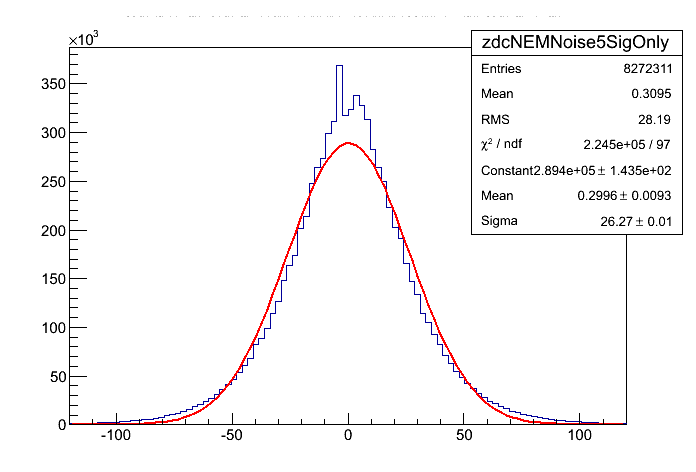
\includegraphics[width=.45\textwidth]{zdcNegEMNoiseFromZBNoCor} & 
          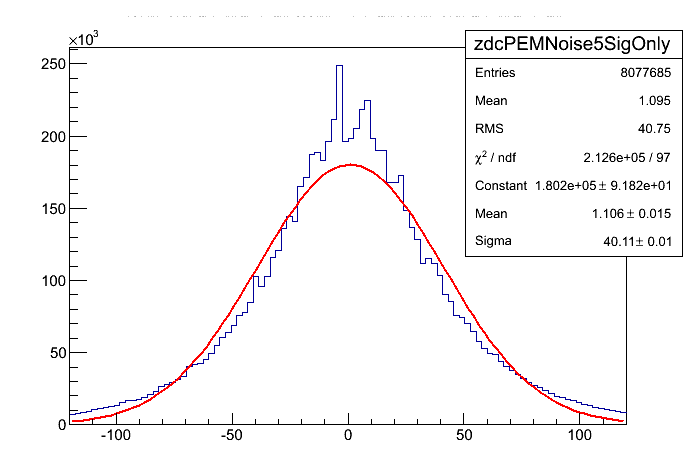
\includegraphics[width=.45\textwidth]{zdcPosEMNoiseFromZBNoCor} \\
          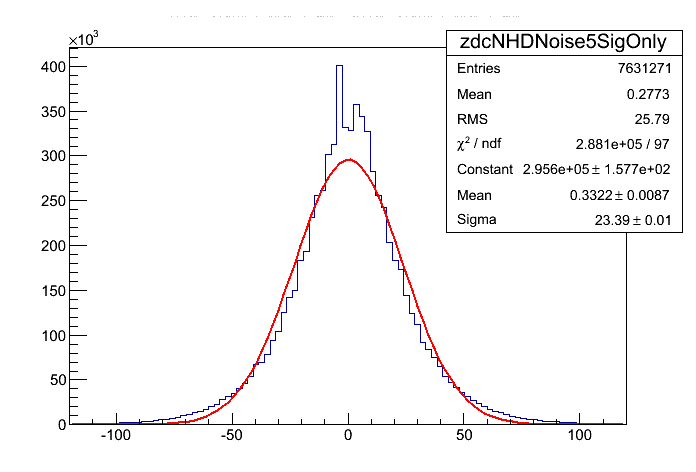
\includegraphics[width=.45\textwidth]{zdcNegHDNoiseFromZB} &
          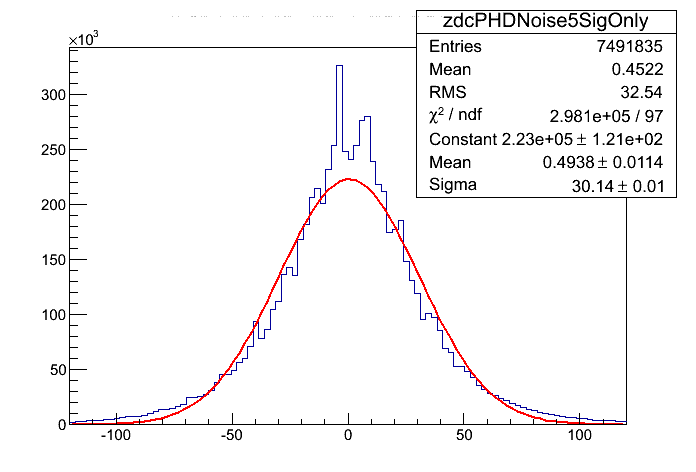
\includegraphics[width=.45\textwidth]{zdcPosHDNoiseFromZB}
        \end{array} $
        \caption{ZDC noise spectra from ZDC$^{-}$ EM section (upper left), 
          ZDC$^{+}$ EM section (upper right), ZDC$^{-}$ HAD section (lower left), 
          and ZDC$^{+}$ HAD section (lower right) from out of time time slices.}
        \label{fig:zdcNoiseSpectra}
      \end{figure}

      As with the signal measurements, the low frequency noise pedestal is 
        subtracted event by event by subtracting time slice 2 from time slice
        1 leaving only the high frequency noise.
      The noise distributions do not depend on the amount of quartz fibers, but
        because the signal does, the noise distributions for EM and HAD sections
        are measured separately.
      Figure~\ref{fig:zdcNoiseSpectra} shows the noise spectrum for each of the 
        EM and HAD sections for the two ZDCs.
      If the HAD or EM signals measured from time slices which match the 
        timing for a collision, time slices 4 and 5, are less than 2$\sigma$ 
        above the mean of the noise distribution or lower, these sections are 
        considered consistent with noise.
      A ZDC is considered consistent with noise if both the HAD section and EM 
        section from that ZDC have signal measurements consistent with noise.

    \subsection{\label{sec:zdcCompare}ZDC reconstruction method comparison}
      In this section the nominal ZDC reconstruction method designed for this
        thesis is compared to an alternative method.
      This additional method, used in previous ZDC measurements, differs 
        in the way the signal time slices are used to calculate the signal from
        each channel.
      In the additional alternative method, the signal is taken from the sum of 
        time slices 4, 5, and 6.
      To estimate the event by event noise pedestal the sum of time slice 
        1 and 2 are used. 
      The signal for an individual ZDC channel is then calculated as the 
        sum of the signal time slices minus the sum of the noise time slices
        weighted by a factor of 3/2 to account for the differing number of 
        noise versus signal time slices.
      As in the nominal method described in Section~\ref{sec:breakUpDet}, 
        the alternative method combines the channels to create a signal 
        measurement from the whole of each side of the ZDC, one
        measurement for ZDC$^{+}$, and one for ZDC$^{-}$.
      The noise subtracted signal from each of the HAD channels are added 
        together.
      Then the EM section channels are summed. 
      The EM section is weighted by a factor of 0.1 as in the nominal method. 
      After the weighting the EM and HAD channels are added to each to create
        one measurement for ZDC$^{+}$ and another measurement for ZDC$^{-}$.
      Figure~\ref{fig:zdcM1Fit} shows the spectra for ZDC$^{+}$ and ZDC${-}$ 
        using the alternative method. 
      The same fit used for the nominal method is applied to the alternative 
        method. 
      As in the nominal method, the single neutron threshold is set to 2$\sigma$
        below the mean from the fit to the one neutron peak.
      The multi-neutron threshold was set to 2$\sigma$ above the one neutron
        peak.
      \begin{figure}[!Hhtb]
        \centering
        $ \begin{array}{cc}
          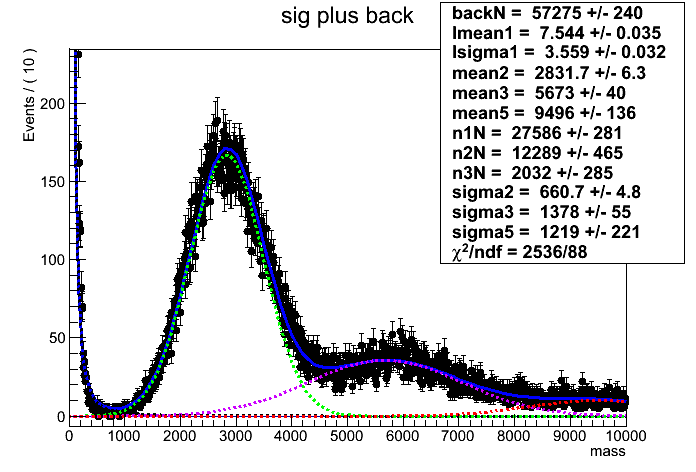
\includegraphics[width=0.45\textwidth]{zdcMinusZBFitTimeCut} &
          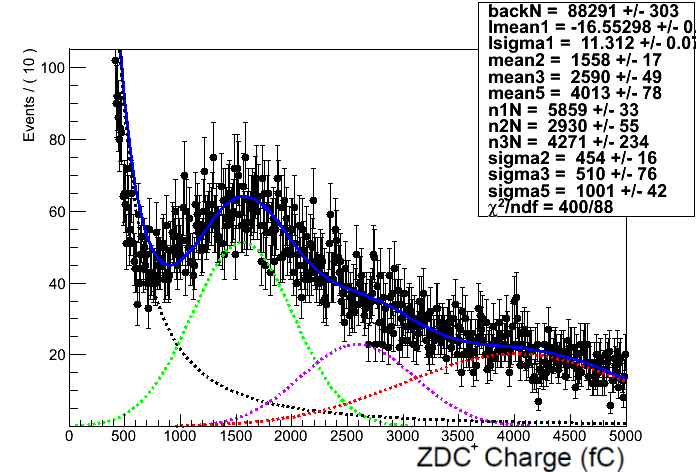
\includegraphics[width=0.45\textwidth]{zdcPlusZBFitTimeCut}
        \end{array} $
        \caption{Fit to charge spectrum from ZDC$^{-}$ (left) and ZDC$^{+}$ 
          (right) using the alternative reconstruction method}
        \label{fig:zdcM1Fit}
      \end{figure}

      The advantage of the alternative method is that by using multiple signal
        and noise time slices the signal and noise are effectively averaged
        reducing time slice to time slice fluctuations.
      However, by using time slices 1 and 2 for measuring the noise, the noise
        can only be measured half the time due to unmeasurable negative 
        fluctuations of the dominant low frequency component of the noise.
      The nominal method relative to the alternative method separates low signal
        from the noise more effectively  for both sides of the ZDC.
      This is particularly important for ZDC$^{+}$ where the 1st HAD section
        had a lower gain than the other sections. 
      The ZDC$^{+}$ and ZDC$^{-}$ signals near the one neutron peak using the
        alternative and nominal reconstruction methods were plotted for comparison in 
        Fig.~\ref{fig:zdcSpec2v1}.
      \DIFdelbegin %DIFDELCMD < \begin{figure}[h]
%DIFDELCMD <         %%%
\DIFdelendFL \DIFaddbeginFL \begin{figure*}[!Hhbt]
        \DIFaddendFL \centering
        \DIFdelbeginFL %DIFDELCMD < 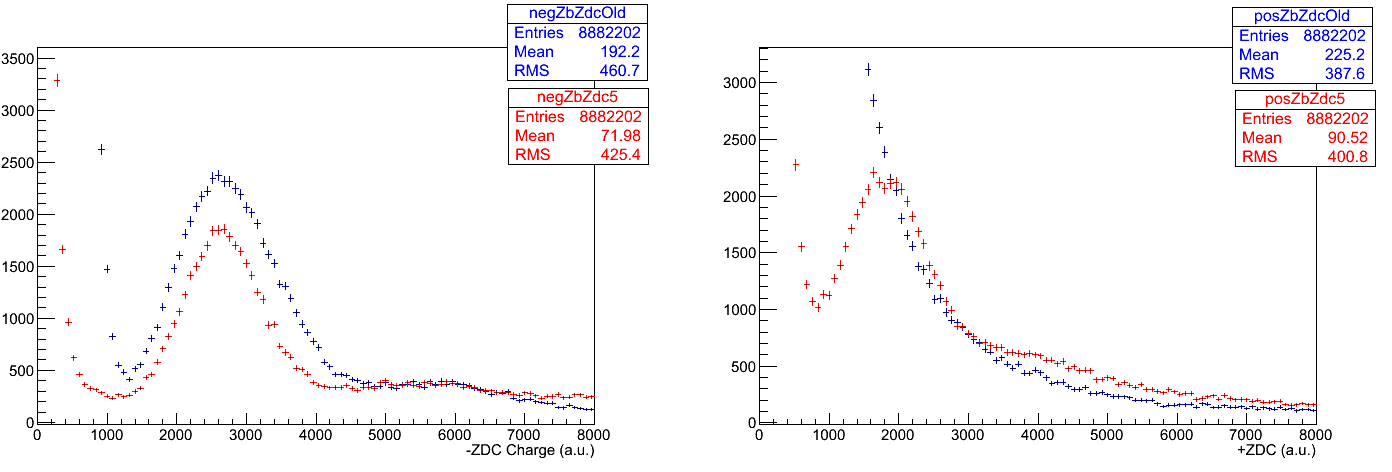
\includegraphics[width=\textwidth]{zdcSpec2v1}
%DIFDELCMD <         %%%
\DIFdelendFL \DIFaddbeginFL 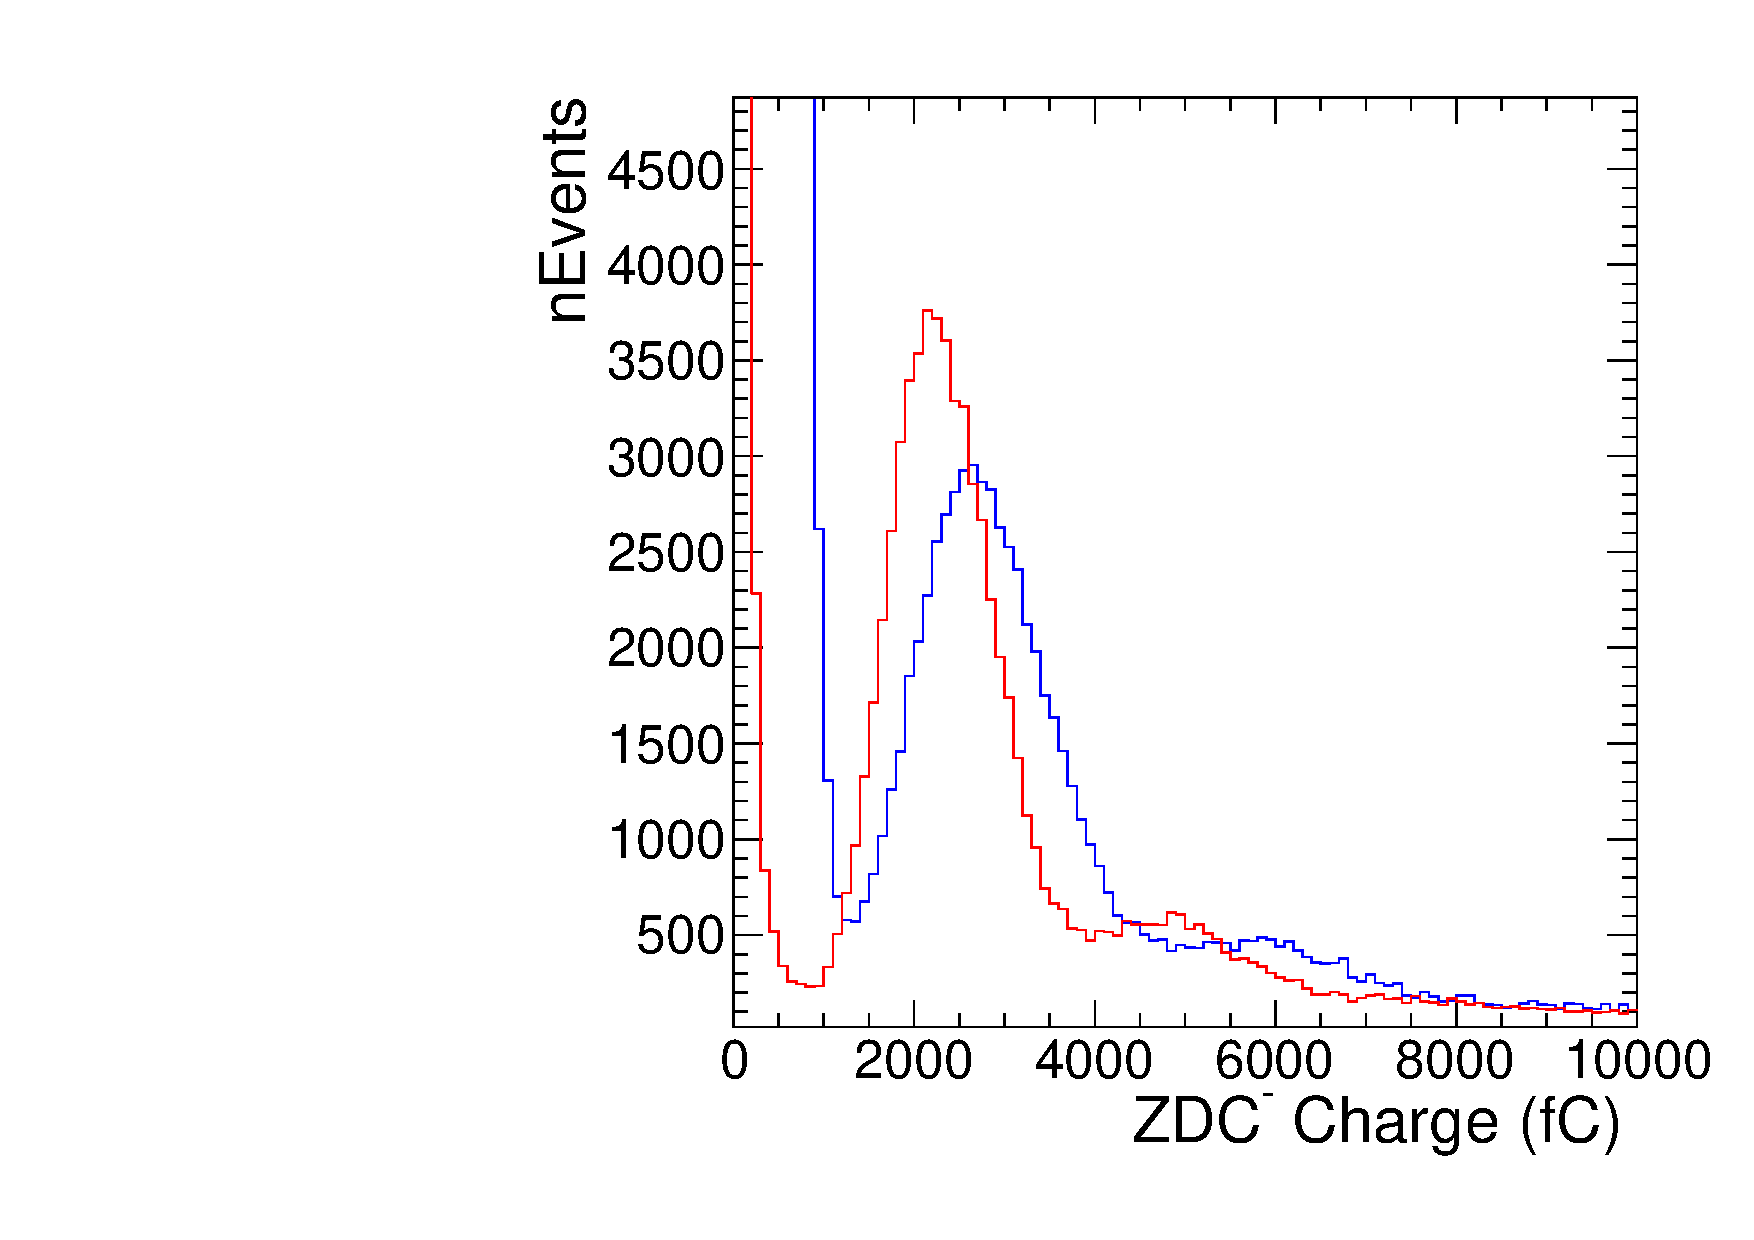
\includegraphics[width=.45\textwidth]{zdcSpec2v1Minus}
        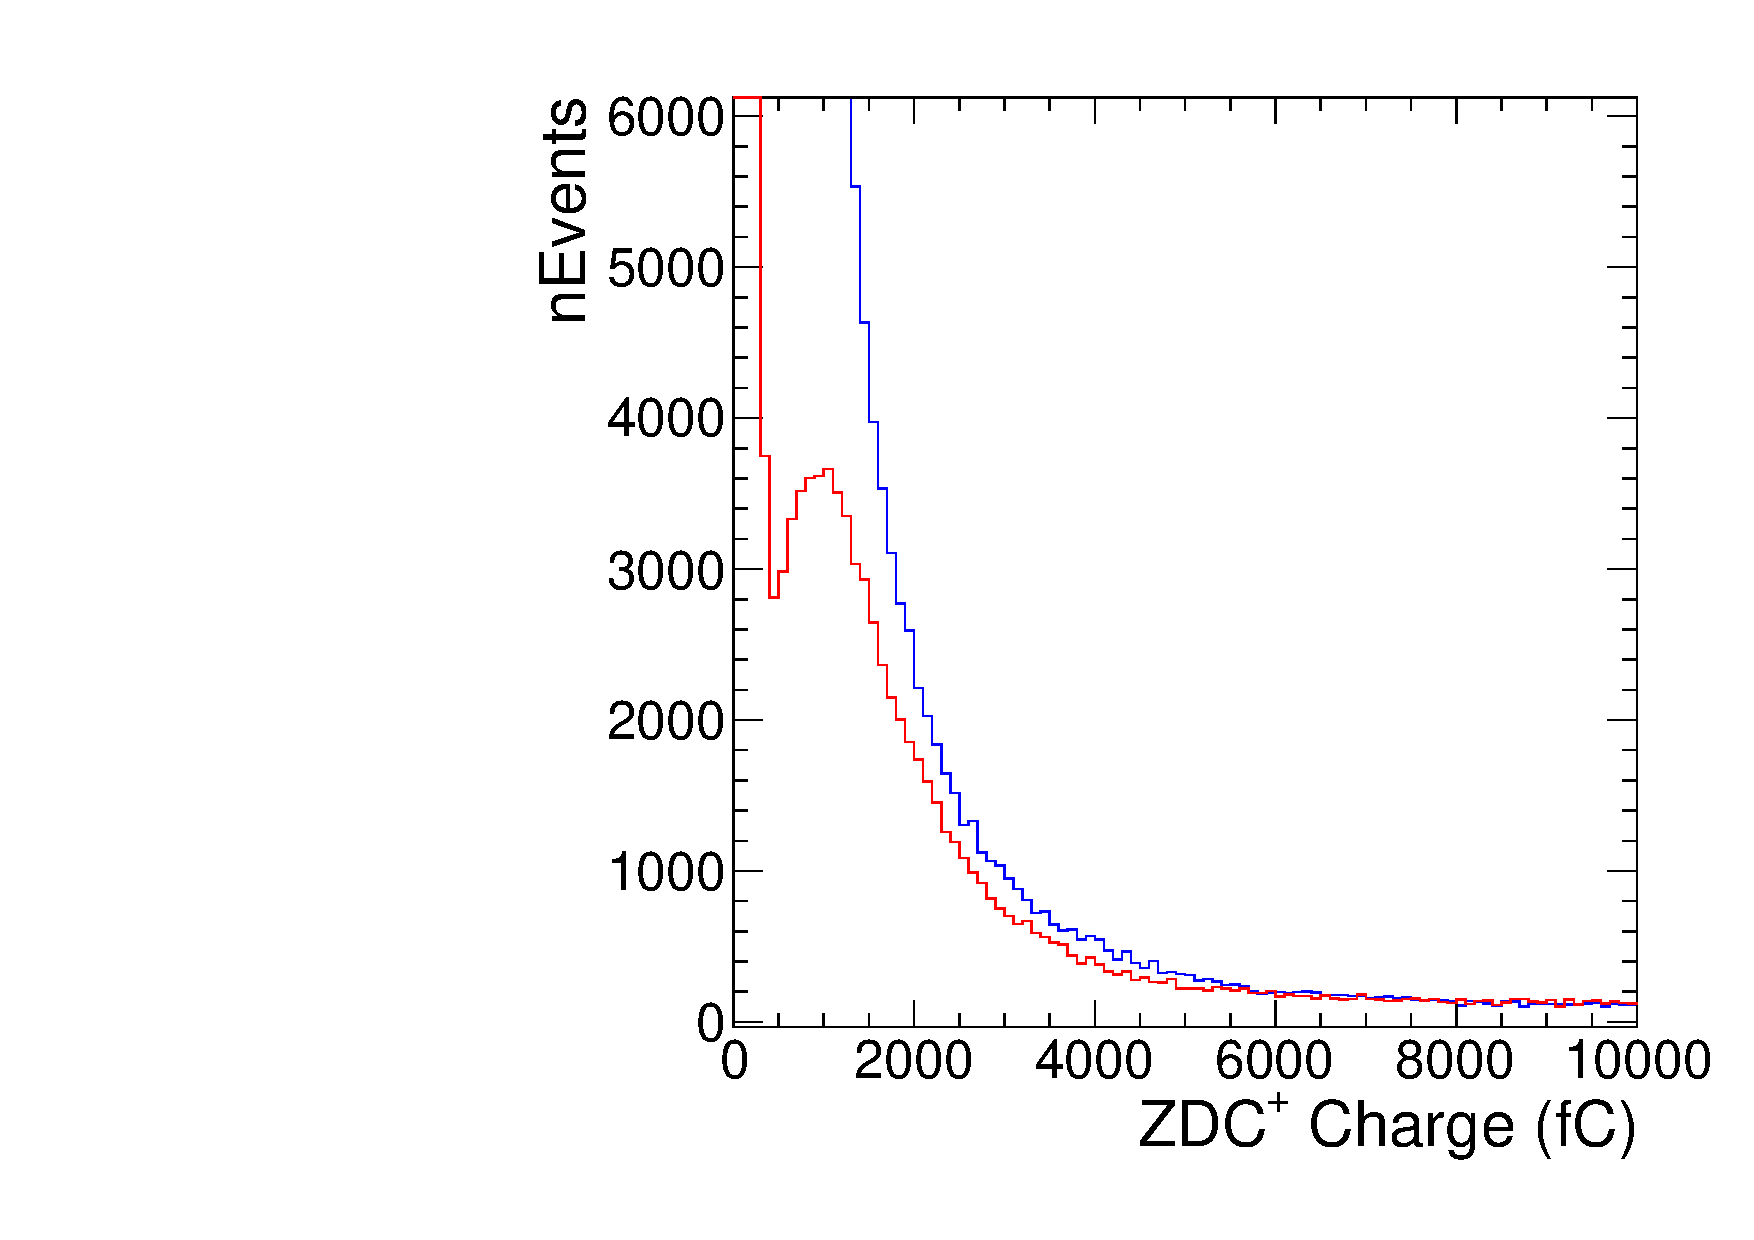
\includegraphics[width=.45\textwidth]{zdcSpec2v1Plus}
        \DIFaddendFL \caption{Comparison of the nominal (red) ZDC reconstruction 
          method and the alternative (blue) method for ZDC$^{-}$ (left) and 
          ZDC$^{+}$ (right).}
        \label{fig:zdcSpec2v1}
      \DIFdelbeginFL %DIFDELCMD < \end{figure}
%DIFDELCMD <       %%%
\DIFdelend \DIFaddbegin \end{figure*}
      \DIFaddend In Fig.~\ref{fig:zdcSpec2v1}, the shrinking of width of the noise peak 
        around zero in the nominal method versus the old method is apparent for
        both ZDC$^{+}$ and ZDC$^{-}$.
      For the alternative method no single neutron peak is resolved in ZDC$^{+}$,
        whereas the single neutron peak is resolved using the nominal method. 

      Timing cuts were applied to enhance the signal relative to the background
        in order to resolve the one neutron peak in ZDC$^{+}$ using the 
        alternative method. 
      Because the products of the collision are synced with time slice 4, noise
        can be rejected by selecting channels where the maximum signal falls 
        into time slice 4.
      The noise will have no preferred time slice (see Fig.~\ref{fig:zdcPulseShape}). 
      Using this fact, neutron events can be selected by requiring that the
        hadronic channels of the ZDC have a peak signal in the fourth time 
        slice.
      Through these timing cuts the single neutron peak was recovered using the
       alternative reconstruction for ZDC$^{+}$.

      To examine the effectiveness of the timing cuts, event by event noise 
        subtraction was removed from the alternative reconstruction.
      The signal from each channel was taken from time slices 4,5, and 6 with
        out subtracting 1 and 2.
      The signal spectrum from ZDC$^{-}$ was then plotted with the result
        shown in Fig.~\ref{fig:zdcTimingCuts}.
      \begin{figure}[!Hhbt]
        \centering
        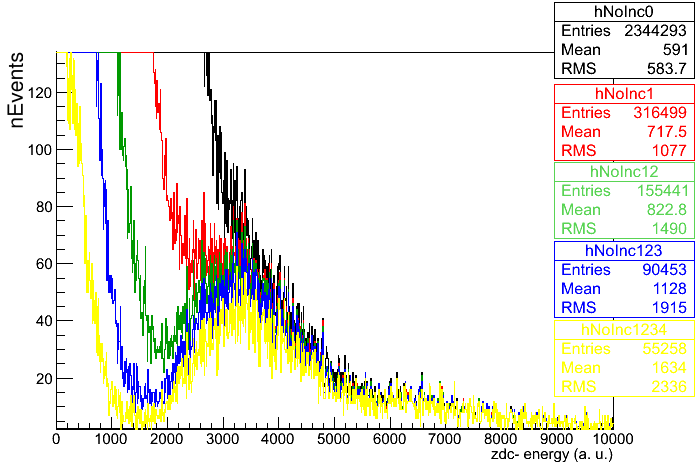
\includegraphics[width=0.6\textwidth]{zdcMinusSingleNuNoInc}
        \caption{Effects of requiring in-time signal in successively more 
          ZDC$^{-}$ hadronic channels, no timing, at least one (red), at least two (green),
            at least three (blue), and all four (yelow) HAD channels have a maximum signal
            in the fourth time slice.}
        \label{fig:zdcTimingCuts}
      \end{figure}
      As each additional hadronic channel is required to have a maximum signal
        in the fourth time slice, the single neutron peak emerges. 
      Figure~\ref{fig:zdcTimingCuts} demonstrates that the single neutron peak 
        can be recovered from the noise using timing cuts alone. 

      Using the alternative noise subtraction method, the same signal that emerges
        from the timing cuts alone appear without timing cuts.
       \begin{figure}[h]
        \centering
        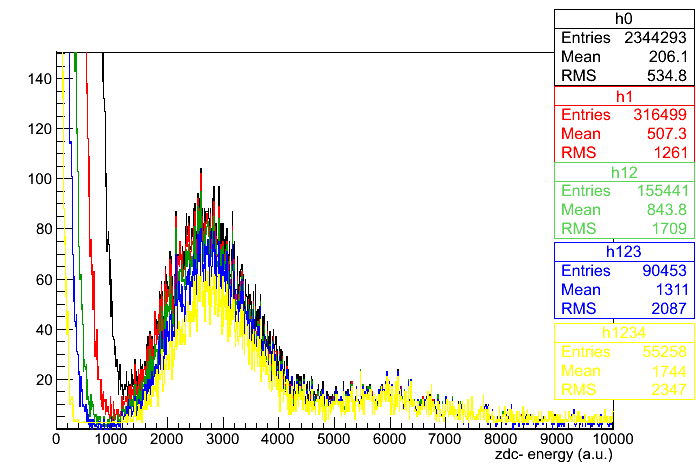
\includegraphics[width=0.6\textwidth]{zdcMinusSingleNuNoSub}
        \caption{Effect of ZDC signal timing requirements after noise 
          subtraction.}
        \label{fig:zdcTimingAfterNoiseSub}
      \end{figure}
      Figure~\ref{fig:zdcTimingAfterNoiseSub} confirms that both noise 
        subtraction and the timing requirement produce the same signal.
      This gives confidence that the signal is not an artifact of either cut, 
        but the true neutron signal.

      Figure~\ref{fig:zdcTimingAfterNoiseSub} and Fig.~\ref{fig:zdcTimingCuts} 
        demonstrate the consistency of using timing cuts and noise 
        subtraction to enhance the signal neutron peak. 
      Figure~\ref{fig:zdcTimingAfterNoiseSub} confirms the legitimacy of the 
        timing requirement method in ZDC$^{-}$ by showing that the same
        signal emerges from the noise subtraction method as the timing method.
      Fig.~\ref{fig:zdcSpec2v1} demonstrates the correspondence between
        the nominal noise subtraction method and the alternative method in 
        ZDC$^{-}$ where the signal is better separated from the electronic noise. 
      This provides confidence that the signal seen in ZDC$^{+}$ using 
        the nominal method is the one neutron peak.

  \chapter{\label{ch:trigg}UPC trigger development for CMS}
  In the 2011 LHC PbPb run the \DIFdelbegin \DIFdel{rate }\DIFdelend \DIFaddbegin \DIFadd{cross section }\DIFaddend of UPC J/$\psi$ production was 
    about 10$^{5}$ times smaller than that of ordinary nucleus-nucleus 
    collisions.
  To recorded these events dedicated UPC triggers were needed. 
  Unlike most heavy-ion triggers, UPC triggers are optimized for low-\pt{} 
    and low multiplicity events. 
  For this reason trigger development specific to UPC events was required to
    carry out the analysis in this thesis.

  The increase in collision rate of the LHC PbPb beams from 2010 to 2011 was
    nearly a factor of 15. 
  To accommodate this increase in rate, the 2011 trigger scheme needed to be 
    more selective than in 2010 where CMS could take any event which 
    appeared to have a collision.
  The available bandwidth was allocated equally amongst the various heavy ion
    analysis groups to pursue as wide a physics program as possible.
  From this consideration, bandwidth limits were placed on the trigger rates
    for each analysis group's trigger package. 

  \section{\label{sec:l1Trigger}L1 trigger}
    The UPC L1 triggers were designed to study UPC \JPsi{} production via the 
      dimuon and dielectron channels (see Section~\ref{sec:detTrg}).
    To achieve this, the loosest muon and electron triggers where combined with
      a trigger on energy in the ZDCs and no activity in BSCs (BSC veto).
    Additional triggers were commissioned in case radiation damage during the 
      run reduced the sensitivity of the BSCs.
    This required no activity in HF (HF veto). 
    These triggers are summarized in Table~\ref{tab:l1Triggers2011}.
    The ECAL2 and ECAL5 triggers in Table~\ref{tab:l1Triggers2011}
      indicate a 2 and 5 GeV threshold on $E_{T}$ measured in the ECAL.
    The MuonOpen trigger indicates that the trigger only 
      requires a muon candidate in one of the three muon sub-systems and that
      there is no momentum threshold.
    ZDC in the trigger names indicate energy constant with at least one neutron.
    The sign on the ZDC label indicates which of the two ZDCs is required. 

    \begin{table}[h]
      \centering
      \begin{tabular}{|l|l|l|l|l|}
        \hline L1 trigger name & Rate (Hz) & Prescale & Id & Type \\ \hline \hline
        MuonOpen and (ZDC$^{+}$~or~ZDC$^{-}$) and BSC veto & 2.1 & 1 & 1 & \multirow{3}{*}{Physics} \\  \hhline{----~}
        ECAL2 and (ZDC$^{+}$~or~ZDC$^{-}$) and BSC veto & 1.8 & 2 & 2 & \\  \hhline{----~}
        ECAL5 and (ZDC$^{+}$~or~ZDC$^{-}$) and BSC veto & 0.3 & 1 & 3 & \\  \hline
        (ZDC$^{+}$~or~ZDC$^{-}$) & 35 & 1500 & 4 & Monitor \\  \hline
        MuonOpen and (ZDC$^{+}$~or~ZDC$^{-}$) and HF veto & 0 & off & 5 & \multirow{3}{*}{Backup} \\ \hhline{----~}
        ECAL2 and (ZDC$^{+}$~or~ZDC$^{-}$) and HF veto & 0 & off & 6 & \\  \hhline{----~}
        ECAL5 and (ZDC$^{+}$~or~ZDC$^{-}$) and HF veto & 0 & off & 7 & \\  \hline
      \end{tabular}
      \caption{List of 2011 L1 seeds.}
      \label{tab:l1Triggers2011}
    \end{table}
    The cumulative L1 trigger rate for all the UPC L1 trigger seeds was
      required to be no greater than 200 Hz.
    This requirement came from the need to keep the tracker read-out rate
      low. 
    The trackers baseline voltage can fluctuate due to the high tracker hit 
      multiplicities in PbPb collisions.
    In order to monitor the zero suppression of the tracker, the zero 
      suppression algorithm was executed using the HLT computing farm 
	      rather than in the tracker firmware.

    The (ZDC$^{+}$ or ZDC$^{-}$) was used to estimate the efficiency of the UPC electron and muon triggers. 
    The factor that the rate is reduced by is called the prescale.
    A prescale of 2 for example means that half the triggers were 
      accepted.
    If the prescale is set to 1, then whole trigger rate is accepted. 
    The prescale factors for the triggers were set to balance the competing objectives 
      of rate reduction and increasing the overlap between the monitoring and
      signal triggers.

  \section{\label{sec:hltTrigger}HLT trigger}
    An event must pass the selection criteria of an HLT path in order to be
      recorded. 
    As opposed to the L1 trigger, which has access only to information from
      calorimeters and muon chambers, the HLT has access to all of the CMS 
      sub-detectors including the tracker. 
    Reconstruction of a track in the pixel detector is used by the UPC 
      trigger paths.
    The use of the pixel detector only, as opposed to using the whole tracker 
      including the silicon strip detector, allows for quick track 
      reconstruction saving computing cycles.
    The UPC triggers were required to have at lease one reconstructed pixel 
      track in order to reject backgrounds where no particles were 
      reconstructed by the tracker.
    For the muon trigger in Table~\ref{tab:hltTriggers2011} the rate was 
      reduced by nearly a factor or 4 compared to its L1 seed rate in 
      Table~\ref{tab:l1Triggers2011}.
    \begin{table}[h]
      \centering
      \begin{tabular}{|l|l|l|l|l|l|}
        \hline HLT trigger  & Rate (Hz) & L1 prescale & HLT prescale & L1 seed & Type \\ \hline \hline
        L1UPCMuon and Pixel Track & 0.52 & 1 & 1 & 1 & \multirow{3}{*}{Physics} \\ \hhline{-----~} 
        L1UPCECAL2 and Pixel Track & 1.65 & 2 & 1 & 2 & \\ \hhline{-----~}
        L1UPCECAL5 and Pixel Track & 0.26 & 1 & 1 & 3 & \\ \hline
        L1ZDCOr & 3.6 & 1500 & 11 & 4 & \multirow{2}{*}{Monitor}  \\ \hhline{-----~}
        L1ZDCOr and Pixel Track & 2.8 & 1500 & 1 & 4 & \\ \hline
        L1UPCMuonHFVeto and Pixel Track & 0 & off & off & 5 & \multirow{3}{*}{Backup}   \\ \hhline{-----~}
        L1UPCECAL2HFVeto and Pixel Track & 0 & off & off & 6 & \\ \hhline{-----~}
        L1UPCECAL5HFVeto and Pixel Track & 0 & off & off & 7 & \\ \hline 
      \end{tabular}
      \caption{List of 2011 HLT trigger.}
      \label{tab:hltTriggers2011}
    \end{table}

    The total HLT output for the UPC trigger package was limited to 20 Hz. 
    The limiting factor for the HLT rate was the amount of disk space given 
      to this analysis. 
    To meet the bandwidth requirements and collect a significant sample
      of data for estimating efficiencies, the prescales were balanced with 
      the goal of achieving at least 5\% statistical precision on the 
      efficiency measurements. 
    As an example of the balancing of the prescales, the HLT  ZDC trigger that 
      did not require a pixel track was given a additional prescale factor 
      of 11 on the HLT.
    The ZDC path that also required a pixel track on the HLT, which used 
      the same L1 seed, was only prescaled at the L1.
    The prescale of 11 was set to ensure that at least 1000 of the pixel track 
      ZDC triggers overlapped with the ZDC L1 only triggers so that efficiency
      of the pixel track requirement in the trigger could be estimated from 
      the tracks lost.

  \section{Studies of 2011 PbPb data}
    The UPC triggers for the 2011 PbPb run make several studies possible.
    Three such studies are discussed below: $\gamma\gamma \rightarrow e^{+} 
      e^{-}$, UPC interactions in peripheral nuclear collisions, and forward
      UPC \JPsi{} using HF. 

    \subsection{High mass $\gamma\gamma \rightarrow e^{+} e^{-}$  in PbPb 2011}
      This measurement would make use of the electron triggers and combine the 
        current dimuon data with dielectron data from the ECAL triggers.
      Because of the smaller mass of the electron,
        dielectron production is slightly favored compared to dimuon 
        production.
      STARlight predicts that dielectron cross section is a factor of 
        2.5 higher in Xn break-up mode than for the dimuons channel when looking 
        at masses above 4 GeV.
      The ECAL is positioned just beyond the tracker, whereas the muon system is 
        the outermost sub-detector.
      Electrons would therefore be less effected by the material budget, which
        is the main factor in reducing yields of reconstructed dimuon 
        candidates.

      The contribution from higher order diagrams can be explored by studying 
        photoproduction of dilepton pairs.
      Because the Pb nucleus has a charge 82 times higher than that of the 
        proton, the electromagnetic coupling is stronger. 
      Thus higher order terms in the perturbative expansion could potentially 
        be more important for the Pb nucleus compared to the proton.
      Recent results by ALICE favor very small contributions for higher order
        terms \cite{Abbas:2013oua}.
      In addition, this analysis provides a useful cross check to the UPC 
        quarkonia analyses such as \JPsi{} by verifying the cross section 
        normalization.

    \subsection{UPC hadronic overlap}
      In the model calculations for UPC quarkonia 
        photoproduction all hadronic interactions are rejected.
      However, inclusive \pt{} spectra of \JPsi{} measured by ALICE in 
        peripheral PbPb collisions show a low momentum peak consistent with 
        coherent photoproduction ~\cite{aliceIclJpsi}.
      \begin{figure}[h]
        \centering
        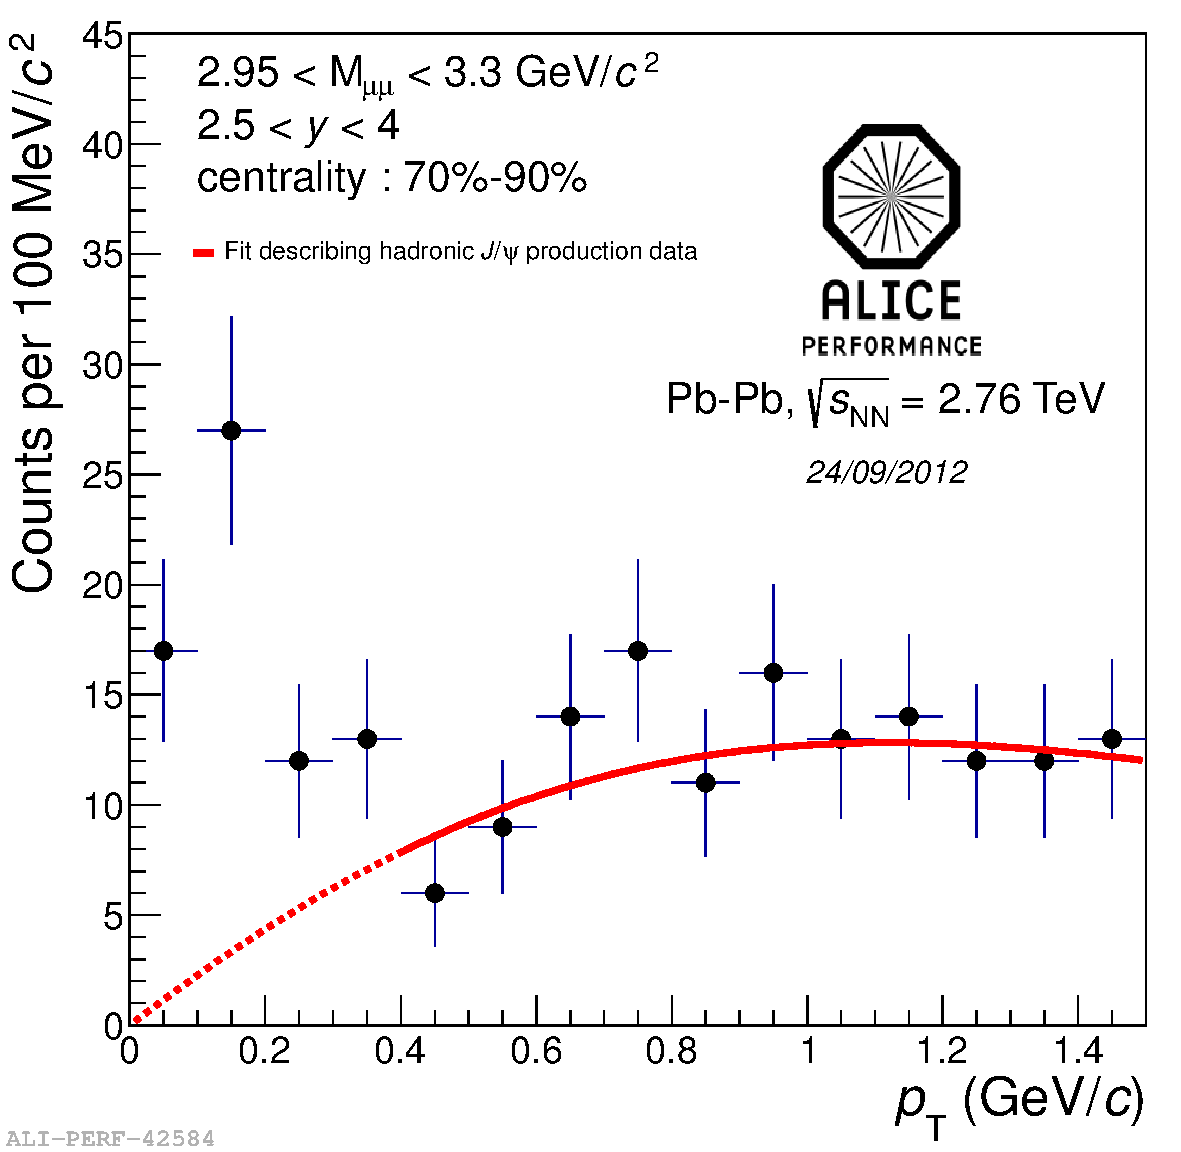
\includegraphics[width=0.5\textwidth]{2012-Sep-24-excess7090.pdf}
        \caption{Coherent excess in inclusive $J/\psi$ $p_{T}$ spectrum.}
        \label{fig:alicePtSpecLowPt}
      \end{figure}
      The ALICE spectra provide hints that UPC processes might also be present 
        in peripheral nucleus-nucleus collisions at the LHC.

      To study the overlap between photoproduction and hadronic production of 
        quarkonium events, the inelastic sample and the UPC sample could both be
        used. 
      The looseness of the rejection criteria to reject hadronic interactions,
        which uses the BSC detectors, leaves a significant overlap with 
        peripheral hadronic collisions. 
      The inclusive quarkonia sample from typical hadronic collisions can also 
        be utilized. 
      Coherent quarkonia photoproduction has a distinctive low $p_{T}$ structure
        that can be used to identify photoproduced candidates in a sample that 
        contains photoproduction combined with hadronic interactions.
      This measurement would open up the door to exploring the boundary between
        photoproduction and hadronic production.

    \subsection{UPC \JPsi{} with electrons in HF}
      As higher rapidities are explored both lower and higher momentum partons
        of the nucleus are probed. 
      Because these two contributions to the UPC photoproduction cross section 
        can be separated using neutron tagging in incoherent events, exploring
        higher dilepton rapidities becomes attractive.
      HF extends to 5 in $\eta$, which is 2.6 units beyond the edge of the 
        tracker.
      By combining hits in HF with tracks in the tracker,  
        \JPsi{} from higher rapidities can be measured. 
      When combined with neutron tagging of incoherently produced quarkonia,
        the current study can be extended to probe lower-$x$ nuclear partons 
        by identifying leptons in HF. 

 \section{\label{sec:pPbTrigDev}Trigger development for the LHC pPb Run}
   Specific UPC triggers were also developed for the pPb run in 2013. 
    For this period of running a much higher total trigger rate was read out 
      relative to 2011.
    The total rate allocated for UPC triggers at the L1 in 2013 was 5 kHz and 
      50 Hz at the HLT.
    This factor of 5 increase in HLT and factor of 25 in L1 bandwidth,
      allowed for a change in emphasis from the L1 to the HLT. 

    The basic strategy in 2013 was the same as in 2012, use the loosest 
      available ECAL and muon L1 triggers to capture the lowest \pt{}
      electrons and muons possible and reject hadronic interactions.
    Because of the L1 bandwidth restrictions in 2011, both the ZDCs and the 
      BCSs were used on the L1 to reduce rates.
    In 2013 only the muon and ECAL triggers were used on the L1 allowing for 
      rejection of hadronic interactions through cuts on track multiplicity. 
    In addition, a more sophisticated trigger using full dimuon reconstructed 
      was developed to increase purity.
    The main advantage in this shift in strategy was a higher purity due to 
      the increased sophistication of the reconstruction on the HLT.
    In addition, the cross section for photoproduciton without regard to 
      neutron emission is higher.
    Therefore, relaxing the requirement of activity in the ZDCs further 
      increases measurable yields. 

    The HLT triggers in 2013 rejected hadronic interactions through counting
      tracks. 
    For the five UPC trigger paths included in the HLT menu, 
      three levels of reconstruction were done at the HLT.

    \begin{itemize}
      \item Pixel tracks were reconstructed from the inner pixel section of the 
        silicon tracker alone, tracks were reconstructed using the full
        tracker using the strips as well, and full dimuon reconstruction was 
        done using the tracker and muon detector. 
      \item The least restrictive pixel track paths required at least 
        one track reconstructed from the pixel detector and less than 10 pixel 
        tracks in the event.
      \item Full tracking paths were added on top of the pixel track paths and included
        an additional requirement of one full track and less than 7 reconstructed
        tracks.
      \item The most restrictive path added to the pixel and full tracking paths and 
        required reconstruction of dimuons with a mass between 2 and 12 GeV.
    \end{itemize}

    \subsection{$J/\psi$ photoproduction in ultra-peripheral pPb collisions}
      The CMS UPC triggers commissioned for the 2013 LHC pPb run will allow for
        further analysis of \JPsi{} photoproduciton.
      In ultra-peripheral pPb collisions, \JPsi{} photoproduciton is dominated 
        $\gamma-p$ interactions~\cite{Frankfurt:2006tp,Guzey:2013taa}.
      The measurement would primarily probe the proton gluon densities.
      In Eq.~\ref{eq:photonFluxFinaltmp} the photon flux depends on the square
        of the number of protons in the parent nucleus, $Z^{2}$. 
      However, the cross section of the target increase as the total 
        number of nucleons to the two thirds power, $A^{2/3}$.
      The much higher photon flux from the Pb-ion compensates for 
        the decreased size of the proton.

      A pPb UPC \JPsi{} measurement will complement the measurements done at 
        HERA~\cite{Chekanov:2002xi,Aktas:2005xu,Alexa:2013xxa}, and measurements done by ALICE~\cite{TheALICE:2014dwa}.
      CMS will contribute by adding additional kinematic coverage and cover a 
        unique range of $\gamma$p center of mass energies, $W_{\gamma p}$. 
      The difference in beam energies and species at LHC versus HERA result in
        access to different $W_{\gamma p}$. 
      ALICE and CMS have different acceptance in \JPsi{} rapidity, which also 
        translates to coverage of different $W_{\gamma p}$.
      In addition, an excess in the UPC cross section compared to HERA 
        measurements would indicate a non-exclusive contribution to the pPb UPC 
        \JPsi{} cross section. 
      This measurement will enhance the current understanding of 
        the \JPsi{} photoproduction cross section as a function of the 
        photon-proton center of mass energy, $W_{\gamma p}$.

  \chapter{Analysis}
  In \DIFdelbegin \DIFdel{the following }\DIFdelend \DIFaddbegin \DIFadd{this }\DIFaddend chapter the various parts of the measurements done for this
    thesis are explained. 
  The following chapter contains seven sections explain each of these parts: 
    \DIFdelbegin \DIFdel{mc }\DIFdelend \DIFaddbegin \DIFadd{Monte Carlo }\DIFaddend simulation, trigger development, data sets and event selection,
    break-up determination, signal extraction, efficiency determination,
    and systematic checks. 
  In Section~\ref{sec:mcSim}\DIFaddbegin \DIFadd{, }\DIFaddend the simulations used to \DIFdelbegin \DIFdel{estimated }\DIFdelend \DIFaddbegin \DIFadd{estimate }\DIFaddend the detectors 
    ability to measure UPC processes \DIFdelbegin \DIFdel{is }\DIFdelend \DIFaddbegin \DIFadd{are }\DIFaddend discussed. 
  Section~\ref{sec:TrigDev} explains the considerations that went into the 
    triggers which were developed for the analyses discussed in this thesis.
  How the final events were selected and how triggers were used to separate the
    data in to data sets is detailed in Section~\ref{sec:DataSetEvSel}.
  Extraction of the number of events from each of the three physics processes 
    discussed in this thesis, coherent, incoherent, and photon-photon process
    from the final selected events is discussed is Section~\ref{sec:sigEx}.
  The \DIFdelbegin \DIFdel{estimates }\DIFdelend \DIFaddbegin \DIFadd{determination }\DIFaddend of the detectors efficiency for measuring UPC events is 
    explained in Section~\ref{sec:effDet}.
  Section~\ref{sec:sysCheck} lays out how the systematic uncertainties are 
    estimated.

  \section{\label{sec:mcSim} MC \DIFdelbegin \DIFdel{Simulation}\DIFdelend \DIFaddbegin \DIFadd{simulation}\DIFaddend }
    Every physical measurement is the product of the underlying physics 
      \DIFdelbegin \DIFdel{convolved }\DIFdelend \DIFaddbegin \DIFadd{folded }\DIFaddend with the response of the detector used to do the measurement. 
    In order to understand the underlying physical process, the detector's 
      effect on the measurement must be understood and accounted for. 
    As instruments become more and more complicated, the interplay between all
      of the many parts of the detector makes an analytic approach to the 
      problem untenable.
    For this reason, the numerical technique of Monte Carlo (MC) simulation is
      the most useful approach.

    MC simulations use random number generation to solve the problem 
      numerically by brute force. 
    First, particles are generated according the theoretical distributions.
    These particles are then propagated through a simulation of the detector.
    As the particles pass through the detector, random numbers are again used
      to determine how these particles interact with the materials of the 
      detector based on the known properties of the material. 
    In this way, the theoretical distributions are merged with the \DIFdelbegin \DIFdel{complicated 
      }\DIFdelend \DIFaddbegin \DIFadd{realistic 
      }\DIFaddend response of the detector. 
    The collective combination of the many sub \DIFdelbegin \DIFdel{detectors }\DIFdelend \DIFaddbegin \DIFadd{detector }\DIFaddend responses with the 
      theoretical distributions emerges from the successive creation of random
      events.
    The result is the convolved response of the detector with the underlying 
      physical process that is to be studied. 

    In this thesis, two main classes of MC simulation samples were used. 
    The first class uses STARlight to generate events.
    This class of MC samples corresponds to the theoretical calculations 
      described in \DIFdelbegin \DIFdel{in }\DIFdelend Section~\ref{sec:vdmTheory}.
    There are three different physical process described.
    Coherent J/$\psi$ production, where the photon couples to the nucleus as
      a whole, incoherent J/$\psi$ production, where the photon couples to a
      nucleon within the nucleus, and \DIFaddbegin \DIFadd{the }\DIFaddend photon-photon process, where the 
      photons from the two nuclei interact with each other to produce a lepton 
      pair directly.
    All three STARlight \DIFdelbegin \DIFdel{sample }\DIFdelend \DIFaddbegin \DIFadd{samples }\DIFaddend produce a $\mu^{+}$ and $\mu^{-}$ in the final 
      state that interacts with the detector.
    The second class uses PYTHIA6 to decay J/$\psi$s with a given
      input $p_{T}$ and rapidity distribution.
    Two samples of this class of particle gun data were produced each with 
      different $p_{T}$ distributions (See Fig.).

    \DIFdelbegin \DIFdel{The software chain used for producing the STARlight samples has five steps.
    }\DIFdelend Because STARlight is not integrated into the standard CMS software 
      framework (CMSSW), \DIFdelbegin \DIFdel{this chain }\DIFdelend \DIFaddbegin \DIFadd{a simulation software chain using STARlight }\DIFaddend was 
      developed for the analysis described in this thesis.
    \DIFaddbegin \DIFadd{The software chain used for producing the STARlight samples has five steps.
    }\DIFaddend First, STARlight is run in the specified mode, and a single file is 
      created for each physics process, for this thesis, one file for the 
      coherent process, the incoherent process, and the photon-photon process
      for a total of three files.
    The output from the STARlight generator is in a format specific to 
      STARlight, therefore, the output from the original generation step is 
      then converted to the Les Houches (LHE) format. 
    In this conversion to LHE format, either the parent J/$\psi$ for the 
      J/$\psi$ production samples, or the initial photon-photon pair are added
      to the LHE output file.
    The standard STARlight output only includes the final state particles.
    Additionally, the initial output from STARlight is split into a collection 
      of smaller LHE files so that each of the smaller samples can be 
      processed in parallel.
    Each of the LHE files is used as input to CMSSW.
    The three remaining steps take place within the \DIFdelbegin \DIFdel{frame work}\DIFdelend \DIFaddbegin \DIFadd{framework}\DIFaddend . 
    First the generated particles are propagated through the GEANT4 detector 
      simulation.
    This accounts for all the interactions with the detector and produces as 
      output a format identical to the raw data that is recorded during data
      taking.
    The next two steps are identical to data taking.
    The reconstruction software used during data taking is run on the output 
      of the detector simulation, and last, the output of the reconstruction
      is reduced to the information that is needed for the final analysis.

    The particle gun samples were created entirely within CMSSW.
    An interface to PYTHIA6 is included within CMSSW, which takes J/$\psi$
      $p_{T}$ and rapidity distributions as input. 
    The J/$\psi$ are created according to the input distributions, and then uses
      PYTHIA6 to decay the J/$\psi$s to $\mu^{+}$ and $\mu^{-}$.
    As with the STARlight samples, these muons are propagated through the GEANT4
      simulation of the detector, and the raw data is produced.
    The remaining steps of running the reconstruction code and reducing the 
      data to the final data needed for the analysis are identical to the 
      STARlight production.

    The five MC samples, three STARlight samples, and two particle gun samples,
      differ primarily in the $p_{T}$ distribution of the J/$\psi$s produced
      and the polarization of the J/$\psi$s, which effects angle at which
      the muon daughters are emitted relative to the direction in which the
      J/$\psi$ is traveling. 
    In Fig.~\ref{fig:starlightRapPtDist} the $p_{T}$ of J/$\psi$s from the 
      coherent and photon-photon samples are peaked steeply a low $p_{T}$, and 
      neither sample extends much beyond 0.15 GeV in $p_{T}$.
    The incoherent sample is peaked near 0.5 GeV and extends beyond 1 GeV.
    The two particle gun samples resemble the incoherent and coherent samples.
    The first sample has a Gaussian $p_{T}$ distribution extending to 
      approximately 0.15 GeV, whereas the second is flat in $p_{T}$ up to
      2 GeV.
    The particle gun samples are unpolarized, whereas the STARlight samples 
      have transverse polarization. 
    \DIFdelbegin \DIFdel{Therefor}\DIFdelend \DIFaddbegin \DIFadd{Therefore}\DIFaddend , the particle gun samples there is no preferred direction for the 
      emission of the daughter muons.
    In the STARlight samples however the daughters tend to be emitted in line
      with the direction of the J/$\psi$'s momentum.
    This is particularly pronounced for the photon-photon process.

    \begin{figure}[!Hhbt]
      \centering
      $ \begin{array}{cc}
        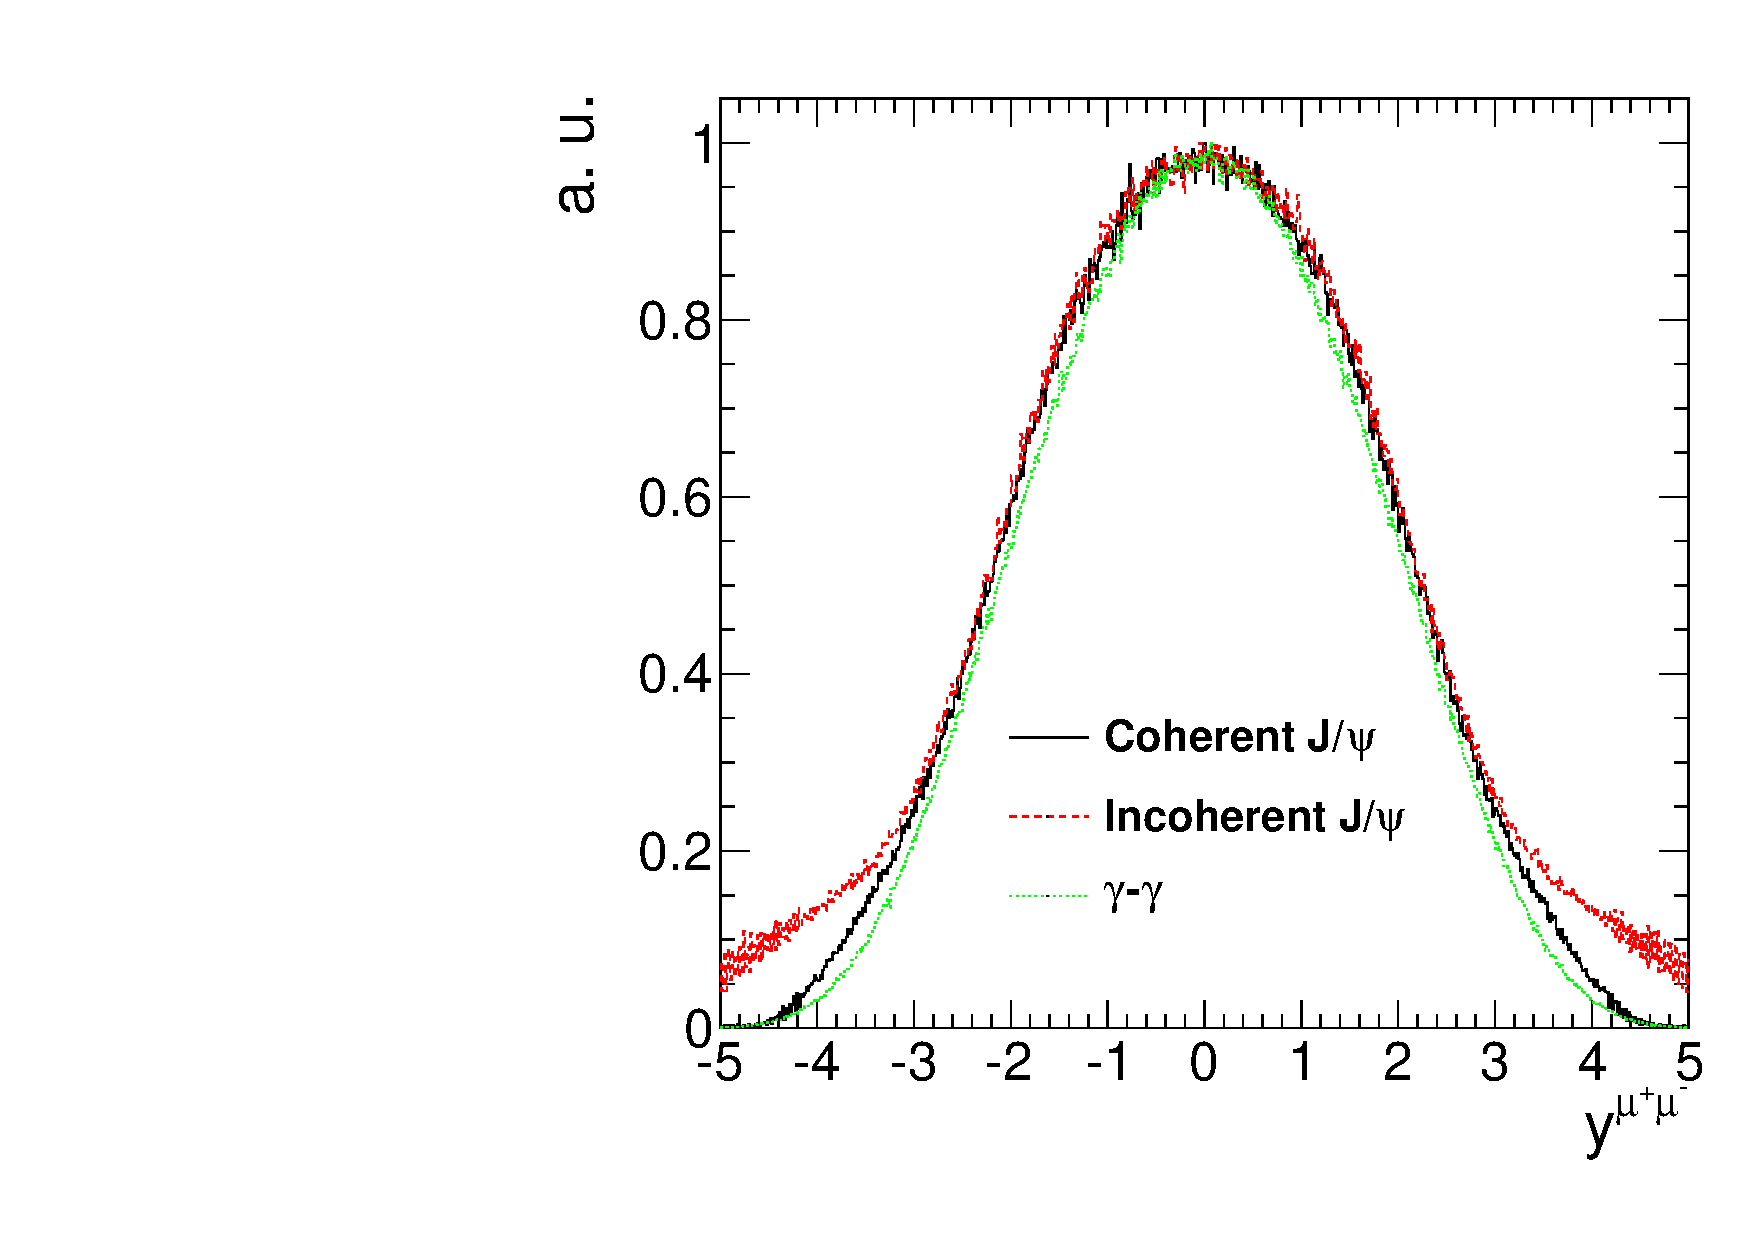
\includegraphics[width=0.45\textwidth]{genRapDis} &
        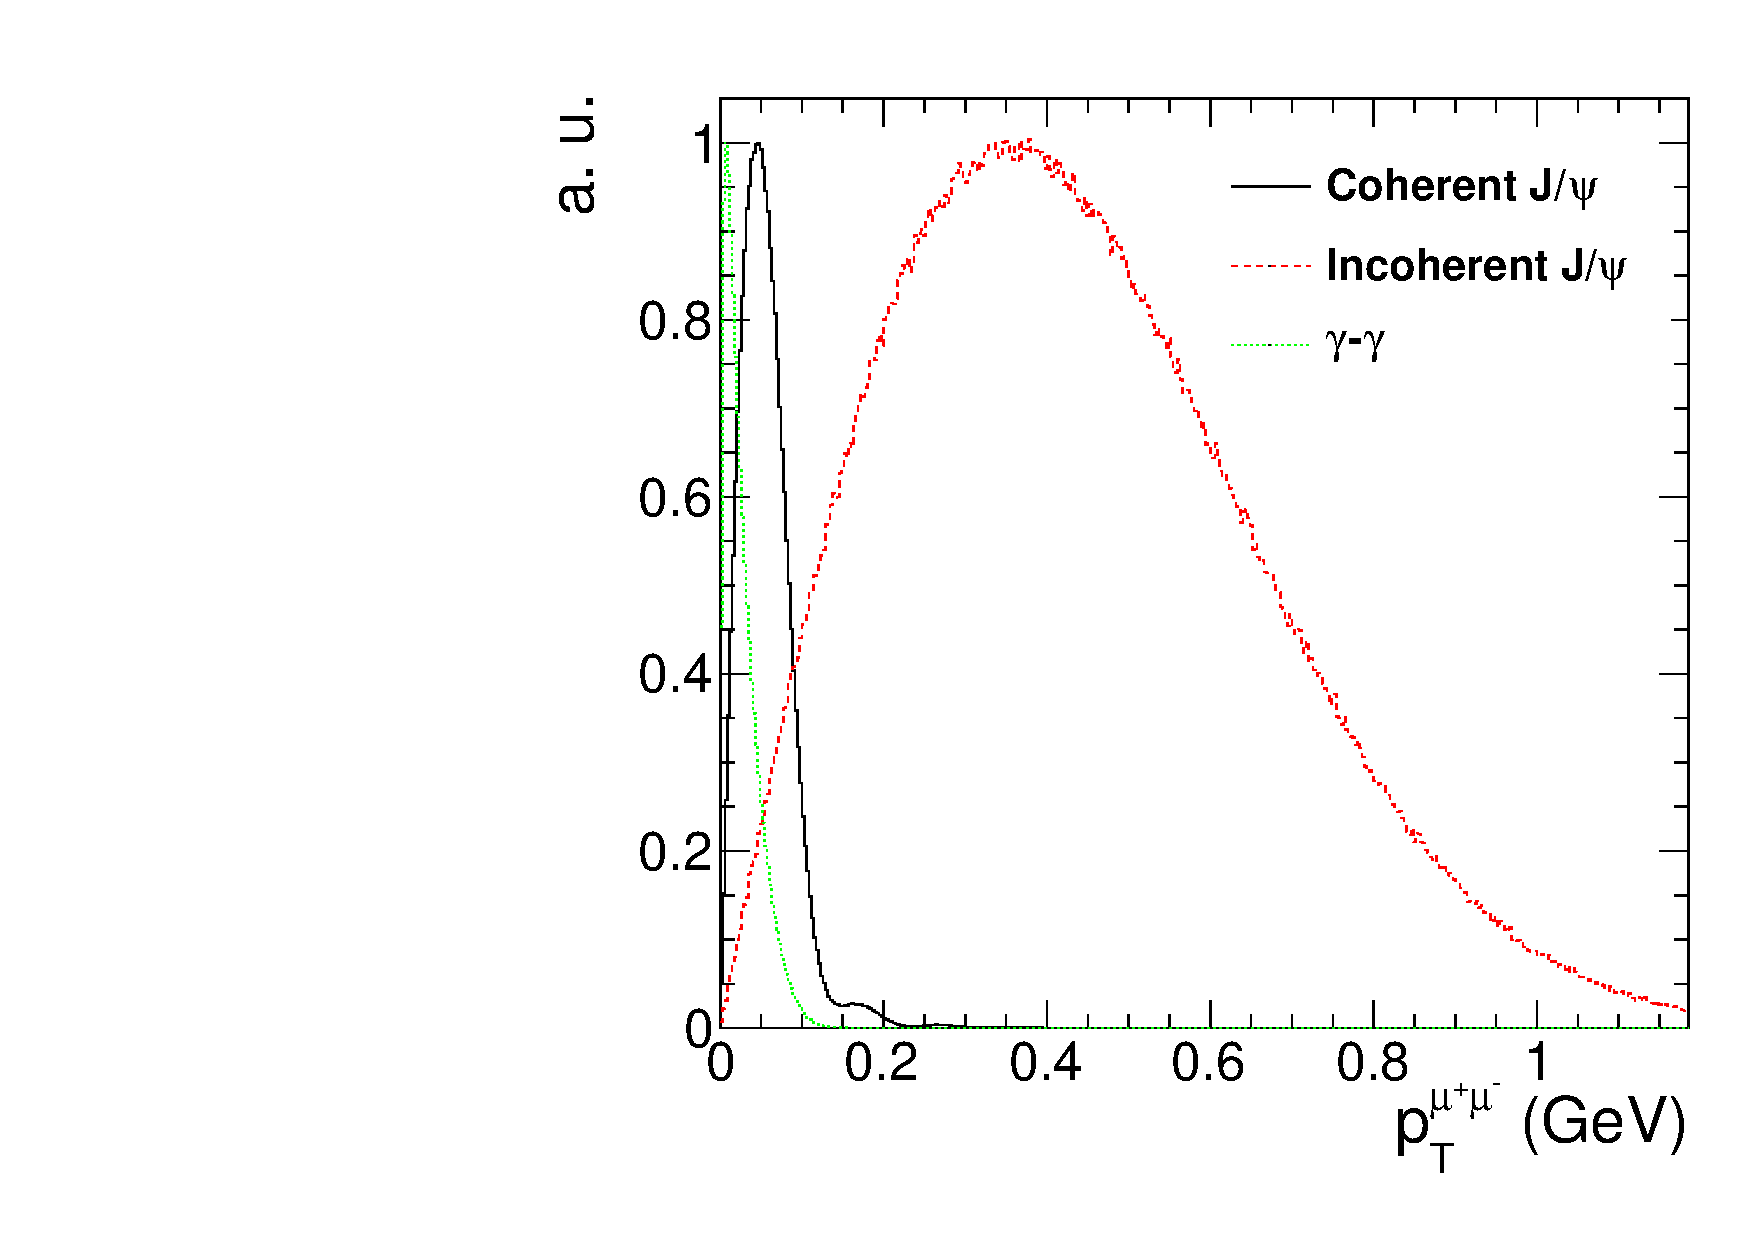
\includegraphics[width=0.45\textwidth]{genPtDis}
      \end{array} $
      \caption{Generator level rapidity (left) and $p_{T}$ (right) 
          distributions for the coherent \DIFaddbeginFL \DIFaddFL{(black)}\DIFaddendFL , \DIFdelbeginFL \DIFdelFL{\textcolor{red}{incoherent}}\DIFdelendFL \DIFaddbeginFL \DIFaddFL{incoherent (red)}\DIFaddendFL , 
          and \DIFdelbeginFL \DIFdelFL{\textcolor{green}{photon-photon} }\DIFdelendFL \DIFaddbeginFL \DIFaddFL{photon-photon }\DIFaddendFL process \DIFaddbeginFL \DIFaddFL{(green).}\DIFaddendFL }
      \label{fig:starlightRapPtDist}
    \end{figure}

    \begin{figure}[!Hhbt]
      \centering
      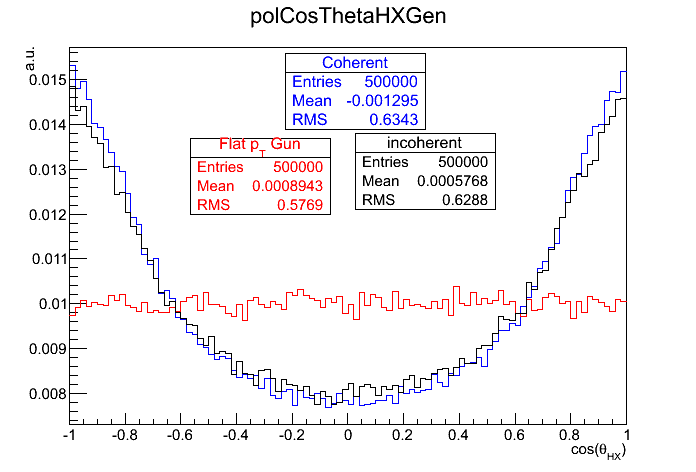
\includegraphics[width=.6\textwidth]{polCosThetaHXGen}
      \caption{ The J/$\psi$ polarization of the \DIFdelbeginFL \DIFdelFL{\textcolor{red}{particle gun}
        }\DIFdelendFL \DIFaddbeginFL \DIFaddFL{particle gun (red)}\DIFaddendFL ,
        \DIFdelbeginFL \DIFdelFL{\textcolor{blue}{coherent}}\DIFdelendFL \DIFaddbeginFL \DIFaddFL{coherent (blue)}\DIFaddendFL , and incoherent samples are plotted as the
        cosine of the helicity angle.} 
      \label{fig:genHXAngle}
    \end{figure}
\DIFdelbegin %DIFDELCMD < 

%DIFDELCMD <     %%%
\DIFdelend %DIF > %%%%Fix this paragraph%%%%%%
    The momentum of the final state muons is the main drivers of whether the 
      candidate can be measured. 
    The polarization and the $p_{T}$ distribution of dimuons from the generator
      determine the momentum of the daughters. 
    The \DIFdelbegin \DIFdel{low $p_{T}$ of the J/$\psi$ restricts the momentum of the $\mu^{+}$ and
      $\mu^{-}$ daughters produced from the J/$\psi$ decay. 
    The }\DIFdelend polarization effects how the momentum is shared between the daughters.
    In the rest frame of the parent particle from which the daughters decay\DIFaddbegin \DIFadd{,
      }\DIFaddend equal momentum is given to each daughter. 
    However in the lab frame of the detector, the muon daughters which are 
      emitted from transversely polarized J/$\psi$ will tend to be emitted in
      the direction of J/$\psi$ and will have unequal momentum in the lab 
      frame.
    The daughter traveling in the direction of the J/$\psi$ will have increased
      momentum, whereas the daughter traveling opposite to the J/$\psi$ 
      direction will have decreased momentum. 
    The combination of these two effects create a muon with very low momentum 
      compared to the typical momenta of muons measured by CMS. 
    The momentum of the lower momentum muon daughters is the main restriction
      on whether or not the J/$\psi$ can be measured. 
%DIF > %%%%Fix this paragraph%%%%%%

  \section{\label{sec:TrigDev} Trigger \DIFdelbegin \DIFdel{Development}\DIFdelend \DIFaddbegin \DIFadd{development}\DIFaddend } 
    \DIFdelbegin \DIFdel{Prior to the }\DIFdelend \DIFaddbegin \DIFadd{CMS collected dedicated UPC triggers for the first time during the }\DIFaddend 2011 
      \DIFdelbegin \DIFdel{LHC PbPb run, UPC events had not been directly studied in 
      PbPb collisions using CMS}\DIFdelend \DIFaddbegin \DIFadd{PbPb run}\DIFaddend .
    Design of the UPC triggers required studies of the 2010 data to estimate 
      rates and \DIFdelbegin \DIFdel{insure }\DIFdelend \DIFaddbegin \DIFadd{ensure }\DIFaddend that the bandwidth used by these trigger would be
      sufficiently low. 
    All the different physics analyses must share the limited readout rate of 
      the detector.
    For this reason, conservation of bandwidth was a major design consideration.

    \DIFdelbegin \DIFdel{To estimate the 2011 rates prior to the run, the }\DIFdelend \DIFaddbegin \DIFadd{The }\DIFaddend 2010 rates were used to extrapolate to the interaction rate of the 2011 \DIFaddbegin \DIFadd{i
      }\DIFaddend run. 
    The unique UPC triggers were estimated by combining existing triggers from
      the 2010 run. 
    By calculating the ratio between the UPC trigger rates and the minimum bias
      trigger rate, the UPC trigger rates were scaled up to the 2011 
      interaction rates using the 2010 data. 
    The extrapolated rates allowed for a package triggers to be created that 
      fit within the bandwidth requirement of CMS Heavy Ions group. 

    The trigger package for 2011 contained ZDC based efficiency monitoring 
      triggers, muon and electron based triggers for measuring J/$\psi$, and 
      backup triggers in case there was a problem with the original muon and 
      electron triggers.
    In order to \DIFdelbegin \DIFdel{recorded }\DIFdelend \DIFaddbegin \DIFadd{record }\DIFaddend the trigger efficiency monitoring data, the ZDC 
      triggers had to be prescaled to a lower rate. 
    The scaling down of the monitoring triggers were setup to insure overlap
      with the signal triggers.
    By balancing the competing objectives of rate reduction and increasing 
      the overlap between the monitoring and signal triggers, 
      the prescales for the trigger were as seen in Table\DIFdelbegin \DIFdel{.%DIF < ~\ref{triggerTabel2011}.
}\DIFdelend \DIFaddbegin \DIFadd{~\ref{triggerTabel2011}.
}\DIFaddend 

    \subsection{\label{sec:l1Trigger} L1 \DIFdelbegin \DIFdel{Trigger}\DIFdelend \DIFaddbegin \DIFadd{trigger}\DIFaddend }
      The goal of the L1 triggers was to record enough data to measure dimuons
        and dielectrons in UPC events.
      To achieve this, the loosest muon trigger and lowest threshold ECAL 
        triggers where paired with a trigger on energy in the ZDC and a veto on
	      energy in the BSC.
      Additional triggers \DIFdelbegin \DIFdel{which }\DIFdelend \DIFaddbegin \DIFadd{that }\DIFaddend vetoed on energy in HF were commissioned in case
        radiation \DIFdelbegin \DIFdel{damaged to the }\DIFdelend \DIFaddbegin \DIFadd{damage during the run reduced the sensitivity of }\DIFaddend BSCs.
      The L1 package that was constructed for the analysis of UPC J/$\psi$ 
        is presented in Table~\ref{tab:l1Triggers2011}.

%DIF > %%%%%Fix this table%%%%%%%%%%%%%%%%%%%%%%%%%%
      \begin{table}[h]
        \centering
        \begin{tabular}{|l|l|}
          L1 Trigger Seed  & Type \\ \hline \hline
          L1\_MuOpen\_ZdcCalo\_NotBscMinBiasThresh2\_BptxAND & Physics \\  \hline
          L1\_EG2\_ZdcCalo\_NotBscMinBiasThresh2\_BptxAND & Physics \\  \hline
          L1\_EG5\_ZdcCalo\_NotBscMinBiasThresh2\_BptxAND & Physics \\ \hline
          L1\_ZdcCaloMinus\_BptxAND & Monitor \\  \hline
          L1\_ZdcCaloMinus\_BptxAND & Monitor \\  \hline
          L1\_MuOpen\_ZdcCalo\_NotHcalHfCoincidencePm\_BptxAND & Backup \\ \hline
          L1\_EG2\_ZdcCalo\_NotHcalHfCoincidencePm\_BptxAND & Backup \\ \hline
          L1\_EG5\_ZdcCalo\_NotHcalHfCoincidencePm\_BptxAND & Backup \\ \hline \hline
        \end{tabular}
        \caption{List of 2011 L1 seeds.}
        \label{tab:l1Triggers2011}
      \end{table}
\DIFdelbegin %DIFDELCMD < 

%DIFDELCMD <       %%%
\DIFdelend %DIF > %%%%%Fix this table%%%%%%%%%%%%%%%%%%%%%%%%%%
      The cumulative L1 trigger rate for all the UPC L1 trigger seeds was
        required to be 200 Hz.
      This requirement stemmed from the need to keep the tracker read-out rate
        low. 
      The trackers baseline voltage can fluctuate due to the high tracker hit 
        multiplicities in PbPb collisions.
      In order to monitor the zero suppression of the tracker, the zero 
        suppression algorithm was executed using the HLT computing farm 
	      rather than \DIFdelbegin \DIFdel{the }\DIFdelend in the tracker firmware.
      The rate at which the tracker could be readout without zero suppression
        set the limit for the L1 bandwidth.


    \subsection{HLT \DIFdelbegin \DIFdel{Trigger}\DIFdelend \DIFaddbegin \DIFadd{trigger}\DIFaddend }
      As opposed to the L1 trigger, which reads out the tracker, the HLT has 
        access to the tracker information. 
      Reconstruction of a track in the pixel detector is used by the UPC paths.
      The use of the pixel detector only, as opposed to using the whole tracker 
        including the silicon strip detector, allows for quick track 
        reconstruction saving computing cycles.
      The requirement of at least one reconstructed pixel track for the HLT 
        triggers was designed to reject backgrounds where no particles are 
        reconstructed by the tracker. 
  \begin{table}[h]
		\centering
		\begin{tabular}{|l|l|}
		  \hline HLT Trigger  \\ \hline \hline
		  HLT\_HIUPCNeuMuPixel\_SingleTrack & Physics   \\ \hline
		  HLT\_HIUPCNeuEG2Pixel\_SingleTrack & Physics   \\ \hline
		  HLT\_HIUPCNeuEG5Pixel\_SingleTrack & Physics   \\ \hline
		  HLT\_HIMinBiasZDC\_Calo\_PlusOrMinus\_v1  & Monitor  \\ \hline
		  HLT\_HIMinBiasZDC\_PlusOrMinusPixel\_SingleTrack\_v1   & Monitor \\ \hline
		  HLT\_HIUPCNeuHcalHfMuPixel\_SingleTrack & Backup   \\ \hline
		  HLT\_HIUPCNeuHcalHfEG2Pixel\_SingleTrack & Backup   \\ \hline
		  HLT\_HIUPCNeuHcalHfEG5Pixel\_SingleTrack & Backup   \\ \hline \hline
		\end{tabular}
		\caption{List of 2011 HLT trigger.}
		\label{tab:hltTriggers2011}
	\end{table}

      The total HLT output for the UPC trigger package was 20 Hz. 
      The limiting factor for the HLT rate was the amount of disk space 
        available to store the data. 
      To meet the bandwidth the requirements and \DIFdelbegin \DIFdel{collected }\DIFdelend \DIFaddbegin \DIFadd{collect }\DIFaddend a significant sample
        of data for estimating efficiencies, the prescales for the triggers 
        were set. 
      The ZDC trigger that was passed through from the L1 was given a larger 
        prescale to account for the higher rate relative to the more selective 
        ZDC path, which also required a pixel track on the HLT.

  \section{\label{sec:DataSetEvSel} \DIFdelbegin \DIFdel{Data Sets and }\DIFdelend Event \DIFdelbegin \DIFdel{Selection}\DIFdelend \DIFaddbegin \DIFadd{selection}\DIFaddend }
    In order to investigate novel physics processes like UPC J/$\psi$ 
     production, the LHC has delivered unprecedented amounts of data.
    The data for this analysis was recorded during the 2011 LHC PbPb run. 
    During this period, 150 $\mu$$b^{-1}$ where recorded by the CMS detector,
      corresponding to over a billion PbPb collisions. 
    Of this, 143 $\mu$$b^{-1}$ are used in this analysis.

    \subsection{Data \DIFdelbegin \DIFdel{Set}\DIFdelend \DIFaddbegin \DIFadd{sets}\DIFaddend }
      Three specially selected samples were used for the present analysis 
        (see Table~\ref{tab:sampleLumiNevt}).
      These samples were recorded using subsets of the triggers found in 
        Section~\ref{sec:TrigDev}.
      The J/$\psi$ events discussed in this thesis were obtained analyzing the 
        sample labeled in Table~\ref{tab:sampleLumiNevt} as physics.
      A ZDC triggered sample was recorded for the sake of estimating 
        efficiencies.
      Last, a zero bias sample was recored for investigating the ZDC and the 
        noise distributions of HF.
      By recording this hierarchy of samples, interesting events are selected 
        with a much higher purity in the physics sample, while the zero bias and 
      ZDC triggered samples allow for the investigation of the selection 
        criteria. 

      To record the physics sample containing the J/$\psi$ signal, a muon trigger
        was paired with a veto on energy in the BSC and a requirement that there 
        be energy in at least one of two sides of the ZDC. 
      This trigger utilizes the unlikely chance of having overlapping noise in
        in the ZDC and muon detector.
      Because of the characteristically low momentum of UPC J/$\psi$ as compared
        to J/$\psi$ created by \DIFaddbegin \DIFadd{any }\DIFaddend other physics process, the loosest muon 
        trigger was used.
      By pairing the muon trigger with the ZDC on the L1, the noise contribution
        was reduced from the noise contribution from either of the two 
        sub-detectors to the noise coincidence between the two sub-detectors. 
      Contributions from hadronic interactions are reduced by the veto on the 
        BSC.
      In this way the balance between reducing the rate and maximizing the 
        efficiency was struck, allowing for the data to be recorded without 
        producing high rates resulting in dead time for the detector.  

      In order to investigate the muon trigger and the other parts of the event 
        selection, a minimum bias sample was recorded using the ZDC. 
      For ZDC triggered sample, any event which had energy consistent with at 
        least one neutron in either of the two sides of the ZDC was recorded.
      This process is much more common than the UPC J/$\psi$ production.
      For this reason, the rates of this trigger are much higher than the physics
        trigger, and only a small sub set of these events are recorded.
      From this trigger the pixel track portion of the HLT trigger efficiency 
        was estimated. 

      In addition to the minimum bias and physics sample, a zero bias sample was 
        recorded to examine the ZDC trigger and the HF noise distributions. 
      The zero bias trigger fired every time both beams passed through CMS. 
      Only 4 events out of every million triggered were recorded for this sample. 
      This sample allowed for an unbiased measurement of the ZDC trigger 
      efficiency as discussed in Section~\ref{sec:effDet}. 
      Because the zero bias trigger does not require any activity in any of the
        CMS sub detectors, the sample contains very few hadronic collisions. 
      This allowed for a measurement of the electronic noise distributions in
      the HF, which will be discussed \DIFdelbegin \DIFdel{in the next section}\DIFdelend \DIFaddbegin \DIFadd{below}\DIFaddend .

      The integrated luminosity for each of the three samples is calculated
      by recording activity in HF \DIFaddbegin \DIFadd{\mbox{%DIFAUXCMD
\cite{cmsLumi}
}%DIFAUXCMD
}\DIFaddend . 
      The cross section for HF activity is measured from a van der Meer scan, 
        and the cross section was found to be \textcolor{red}{X}.
      In this way the amount of integrated luminosity for any running period is
        related to the activity in HF. 
      \begin{table}
  	    \centering
  	    \begin{tabular}{|l|l|l|}
  	      \hline Sample & Events & \DIFdelbeginFL \DIFdelFL{$L_{int}$ }\DIFdelendFL \DIFaddbeginFL \DIFaddFL{$\mathcal{L}_{int}$ }\DIFaddendFL \\ \hline \hline
  	      Physics & \textcolor{red}{300K} & \textcolor{red}{143.3 
  	        $\mu$$b$} \\ \hline
  	      Minimum Bias & \textcolor{red}{100K} & \textcolor{red}{X} \\ \hline
  	      Zero Bias & \textcolor{red}{5M} & \textcolor{red}{580 b} \\ \hline \hline
  	    \end{tabular}
  	    \caption{Integrated luminosities and number of events for the three
  	      samples used in this analysis.}
  	    \label{tab:sampleLumiNevt}
      \end{table}
  \DIFdelbegin \DIFdel{An additional method was used to cross check the integrated luminosity 
        obtained by the van der Meer scan technique.
      The integrated luminosity can also be measured by counting the events that
        fire the L1 minimum bias trigger together with the inelastic PbPb cross 
        section. 
  }\DIFdelend 

    \subsection{Event selection \DIFaddbegin \DIFadd{cuts}\DIFaddend }
      The analysis described in this thesis focuses on UPC J/$\psi$s decaying to 
        muons. 
      The trigger used for this analysis recored 346841 events.
      A set of off-line cuts were applied to increase the relative contribution 
        of UPC events to background processes. 
      \DIFdelbegin \DIFdel{The following cuts }\DIFdelend \DIFaddbegin \DIFadd{Two sets of event selection cuts were applied to reject background events. 
      The first set rejects background from the beam.
      The second rejects events where hadronic collisions have occurred.
      The cuts in Table~\ref{tab:evSelCutNumbers} }\DIFaddend were applied. 

      \begin{table}
        \centering
        \begin{tabular}{|c|c|c|} \hline 
          cut & cut type & events \\ \hline
          all triggered & -- & 346841 \\ \hline
          good vertex requirement & beam background rejection & 340997 \\ \hline
          beam halo muon rejection & beam background rejection & 302777 \\ \hline
          cluster shape compatibility requirement & beam background rejection & 233590 \\ \hline
          single-sided neutron requirement & hadronic interaction rejection & 149992 \\ \hline
          two track requirement & hadronic interaction rejection & 32732 \\ \hline
          HF signal rejection & hadronic interaction rejection & 5392 \\ \hline
          muon quality requirement & fake muon rejection & 1956\\ \hline
          J/$\psi$ mass requirement & kinematic cut & 662 \\ \hline
          muon detectability cuts & kinematic cut & 541 \\ \hline
        \end{tabular}
        \caption{Effects of event selection cuts.}
        \label{tab:evSelCutNumbers}
      \end{table}

      \DIFdelbegin \DIFdel{Two sets of event selection cuts were applied to reject background events. 
      The first set rejects background from the beam.
      The second rejects events where hadronic collisions have occurred.
      }%DIFDELCMD < 

%DIFDELCMD <       %%%
\DIFdelend To reject beam induced background the following cuts were applied:
      \begin{itemize}
        \item The reconstructed vertex must be within \textcolor{red}{X} cm in 
          the transverse direction and \textcolor{red}{X} cm in the 
          longitudinal direction. This cut insures that reconstructed particles 
          come from interactions between the two beams rather than event where 
          one of the two beams interact with gas particles near the interaction 
          point. 
  	    \item Beam halo muons were rejected using the timing of the muon hits.
              The beam halo cut rejects events where muons surrounding the beam 
              stream through the detector. 
  	    \item Pixel cluster shape should be compatible with the vertex. 
          This cut requires that energy deposits in the silicon tracker point 
            back to the reconstructed  primary vertex. 
      \end{itemize}
      These beam background cuts do not reject any UPC J/$\psi$ candidates. 

      The second set of background rejection cuts were designed to 
        reduce contamination from hadronic interactions. 
      \begin{itemize}
  	    \item No more than 2 reconstructed tracks in the event.
          The track requirement rejects events that produce many charged 
          particles.
  	    \item Maximum reconstructed hit energy in HF was required to be below 
            the threshold for electronic noise. 
          Nearly all hadronic interactions (\DIFdelbegin \DIFdel{$\sim$ }\DIFdelend \DIFaddbegin \DIFadd{about }\DIFaddend 98\%) produce particles in 
            the range $3<|\eta|<5$ covered by the HF detector.
          By requiring that the energy deposits in HF resemble noise, nearly all
            elastic hadronic collisions are expected to be rejected.
  	    \item Energy in the ZDCs consistent with neutrons on only one side 
            of the interaction point.
          In hadronic interactions both nuclei break-up. 
          By requiring that ZDC only reconstruct neutrons on one side of the 
            interaction point, hadronic interactions that produce neutrons on 
            both sides were rejected.
      \end{itemize}
      Each of these cuts \DIFdelbegin \DIFdel{are }\DIFdelend \DIFaddbegin \DIFadd{were }\DIFaddend designed to reject topologies produced by 
        hadronic interactions.
      The effect of these cuts can be seen in Table\DIFdelbegin \DIFdel{\textcolor{red}{X}}\DIFdelend \DIFaddbegin \DIFadd{~\ref{tab:evSelCutNumbers} 
        and are denoted hadronic interaction rejection}\DIFaddend . 

      To establish the HF noise thresholds, the noise distributions were 
        measured in zero bias events. 
      Only presences of both beams was required for these events to be recorded. 
      An \DIFdelbegin \DIFdel{Off-line }\DIFdelend \DIFaddbegin \DIFadd{offline }\DIFaddend selection of events with no reconstructed tracks was used
        to \DIFdelbegin \DIFdel{insure }\DIFdelend \DIFaddbegin \DIFadd{ensure }\DIFaddend that no collision had taken place. 
      The HF noise threshold was defined as the cut that keeps \DIFdelbegin \DIFdel{\%}\DIFdelend 99\DIFaddbegin \DIFadd{\% }\DIFaddend of the 
        zero bias events.
      The noise distribution from this zero bias sample is compared to the 
        physics sample and MC in Fig.~\ref{fig:hfNoiseDist}.

      \begin{figure}[!Hhbt]
        \centering
        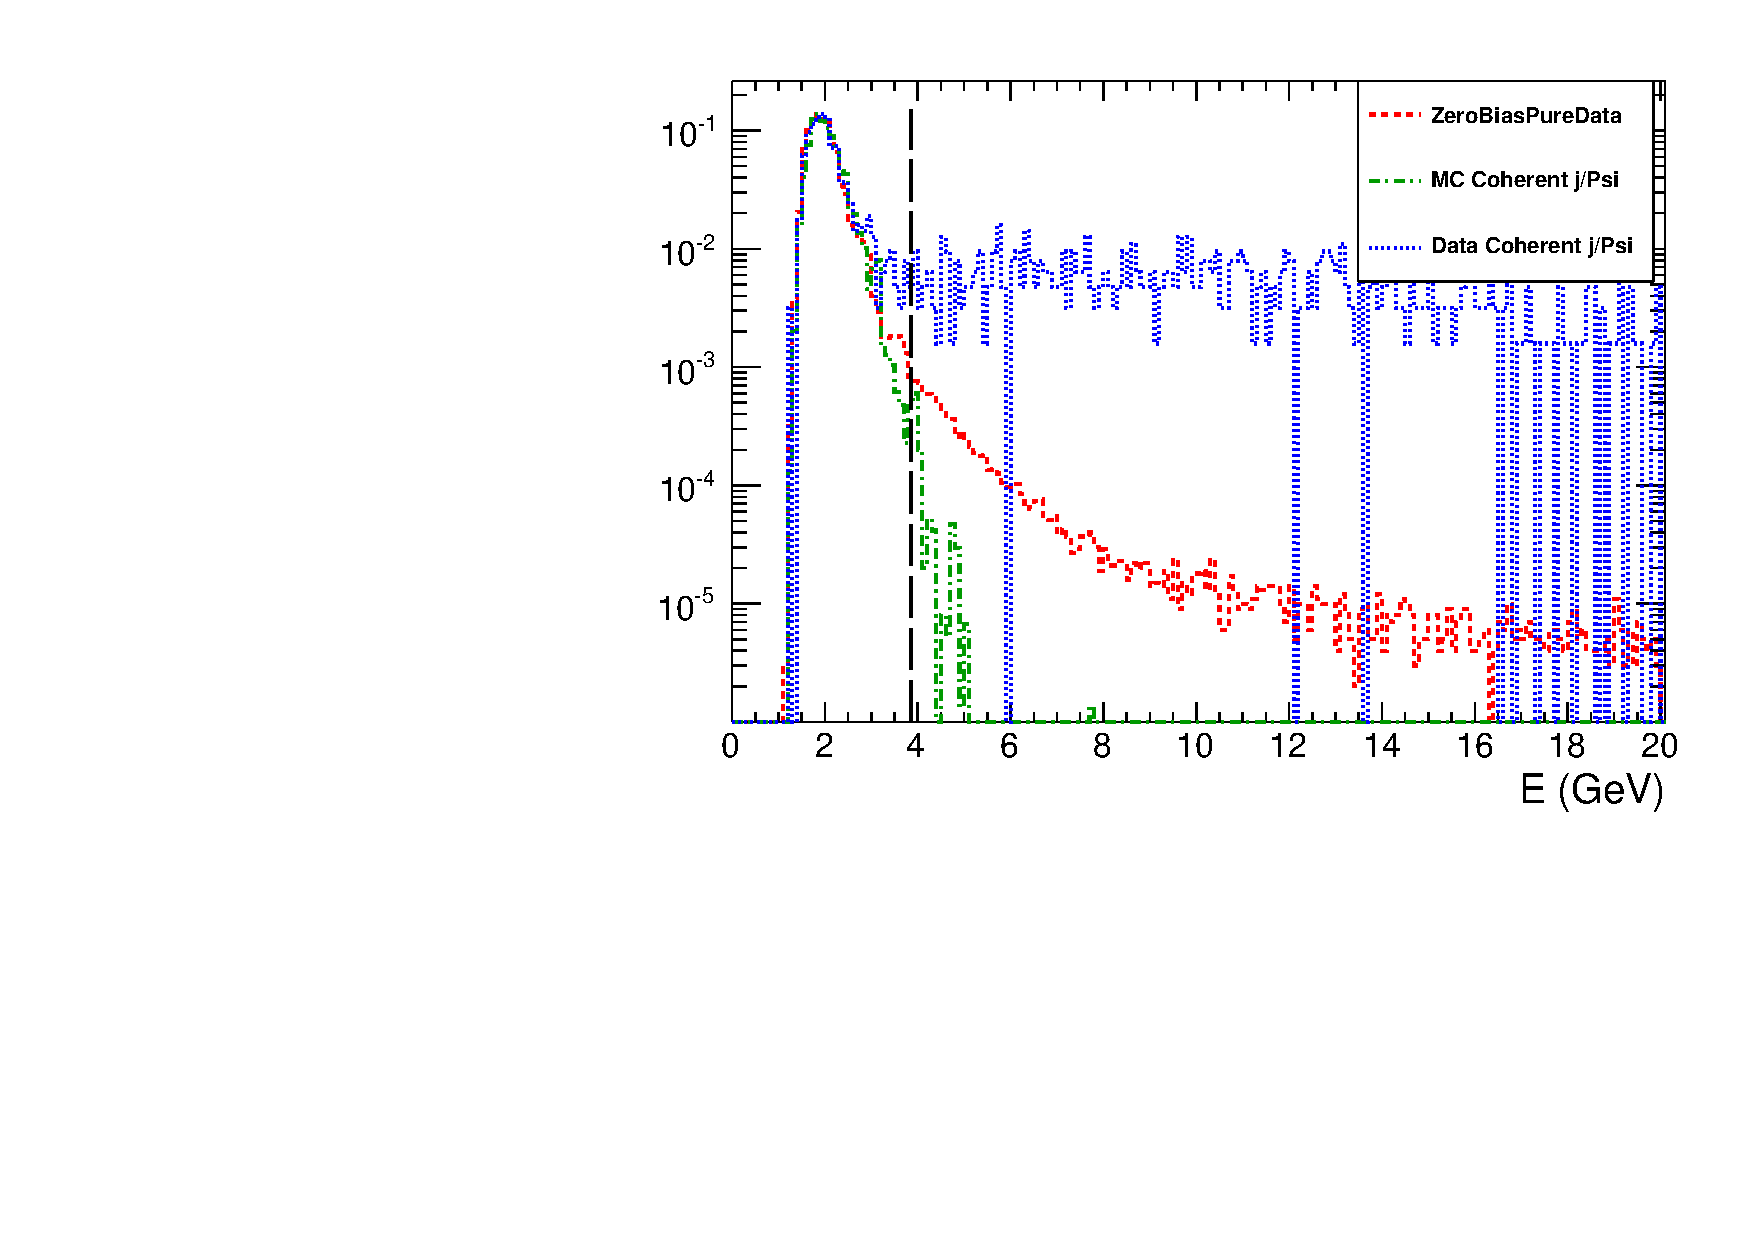
\includegraphics[width=.6\textwidth]{hfNoiseComp}
        \caption{Comparison of HF noise distributions in zero bias data, 
          physics triggered data, and MC.}
        \label{fig:hfNoiseDist}
      \end{figure}

      The following standard muon quality cuts are applied:
      \begin{itemize}
        \item Tracker track matched with at least one muon segment 
          (in any station) in both X and Y coordinates (< 3 $\sigma$).
        \item Cut on number of tracker layers with hits $>$ 5.
        \item Number of pixel layers $>$ 0.
        \item The $\chi^{2}$ per degrees of freedom of the track fit $<$ 3. 
        \item Loose transverse and longitudinal impact parameter cuts, with in 3 
          cm in the transverse direction and withing 30 cm in the longitudinal 
          direction with respect to the primary vertex.
      \end{itemize}
      These cuts are applied to reduce the number of fake muons \DIFaddbegin \DIFadd{and have been 
        validated for standard muon analyses}\DIFaddend .

  \section{\label{sec:breakUpDet} Break up determination}
    As described in Section~\ref{sec:ltaTheory}, UPC J/$\psi$ photoproduction 
      can be accompanied by the emission of neutrons from either of the two 
      colliding nuclei.
    The various neutron emission scenarios, or break-up modes, can 
      be distinguished by the ZDC.
    By separating events where the ZDC signal is consistent with 1 neutron 
      versus several neutrons, the different break-up modes can be separated
      and compared to theory. 
    For this reason, reconstruction of the ZDC signal plays an important role 
      in this thesis. 
    In order to maximize the ability to explore the one neutron peak, which 
      sits at the bottom of the ZDCs dynamic range, a new ZDC reconstruction 
      method was devised. 
    This new reconstruction method was then used to establish a one neutron and
      many neutron threshold.
    In this section the ZDC signal reconstruction is described and how the 
      neutron thresholds on this signal were set.

    \subsection{ZDC signal reconstruction}
      The ZDC signal is built up from the pulse shapes for each of the 
        18 individual ZDC channels. 
      The pulse shape is recorded in 250 ns second chunks and is divided into
        10 time slices of 25 ns (See Fig~\ref{fig:zdcPulseShape}).
      Counting from 0, the 4th time slice is synced with the timing of the rest
        of the detector and corresponds to when the products of the recorded 
        collision reached the ZDC.
      For this reason the channel signal is taken from the 4th time slice.
      \begin{figure}[h]
        \centering
        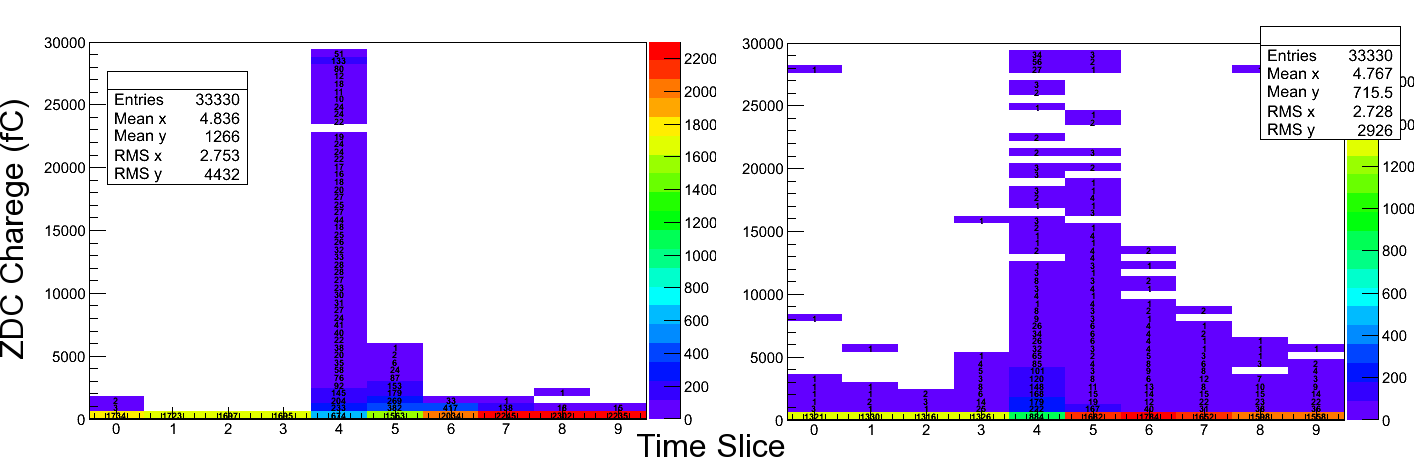
\includegraphics[width=\textwidth]{zdcPulseShape}
        \caption{Average ZDC pluse shape is plotted as the charge as a function
          of time slice for the first hadronic from ZDC$^{-}$ (left) and 
          ZDC$^{+}$ (right).}
        \label{fig:zdcPulseShape}
      \end{figure}

      The ZDC signal sits on top of a low frequency noise pedestal. 
      Over the time scale of 250 ns, this low frequency noise signal appears
        as a constant that shifts randomly from event to event.
      The contribution from this noise is therefore measured event by event
        in order to subtract it.
      Time slice 5 is used for this purpose.

      Time slices 1 and 2 could also be used to estimate the low frequency 
        noise.
      However because the noise fluctuates to negative values of charge that 
        cannot be measured, these time slices can only provide a 
        measurement of the noise half the time. 
      By using time slice 5 which contains the falling tail of the signal, 
        the noise can be measured any time the signal raises significantly 
        above the noise.
      If the fraction of signal in time slice 4 and 5 are constant and
        the noise contributes the same value to both time slices, the 
        following formula is applicable:
      \begin{equation}
        Ts4 \propto (Ts4 + C) - ( Ts5 + C ) = Ts4 - R_{Ts5/Ts4}Ts4 
        = Ts4(1-R_{Ts5/Ts4}),
        \label{eq:ts4ish}
      \end{equation}
      where $Ts4$ is the signal contribution in time slice 4, $Ts5$ is the 
        signal contribution to time slice 5, $C$ is a random noise constant
        from the low frequency noise, and $R_{Ts5/Ts4}$ is the ratio between
        the signal contribution from time slice 5 over time slice 4.
      Fig.~\ref{fig:zdcTs4OvTs5VTs5} demonstrates the consistence of the 
        fraction and validates the unconventional method of using the falling 
        tail of the signal to estimate the low frequency noise. 
      By using time slice 5, the chances of measuring the noise are maximized. 
      Separating the signal from the noise is especially important because
        the ZDC signal for the one neutron peak sits near the noise at the 
        bottom of the ZDC dynamic range.
      \begin{figure}[!Hhbt]
        \centering
        $ \begin{array}{cc}
          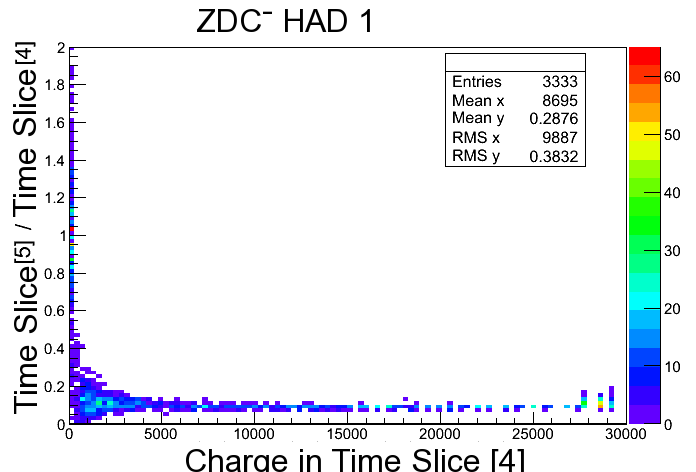
\includegraphics[width=.4\textwidth]{negTs5overTs4vts5} &
          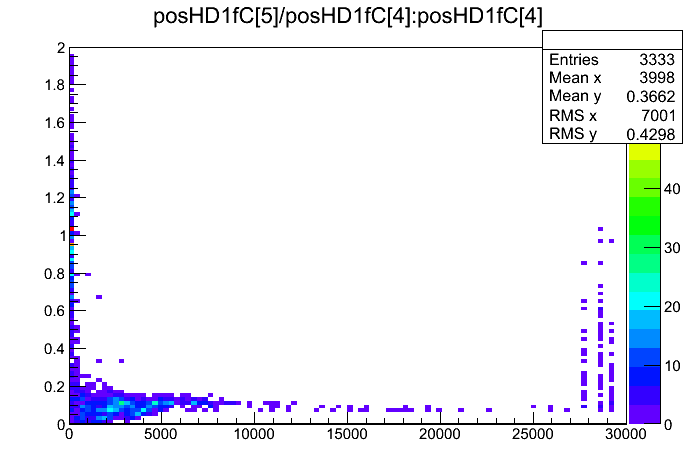
\includegraphics[width=.4\textwidth]{posTs5overTs4vts5}
        \end{array} $  
        \caption{ The fraction of signal in time slice 5 over time slice 4 
          as a function of the signal in time slice 5 in ZDC$^{-}$ (left) and 
          ZDC$^{+}$ (right).}
        \label{fig:zdcTs4OvTs5VTs5}
      \end{figure}

      To measure one signal value for ZDC$^{+}$ and one for ZDC$^{-}$, the 
        signals from each of the channels are combined.
      Channels from the EM section and HD section are combined first. 
      Only channels with signal above zero in time slice 5 and time slice 
        4 are included. 
      The EM section of the calorimeter is more densely packed with optical 
        fibers and therefore has a higher gain relative to the HAD section. 
      To account for this, the combination of EM channels is weighted with
        a factor of 0.1 to match the HAD channel gains.
      The value for each side of the ZDC's signal is given by the sum of the 
        HAD channel combination and weighted EM channel combination.
      It is this signal, one for ZDC$^{+}$ and one for ZDC$^{-}$, 
        which is plotted in Fig.~\ref{fig:zdcM2Fit} to measure the neutron 
        thresholds.

    \subsection{Determination of the one neutron thresholds}
      The ZDC thresholds used to establish the various break-up modes were 
        measured from zero bias data.
      By using this dataset, the neutron spectrum does not contain a trigger 
        bias. 
      Zero bias trigger required that both beams were present in CMS.
      This does, however, include a significant electronic noise contribution due
        to events where no neutrons are emitted in the direction of the ZDC.

      To determine the thresholds for one and multiple neutrons, the ZDC$^{+}$ 
        and ZDC$^{-}$ spectra were fit.
      Four Gaussian functions were combined to fit the spectra. 
      The electronic noise was fit to a Gaussian around zero.
      The one, two, and three neutron peaks are fit to Gaussians that are 
        successively broader.
      The mean of each peak was initially set to multiples of the mean of the 
        one neutron peak. 
      \begin{figure}[!Hh]
        \centering
        $ 
          \begin{array}{cc}
            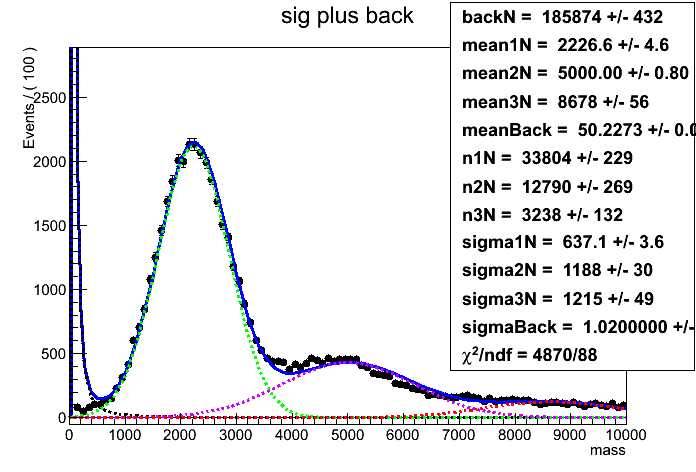
\includegraphics[width=0.45\textwidth]{zdcFit45Neg} &
            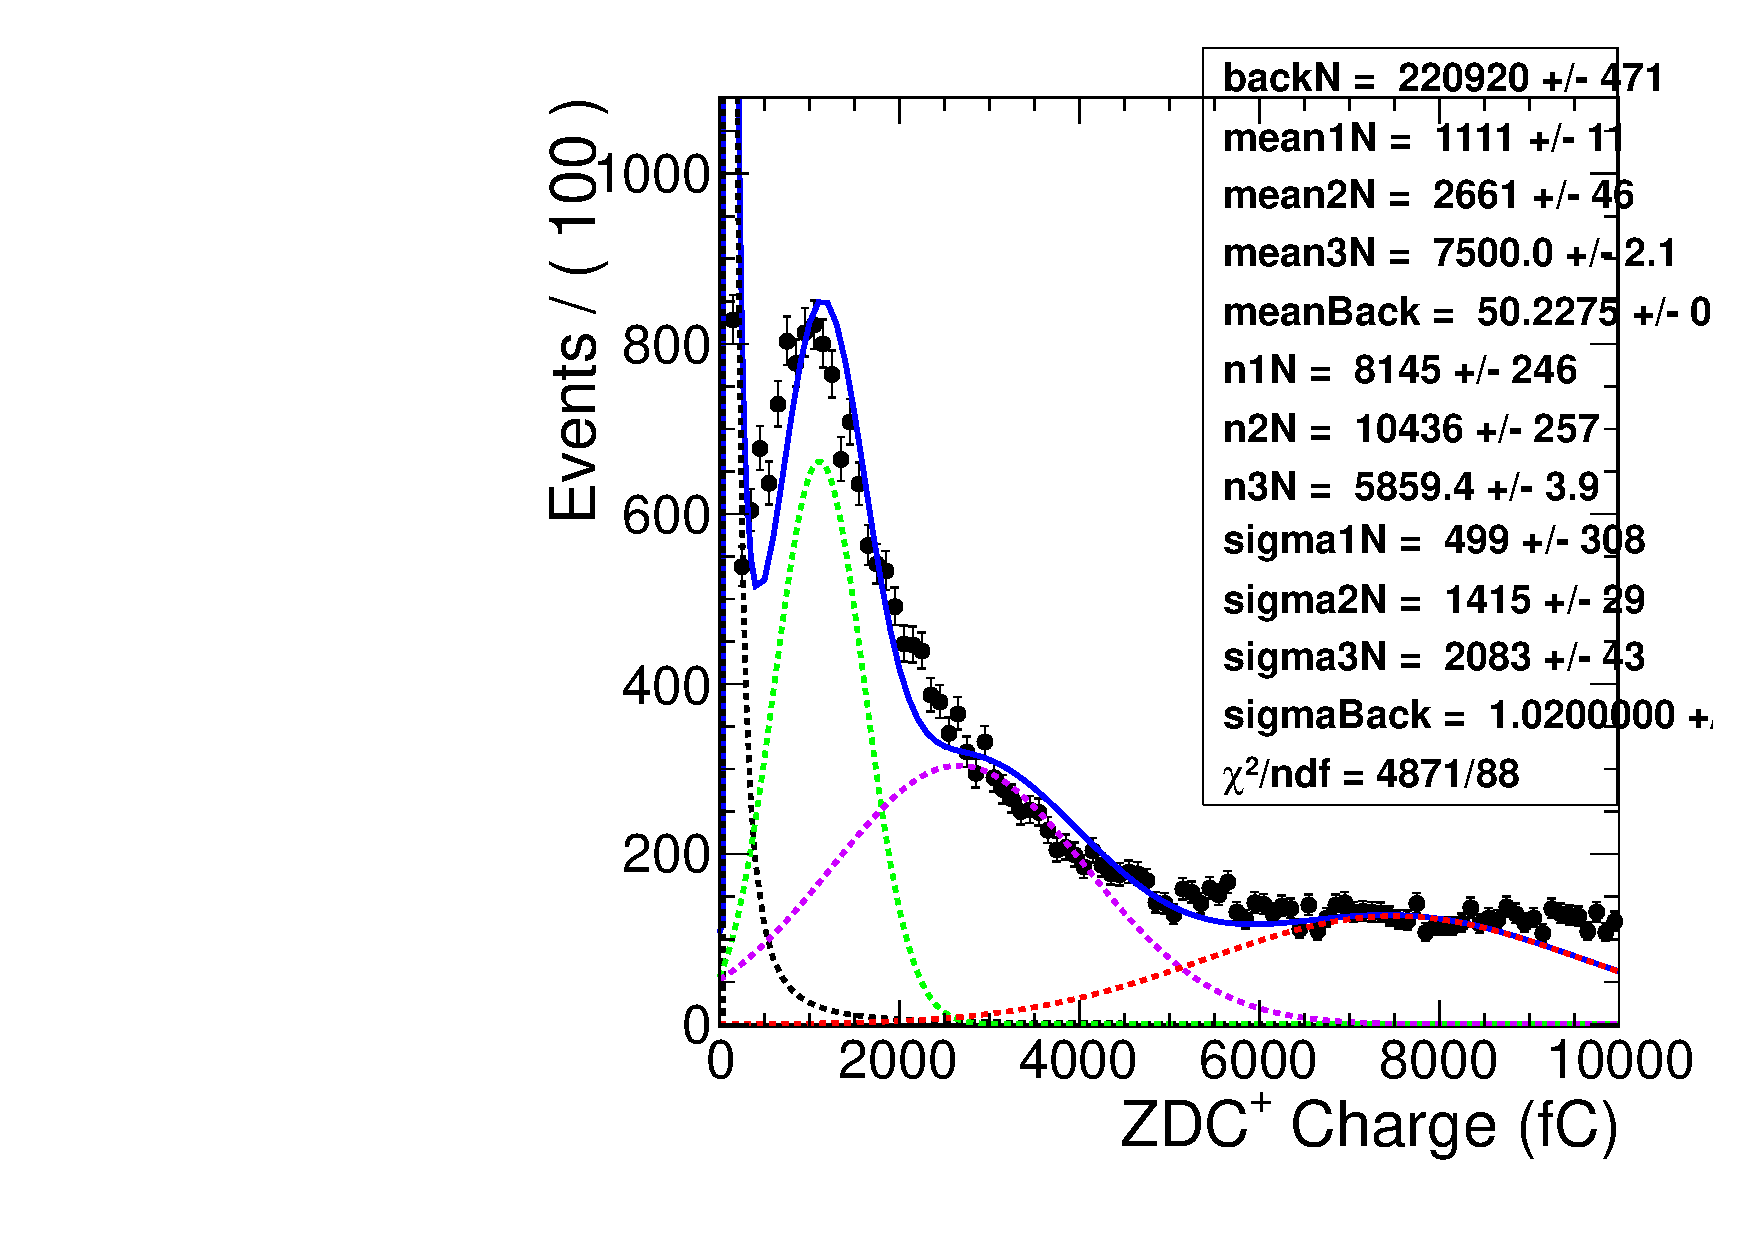
\includegraphics[width=0.45\textwidth]{zdcFit45Pos}
          \end{array} 
        $
        \caption{Fit to the signal spectra for ZDC$^{-}$ (left) and ZDC$^{+}$ 
          (right)}
        \label{fig:zdcM2Fit}
      \end{figure}
      The threshold for a neutron in the ZDC was taken from the fits in 
        Fig.~\ref{fig:zdcM2Fit}.
      Any signal greater 2$\sigma$ below the mean of the one neutron peak was 
        considered signal.
      Any signal greater than 2$\sigma$ above was considered multiple 
        neutrons.
      In this way the single neutron break up modes could be separated from the
        multiple neutron modes.

      Several of the break-up mode calculations that have been done involve
        single sided configurations where neutrons are present on one side
        of the interaction point and not the other.
      To identify signal consistent with noise, noise distributions for the 
        combined EM sections and the combined HAD sections were measured.
      The beams are only made to collide every 200 ns. 
      In Fig.~\ref{fig:zdcPulseShape} higher than average signal can be seen
        in the 0th time slice, which precedes the main signal time slice 
        time slice 4 by 200 ns. 
      This is due to events where activity was present in the ZDC for 
        two consecutive collisions.
      Time slices 1 and 2, however, occurred between collisions.
      These time slices were used to estimate the noise spectrum.
      \begin{figure}[!Hhbt]
        \centering
        $ \begin{array}{cc}
          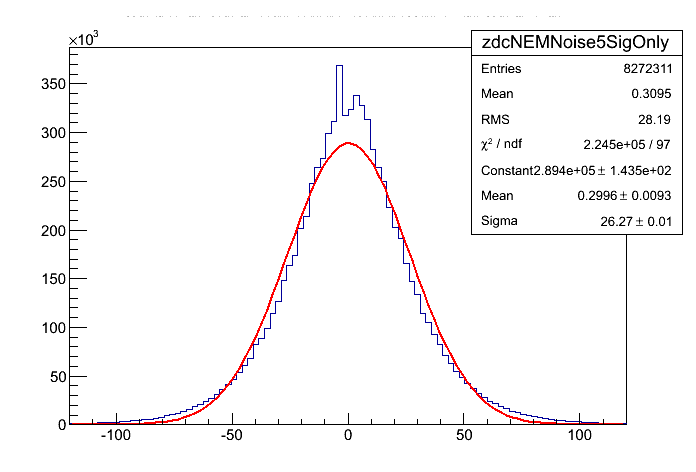
\includegraphics[width=.45\textwidth]{zdcNegEMNoiseFromZBNoCor} & 
          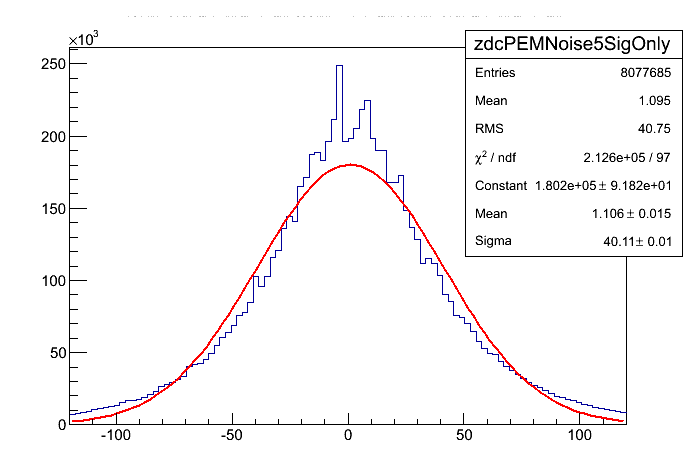
\includegraphics[width=.45\textwidth]{zdcPosEMNoiseFromZBNoCor} \\
          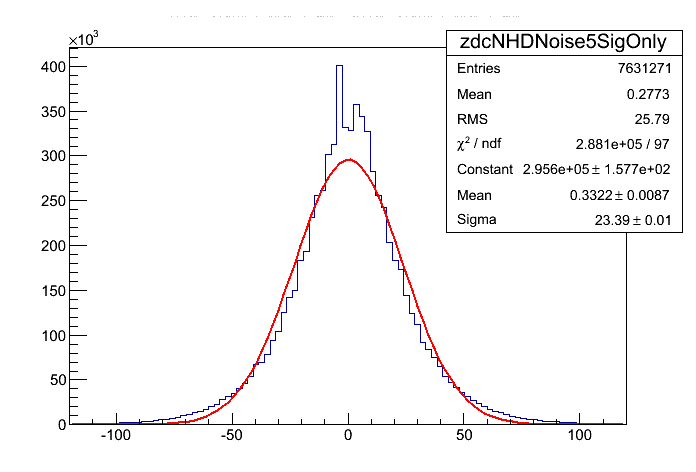
\includegraphics[width=.45\textwidth]{zdcNegHDNoiseFromZB} &
          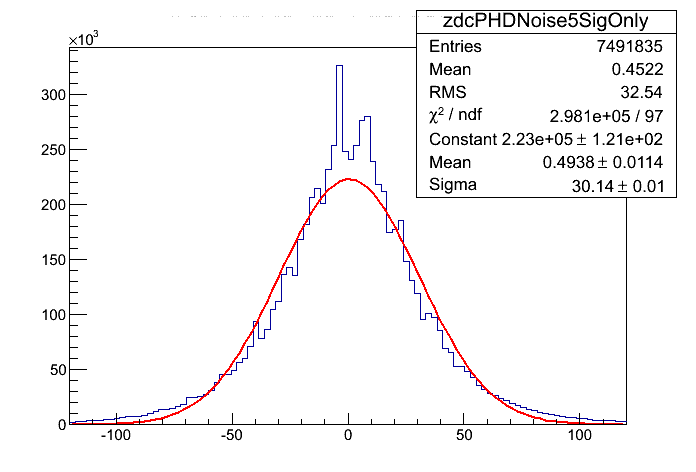
\includegraphics[width=.45\textwidth]{zdcPosHDNoiseFromZB}
        \end{array} $
        \caption{ZDC noise spectra from ZDC$^{-}$ EM section (upper left), 
          ZDC$^{+}$ EM section (upper right), ZDC$^{-}$ HAD section (lower left), 
          and ZDC$^{+}$ HAD section (lower right).}
        \label{fig:zdcNoiseSpectra}
      \end{figure}

      Fig~\ref{fig:zdcNoiseSpectra} shows the noise spectrum for each of the 
        EM and HAD sections for the two sides of the ZDC. 
      As with the signal measurements, the low frequency noise pedestal is 
        subtracted event by event by subtracting time slice 2 from time slice
        one before the channel signals are combined for each section.
      A side is considered consistent with noise if both HAD section and EM 
        section signal measurements from the signal method involving time slice
        4 and time slice 5 are lower than 2 sigma below the mean in 
        Fig.~\ref{fig:zdcNoiseSpectra}.
      With the single neutron, multi-neutron, and noise thresholds established,
        the contributions to the various break-up modes were estimated and 
        compared to theory. 


  \section{\label{sec:sigEx} Signal extraction}
    After all event selection cuts, the coherent J/$\psi$, incoherent J/$\psi$,
      and photon-photon process all contribute to the remaining events.
    Each process must be separated from the final mix.
    To achieve this, the invariant mass and $p_{T}$ distributions are used 
      to distinguish between the three processes. 
    The photon-photon process is extended in invariant mass whereas the 
      J/$\psi$ is peak strongly near 3.1 GeV.
    In $p_{T}$ the photon-photon and coherent process have similar 
      distributions, both peaked shapely below 0.1 GeV, whereas the incoherent 
      process is more broadly distributed across an interval extending to 
      nearly 1 GeV.
    The mass distribution was \DIFdelbegin \DIFdel{fitted }\DIFdelend \DIFaddbegin \DIFadd{fit }\DIFaddend to separate the photon-photon process from
      the J/$\psi$ process.
    The $p_{T}$ distribution was used to separate the incoherent process from 
      the photon-photon process, and the coherent process. 
    In this way, a separate yield was extracted for all three processes. 

    The invariant mass distribution for opposite sign dimuons is shown in 
      Fig.~\ref{fig:massFit}. 
    A J/$\psi$ signal is clearly visible together with tails at higher and
      lower mass due to the photon-photon process.
    A fit to the invariant mass distribution was done using a Gaussian
      to account for the J/$\psi$ signal and a first order polynomial function 
      for the photon-photon process.
    The extracted number of J/$\psi$ candidates from this fit includes all 
      J/$\psi$s in the mass window that passed the analysis cuts, i.e. both
      coherent and incoherent process contribute to yield from the mass
      fit.
    The $p_{T}$ distribution is needed to separate the two different 
      contributions to the J/$\psi$ peak. 

    \begin{figure}[!Hhtb]
      \centering
      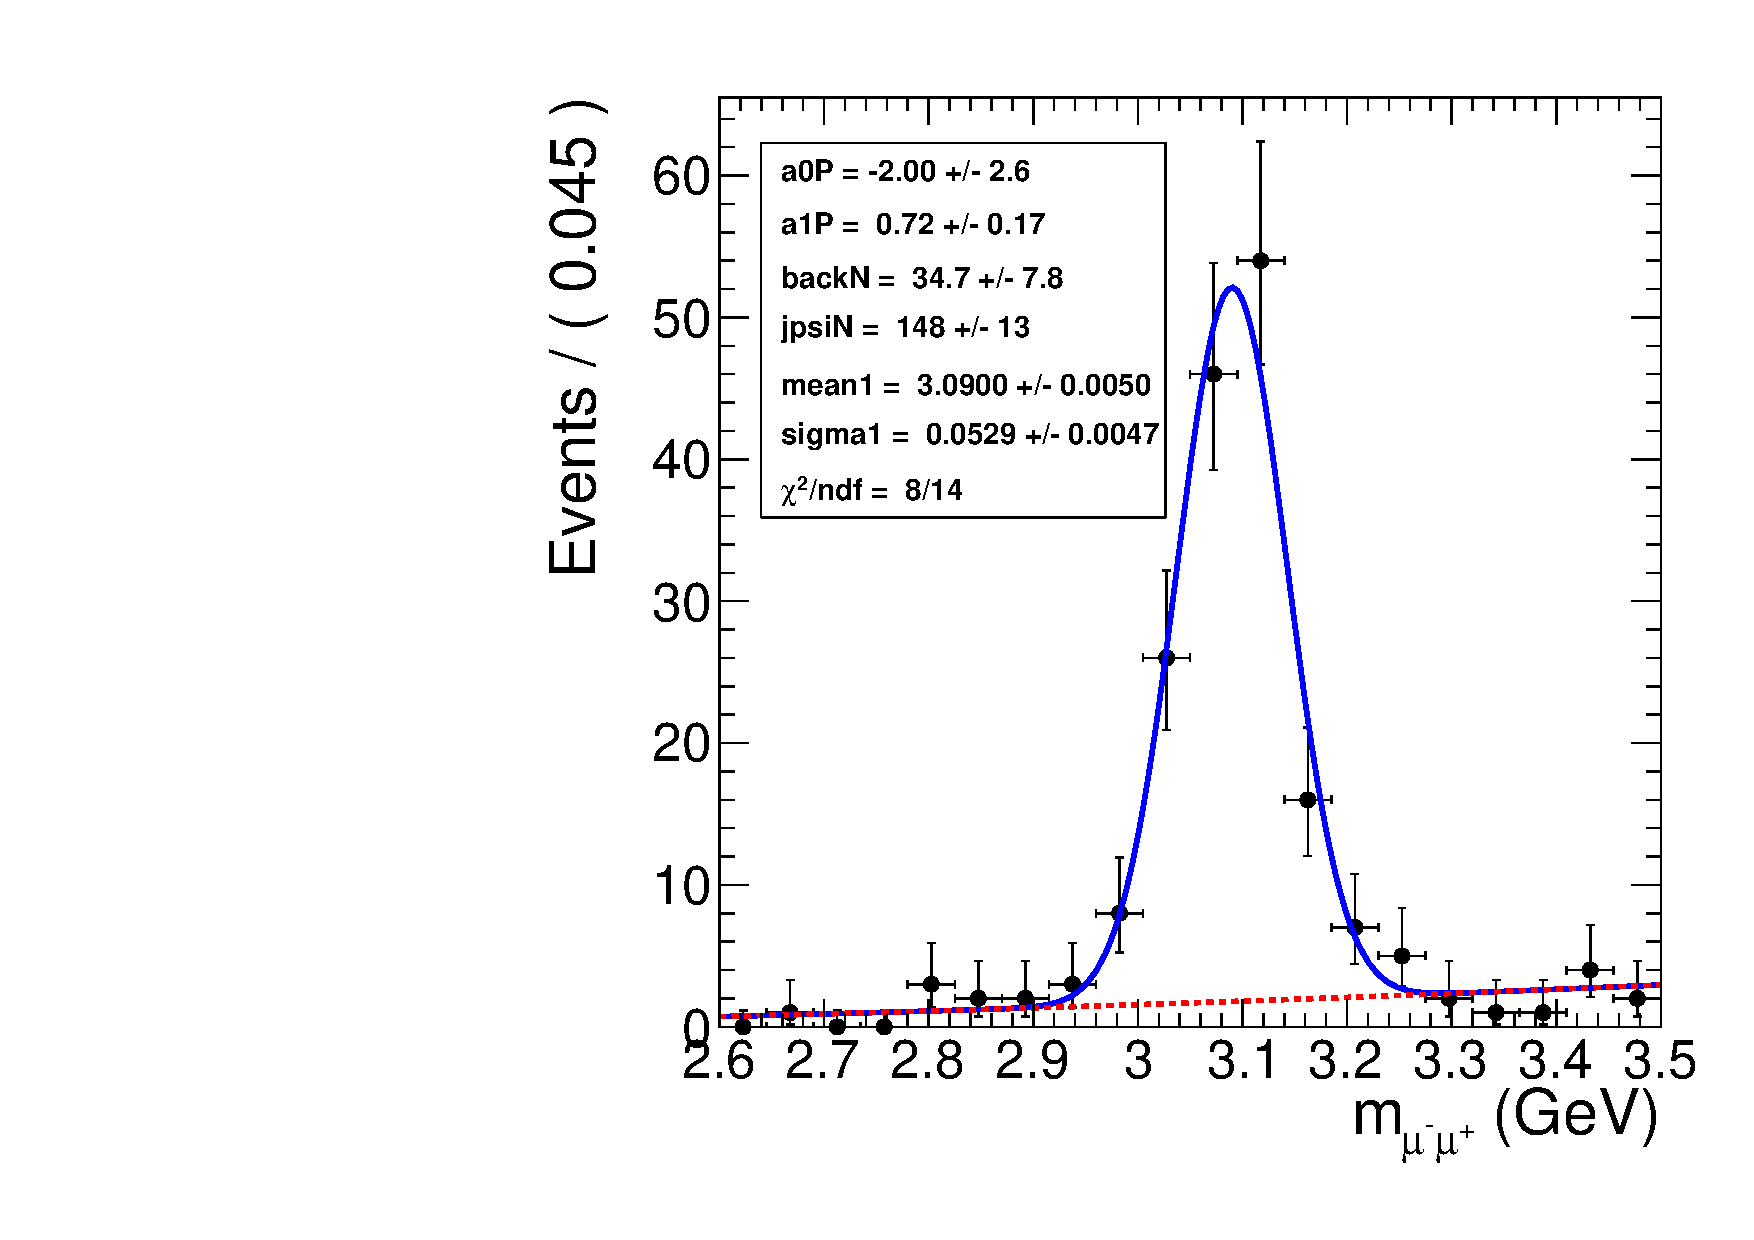
\includegraphics[width=.6\textwidth]{massFitSimple}
      \caption{Mass fit to J/$\psi$ using Gaussian for the 
        signal and a first order polynomial for the photon-photon continuum}
      \label{fig:massFit}
    \end{figure}

    The same candidates from Fig.~\ref{fig:massFit} were plotted as a function
      of $p_{T}$ in Fig.~\ref{fig:ptTemps}.
    The clear overlap of the coherent and photon-photon process, and the 
      clear separation of these two lower $p_{T}$ processes from the incoherent
      process is apparent.
    The shape of the $p_{T}$ distribution for the coherent, incoherent, and 
      photon-photon process are taken from the final output of MC after
      applying all analysis cuts. 
    To obtain the yields for each of the three process, the $p_{T}$ 
      distribution was fit to the three templates.
    In Fig.\ref{fig:ptTemps}, the yield parameters that were fit were left
      unconstrained for all three process.

    \begin{figure}[!Hhbt]
      \centering
      \includegraphics[width=.6\textwidth]{ptOnly}
      \caption{ Fit to MC $p_{T}$ templates. }
      \label{fig:ptTemps}
    \end{figure}

    The shape of the photon-photon and coherent J/$\psi$ process are very 
      similar in $p_{T}$.
    Accordingly, the contribution from the photon-photon process and the 
      coherent process are difficult to separate from the $p_{T}$ distribution.
    The confidence contours in Fig.~\ref{fig:ptOnlyCor} from the template fit
      in Fig.~\ref{fig:ptTemps} demonstrate the strong anti-correlation 
      between the coherent yield parameter, $nCo$, and the yield parameter 
      for the photon-photon process, $nGamma$.
    Because of the anti-correlation, the statistical uncertainty on $nCo$ and 
      $nGamma$ from the fit are larger than $\sqrt{nCo}$ and $\sqrt{nGamma}$
      expected from Poisson statistics. 
    The information from the invariant mass and $p_{T}$ distributions were
      combined to break this correlation. 
    Through this combination, the contribution to the final yield from 
      the three process was measured.

    \begin{figure}[!Hhbt]
      \centering
      \includegraphics[width=.6\textwidth]{nCoNGammaCorPtOnly}
      \caption{68\%, 95\%, and 99\% confidence contours from the $p_{T}$ 
        template fit. }
      \label{fig:ptOnlyCor}
    \end{figure}

    To utilize the mass fits ability to distinguish the photon-photon process 
      from the coherent and incoherent process all while utilizing the $p_{T}$
      fits ability to separate the coherent and photon-photon processes from 
      the incoherent, a simultaneous fit to the mass spectrum and $p_{T}$ 
      spectrum was preformed.
    Fig.~\ref{fig:simFitMassPtGauss} shows the result of the simultaneous fit.
    The simultaneous fit forces the parameter $nGamma$ to both describe the 
      photon-photon continuum present in the side bands of the J/$\psi$ mass 
      peak as well the photon-photon contribution to the low-$p_{T}$ part of 
      the $p_{T}$ spectrum.
    In addition, the J/$\psi$ yield from the mass fit is forced to equal the
      contribution from the incoherent and coherent process in the 
      fit to the $p_{T}$ distribution. 
    In this way, the correlation between the yield parameters was broken, and 
      the contribution from the three process were made independent of each 
      other.

    \begin{figure}[!Hhbt]
      \centering
      \includegraphics[width=0.9\textwidth]{ptMassSimGaussLine}
      \caption{Simultaneous fit to the mass and $p_{T}$ spectra.}
      \label{fig:simFitMassPtGauss}
    \end{figure}

    The ambiguity between the coherent and incoherent processes in the mass fit
      and the ambiguity between the coherent and the photon-photon process was 
      over come through used of the simultaneous fit.
    Fig.~\ref{fig:simGaussCor} shows the confidence contours for $nCo$ and 
      $nGamma$ from the simultaneous fit in Fig.~\ref{fig:simFitMassPtGauss}.  
    The slope of the confidence contours in Fig.~\ref{fig:simGaussCor} 
      is noticeably closer to 0 than the apparent negative slope in 
      Fig.~\ref{fig:ptOnlyCor}.
    The contours for the simultaneous fit are also reduced compared to 
      Fig.~\ref{fig:ptOnlyCor} with widths in $nCo$ and $nGamma$ similar to 
      those expected from Poison statistics. 
    From the simultaneous fit, reasonable statistical errors were obtained 
      along with the yields for the three processes. 

    \begin{figure}[!Hhbt]
      \centering
      \includegraphics[width=0.6\textwidth]{nCoNGammaCorPtMass}
      \caption{68\%, 95\%, and 99\% confidence contours from the 
        simultaneous fit. }
      \label{fig:simGaussCor}
    \end{figure}

  \section{\label{sec:effDet} Efficiency determination}
    \subsection{Muon efficiencies}
      The muon efficiencies are measured from MC and data.
      The MC based measurement accounts for the detector acceptance and the 
        efficiency of the muon quality discussed in 
        Section~\ref{sec:DataSetEvSel}.
      The trigger efficiencies were measured in data using the tag and probe 
      method \cite{cmsTnP}, which is discussed below. 

       CMS has a limited acceptance for J/$\psi$s, particularly in the case of 
        J/$\psi$s with low momentum like those produced in UPC events. 
      To measure the acceptance of CMS for J/$\psi$s, reconstructed dimuon 
        candidates were considered detectable if both reconstructed daughters 
        fell into a detectability region.
      This region was defined using the coherent J/$\psi$ events obtained from 
        STARlight.
      The efficiency for reconstructing single muons $\varepsilon^{\mu}_{reco}$ 
        is defined by $\varepsilon^{\mu}_{reco} = \frac{N^{\mu}_{reco}}{N^{\mu}_{gen}}$, 
        where $N^{\mu}_{reco}$ is the number reconstructed muons obtained 
        after the full CMS detector simulation and that passed the standard
        muon quality cuts, and $N^{\mu}_{gen}$ is the number of generated 
        muons from STARlight.
      \begin{figure}[!Hhtb]
        \centering
          \includegraphics[width=.6\textwidth]{mcEffMaps/accMuJpCo} 
        \caption{ Muon daughter detectability from coherent J/$\psi$}
        \label{fig:muonDaughterDet}
      \end{figure}
      Fig.~\ref{fig:muonDaughterDet} shows the efficiency for reconstructing
        single muons from coherent J/$\psi$ events.
      To avoid the edges of the detectors acceptance, all reconstructed muons 
        that fall into a ($p_{T}$,$|\eta|$) bin that has an efficiency less 
        than 20\% were rejected thus defining the detectability region.
      The acceptance for reconstructing dimuons was calculated from MC
        using the following formula:
      \begin{equation}
        A=\frac{N_{det}(|y|,p_{T})}{N_{gen}(|y|,p_{T})},
        \label{eq:jpsiAccEq}
      \end{equation}
        where $N_{det}$ is the number of reconstructed dimuons where both 
        daughters fall into the detectability region, and $N_{gen}$ is the
        number of generated dimuons. 
      From Eq.~\ref{eq:jpsiAccEq}, the acceptance for J/$\psi$ was calculated
        as a function of $|y|$, and $p_{T}$ (see Fig.~\ref{fig:jpsiAcceptance}).
        \begin{figure*}[!Hhtb]
          \centering
          $ \begin{array}{cc}
            \includegraphics[width=.45\textwidth]{mcEffMaps/detAccJpCoStep} &
            \includegraphics[width=.45\textwidth]{mcEffMaps/detAccJpInCoStep} \\
            \includegraphics[width=.45\textwidth]{mcEffMaps/detAccGammaStep}
          \end{array} $
          \caption{Dimuon acceptance from coherent J/$\psi$ (top left), incoherent 
            J$\psi$ (top right), and photon-photon interactions (lower).}
          \label{fig:jpsiAcceptance}
        \end{figure*}

      The tag and probe method is used to measure the trigger efficiency of 
        the muon daughters, which is a data driven approach. 
      In this method there are three categories of daughter muons. 
      \textit{Tag muons} are high quality muons.
      \textit{Passing probes} are reconstructed muons that match the muon trigger, 
        while \textit{failing probes} do not. 
      Each dimuon will have one daughter classified as a tag and the other
        as a probe.
      From here three invariant mass histograms are studied. 
      One histogram is created from all pairs. 
      The second comes from pairs where the probe is a passing probe.  
      The last histogram comes from pairs where the probe fails to fulfill
        the trigger, \textit{i.e.} the probe is a failing probe. 
      Because this depends on the $p_{T}$ and $|\eta|$ of the probe, one set 
        of three histograms for each ($p_{T}$,$|\eta|$) bin of the probe is 
        created.

      To extract the single muon trigger efficiency $\varepsilon^{\mu}_{trig}$, 
        each set of invariant mass histograms was simultaneously fitted. 
      The signal was fitted using a Crystal Ball function, and the background 
        was fitted to an exponential.
      The Crystal Ball parameters were simultaneously fitted to all three 
        histograms.
      The exponential function was fitted to the failing and passing probe 
        histograms separately.
      Because the background shapes are in principle different for the two 
        samples, the efficiency is driven by this difference. 

      To measure the trigger efficiency a tag is required to pass all muon
        quality cuts and matched to the trigger.
      The probe is required to pass all quality cuts. 
      A passing probe is a probe that is also matched to the trigger. 
      In this way, the tag leaves the probe unbiased by the trigger and the 
        efficiency can be measured by fitting the mass distribution.  

      Fig.~\ref{fig:tnpFitPlot} shows the fit of the three sets of pairs. 
      \begin{figure}[!Hh]
        \centering
        \includegraphics[width=.6\textwidth]{tNp/tnpFits}
        \caption{Fits to tag and probe pairs in the J/$\psi$ mass region.}
        \label{fig:tnpFitPlot}
      \end{figure}
      This fit is done for each bin of the probes $p_{T}$ and $\eta$.
      The resulting fit is in Fig.~\ref{fig:tnpTrigMap}.
      \begin{figure}[!Hhbt]
        \centering
        \includegraphics[width=.6\textwidth]{tNp/tnpFromFit}
        \caption{Muon trigger efficiencies in $p_{T}$ and $\eta$ bins from 
          the tag and probe method.}
        \label{fig:tnpTrigMap}
      \end{figure}

      The dimuon trigger efficiency $\varepsilon^{dimuon}_{trigger}$ was measured
        from the single muon efficiencies. 
      The efficiency of each candidate was calculated using the following
        equation:
      \begin{equation}
        \label{eq:dimuTrigEff}
        \varepsilon^{dimuon}_{trigger}=1-(1-\varepsilon_{trigger}^{\mu_{1}})(1-\varepsilon_{trigger}^{\mu_{2}}),
      \end{equation}
      where $\varepsilon_{trigger}^{\mu_{1}}$ is the tag and probe efficiency
        of the first dimuon daughter, and $\varepsilon_{trigger}^{\mu_{2}}$ is
        the efficiency of the second muon daughter. 
      In Eq.~\ref{eq:dimuTrigEff} the probability of at least one daughter
        firing the trigger is calculated by subtracting one from the
        probability that neither daughter fires the trigger,
        thus giving the dimuon trigger efficiency. 

      The average dimuon trigger efficiency for each dimuon ($p_{T}$,$|y|$) bin
        was calculated by averageing the individual dimuon candidates in each
        bin. 
      \begin{figure}[!Hhbt]
        \centering
        \includegraphics[width=0.6\textwidth]{averageTriggerEff}
        \caption{The trigger efficiency from tag and probe averaged over candidates
          in each ($p_{T}$,$|y|$) bin.}
        \label{fig:avTrigEffCo}
      \end{figure}
      The average trigger efficiency was multiplied by the acceptance from the MC 
        to produce a total factor for both efficiency and acceptance. 
      \begin{figure}[!Hhtb]
        \centering
        \includegraphics[width=0.6\textwidth]{averageExA}
        \caption{The acceptance times averaged trigger efficiency from tag and 
          probe.}
        \label{fig:avAccEff}
      \end{figure}

      The total combined efficiency and acceptance factor coherent J/$\psi$ 
        between 2.0 < |y| 2.2 was found to be around 5\%.
      The roughly 7\% acceptance factor from the MC is the main contributor
        to the total efficiency. 
      Primarily, the interplay of the polarization of the J/$\psi$ and
        the material in detector drive down the efficiency by creating an 
        effective momentum threshold for detection (see 
        Section~\ref{sec:mcSim}).
      The reconstruction efficiency of the daughters \DIFdelbegin \DIFdel{is ranges }\DIFdelend \DIFaddbegin \DIFadd{range }\DIFaddend between 
        20\%-60\% for muons in the defined detectability range. 
      The trigger efficiency for the detectable muons ranges from 30\%-80\% 
        depending on $p_{T}$. 
      The typical trigger efficiency for the dimuons \DIFdelbegin \DIFdel{was just over }\DIFdelend \DIFaddbegin \DIFadd{ranges from }\DIFaddend 60\% \DIFaddbegin \DIFadd{to 80\%}\DIFaddend .

    \subsection{ZDC trigger efficiency}
      As discussed in Section~\ref{sec:breakUpDet}, a special trigger was 
        prepared to monitor the ZDC trigger efficiency. 
      This trigger required either a ZDC$^{+}$ or ZDC$^{-}$ trigger, together with at 
        least one pixel track. 
      Events were accepted offline if there was no activity in the BSCs or 
        activity on a single side. 

      This sample suffers from a trigger bias. 
      For example, a sample triggered by ZDC$^{+}$ would always produce a ZDC$^{+}$ 
        trigger efficiency of one. 
      To avoid this, the special trigger sample was divided into two 
        subsamples in the following way. 
      A first sample triggered by the ZDC$^{+}$ input and second one triggered by 
        the ZDC$^{-}$. 
      The ZDC$^{+}$ trigger efficiency is measured from the ZDC$^{-}$ sample, and vice 
        versa.

      The trigger efficiency for reconstructed ZDC energies above the
        single neutron threshold were estimated (see for Sec.~\ref{sec:breakUpDet}).
      The ZDC$^{+}$ efficiency was calculated using the ZDC$^{-}$ triggered 
        sample.
      To estimate the efficiency, the number of events with energy in 
        ZDC$^{+}$ greater than the single neutron threshold, N$_{events}$, 
        were measured.
      From this set of events, the number of events that also fire the 
        ZDC$^{+}$ was measured.
      The ratio between the number of single neutron events that fired the 
        trigger and all single neutron events was taken as the estimate of 
        trigger efficiency. 
      The same procedure was applied for each side of the ZDC.
      The trigger efficiency of the ZDC was found to be 98\% for ZDC$^{-}$
        and 94\% for ZDC$^{+}$.

      \begin{table}
        \centering
        \begin{tabular}{|c|c|c|c|c|}
           ZDC Side & Reco Method & N$_{events}$ & N$_{trig}$ & $\varepsilon_{ZDC}$ \\ \hline
           ZDC$^{+}$ & 1 & 72946  & 71688 & 0.982 $\pm$ 0.005 \\ \hline
           ZDC$^{+}$ & 2 & 73028  & 71706  & 0.9819  $\pm$ 0.005  \\ \hline
           ZDC$^{-}$ & 1 & 76137  & 71786  & 0.9429  $\pm$ 0.005  \\ \hline
           ZDC$^{-}$ & 2 & 76132  & 71859  & 0.9439  $\pm$ 0.005  \\ \hline
        \end{tabular}
        \caption{ZDC trigger efficiencies for ZDC reconstruction method 1 and 
          2}
        \label{tab:zdcEfficiency}
      \end{table}

  \section{\label{sec:sysCheck} Systematic checks}

    Table~\ref{tab:sumsyst} shows the systematic errors that were estimated.
    The method used to separate the coherent from the photon-photon process 
     is the most dominant error.
    The ZDC reconstruction method used to estimate the neutron thresholds 
      is the next most dominant, followed by the method used to estimate
      the HF noise threshold. 

    \begin{table}[!Hhtb]
      \begin{center}
        \begin{tabular}{|c|c|c|}
          \hline
          systematic & uncertainty in \%  \\ \hline
          Template fit normalized & +9.5\% -12\%    \\ \hline
          ZDC reconstruction  & 2.9\%  \\ \hline
          ZDC trigger efficiency & 2.2\%    \\ \hline
          HF noise threshold & +1.3\% -3.4\%    \\ \DIFaddbeginFL \hline 
          \DIFaddendFL MC acceptance & 1.1\%    \\ \hline
          \hline \hline
          Total systematic & 8.1\%    \\ \hline
        \end{tabular}
        \caption{Summary of systematic uncertainties}
        \label{tab:sumsyst}
      \end{center}
    \end{table}

    \subsection{HF noise threshold}
      The way in which the HF noise distribution is measured effects the event 
        selection and therefore the final candidate yeild.
      This cut plays a significant role in rejecting hadronic events.
      In Table~\ref{tab:evSelCutNumbers} the importance of cutting on HF noise
        is evident. 
      The HF noise cut rejects a little less than 1/5 of the remaining events. 
      The systematic uncertainties on the HF noise requirement is important for
        this reason.
      The result must not depend significantly on the method used to apply the
        cut on the noise because of the large reduction of events that result
        from it. 

      Four different approaches were employed to estimate the systematic effect
        arising from picking a particular method for setting the HF noise
        threshold. 
      By looking at the variation of the number of events that remain after 
        applying the thresholds derived from these four methods, the systematic
        uncertainty for the HF noise cut was estimated.
      The four methods are derive from combinations of two variations. 
      The type of object was varied from a low-level detector object called a 
        RecHit to a higher level physics object called a CaloTower. 
      The RecHit is the energy deposited in a single calorimeter detector 
        element, where as the CaloTower is a collection of RecHits with 
        varrious threholds, which represent a full energy deposit that would 
        come from a particle or a collection of particles from a jet passing 
        through the detector. 
      The second variation is on the separation of the two sides.
      In one case the threshold is derived for the two sides combined.
      In another case the thresholds are calculated separately for the two 
        sides of HF.
      By combining these two variations, a total of four estimates of the 
        effect of the HF noise cut were made.
      Table~\ref{tab:hfNoiseThreshAsym} below shows the thresholds that are 
        measured for each of the four methods.
      The resulting yields from the four different methods are displayed in 
        Table~\ref{tab:hfCutYieldEffects}.

      \begin{table}[!Hhbt]
        \centering
        \begin{tabular}{|c|c|c|c|}
          \hline
          Object type & HF (GeV) & HF$^{-}$ (GeV) & HF$^{+}$ (GeV) \\ \hline
          RecHits & 3.85 & 3.25 & 3.45 \\ \hline
          CaloTowers & 4.25 & 3.25 & 3.75 \\ \hline
        \end{tabular}
        \caption{HF noise theresholds for various noise measurement methods.}
        \label{tab:hfNoiseThreshAsym}
      \end{table}

      \begin{table}[!Hhbt]
        \centering
        \begin{tabular}{|c|c|c|}
          \hline
          Object type & Combinded HF threshold & Two-sided thresholds \\ \hline
          RecHits & 298 & 290 \\ \hline
          CaloTowers & 302 & 288 \\ \hline
        \end{tabular}
        \caption{Candidate yields below 1.05 GeV $p_{T}$ for various HF noise
          cuts.}
        \label{tab:hfCutYieldEffects}
      \end{table}

      The threshold was adjusted to estimate the effect of tightening the
        requirement on the zero bias data.
      By successively lowering the percentage of the zero bias sample
        that was included, the HF noise cut was made more restrictive including
        first 98\%, than 97\% of all zero bias events. 
      This was done for both object types, RecHits and CaloTowers.
      This allows for an estimate of the systematic uncertainty on selecting 
        a 99\% cut.
      Table~\ref{tab:hfAdjustedThresholds} shows the effect on the thresholds
        themselves for both RecHits and CaloToweres, whereas 
        Table~\ref{tab:hfAdjThreshYields} shows the effect on the candidate 
        yields.

      \begin{table}[!Hhbt]
        \begin{center}
          \caption{Values of the energy cuts for the HF calorimeter for RecHit and CaloTower in GeV.}
          \label{tab:hfAdjustedThresholds}
          \begin{tabular}{|c|c|c|} \hline
            \% &  $E_{RecHit}$ GeV & $E_{CaloTower}$ GeV\\ 
            \hline
            99 & 3.85& 4.25 \\ \hline
            98 & 3.25& 3.75 \\ \hline
            97 & 2.95& 3.25 \\  \hline
           \end{tabular}
         \end{center}
      \end{table}

      \begin{table}[!Hhbt]
        \begin{center}
          \caption{Number of dimuon candidates with  p$_{T} <$1.05 when changing HF calorimeter cuts for RecHit and CaloTower.}
          \label{tab:hfAdjThreshYields}
          \begin{tabular}{|c|c|c|} \hline
            \% &  RecHit cut & CaloTower cut\\ \hline
            99 &   298 & 302 \\ \hline
            98 &  287  & 294 \\ \hline
            97 & 284 & 280 \\ \hline
          \end{tabular}
        \end{center}
      \end{table}

      The systematic uncertainty in the HF noise threshold measurement was 
        calculated taking the difference from the 99\% combined RecHit method
        with the upper and lower extrema. 
      The systematic uncertainty from this method is calculated to be +1.3\% 
        -3.4\%.


    \subsection{Template fit normalization}
      \begin{figure}[!Hhtb]
        \centering
        \includegraphics[width=.6\textwidth]{ptOnly}
        \caption{Coherent, incoherent, and photon-photon process $p_{T}$ template fit to data.}
        \label{fig:ptTempFit}
      \end{figure}

      The $p_{T}$ template fit depends on the functions chosen for the fit
        to the mass distribution.
      As described in Section~\ref{sec:sigEx}, the similarity of the of the 
        $p_{T}$ distribution for the coherent and photon-photon process make
        the contributions from the two process difficult to separate from the 
        $p_{T}$ distribution alone.
      The mass distribution was used to distinguish between these two processes.
      In turn, the $p_{T}$ becomes dependent on the mass fit. 

      The systematic uncertainty due to the choose of functions used to fit
        the mass distribution was estimated by varying the signal and 
        background functions.
      The contribution to the background from the mass fit was used to fix the
        contribution from the photon-photon process in the $p_{T}$ template
        fit.
      Two functions were used to describe the signal, a Gaussian, and a Crystal
        ball function. 
      The background was fit to a linear function, a 2nd order polynomial, and
        a 2nd order Cheby-Chev polynomial. 
      The resulting variation on the coherent contribution was used to as an
        estimate of this systematic effect. 

      \begin{figure}[!Hhbt]
        \centering
        $ \begin{array}{ccc}
          \includegraphics[width=.3\textwidth]{cbPolyBkgEst} &
          \includegraphics[width=.3\textwidth]{gausLinBkgEst} &
          \includegraphics[width=.3\textwidth]{gausCCBkgEst} \\
          \includegraphics[width=.3\textwidth]{cbPoly} &
          \includegraphics[width=.3\textwidth]{gausLin} &
          \includegraphics[width=.3\textwidth]{gausCC}
        \end{array} $
        \caption{Various mass distribution fits and the corresponding $p_{T}$
          template fit.}
        \label{fig:massPtFitsForSyst}
      \end{figure}

      Moving from left to right in Fig~\ref{fig:massPtFitsForSyst}, the 
        contribution from the photon process increases.
      The $\chi^{2}$ pre degree of freedom is similar between the three 
        fits indicating a similar goodness of fit.
      On this basis, neither fit is preferred. 
      The left most fit uses a Crystal Ball function to account for the 
        radiative decay of the final state daughters of the J/$\psi$.
      The low mass exponential portion however picks up background events 
        and overestimates the J/$\psi$ contribution. 
      The right most plot fits the background to a 2nd order Cheby-Chev 
        polynomial.
      Because the Cheby-Chev peaks just below the J/$\psi$ peak, this fit 
        overestimates the background and in turn underestimates the signal 
        contribution.
      The Gaussian fit with a linear background however does a reasonable job
        of fitting both the background and the signal. 

      From these three fits an upper and lower bound of the systematics due
        the choice of fit functions was estimated. 
      The difference between the Gaussian-Linear fit and the 
        Crystal Ball-polynomial fit was taken as an upper bound. 
      The difference between the Gaussian-Linear fit and the 
          Gaussian-Cheby-Chev fit was taken as a lower bound. 
      The overall systematic uncertainty due to the choose of mass fit 
        functions is found to be +9.5\% -12\%.

    \subsection{Mass fit}

      \begin{figure}[!Hhtb]
        \centering
        $ \begin{array}{cc}
          \includegraphics[width=.45\textwidth]{massFitSimple} &
          \includegraphics[width=.45\textwidth]{massFitCBPoly2}
        \end{array} $
        \caption{Mass fit to J/$\psi$ using Gaussian (Left) and Crystal Ball (Right) for the 
          signal and a polynomial for the background}
        \label{fig:massFitSys}
      \end{figure}
      Fig.~\ref{fig:massFitSys} demonstrates the small dependence the raw 
        J/$\psi$ yield has on the fitting function. 
      Both fit functions agree well, with reduced $\chi^{2}$ values below one.
      The Crystal ball fit give an upper estimate for the J/$\psi$ yield.
      The Gaussian fit gives an lower estimate. 
      The main difference comes from the lower mass tails.
      In the Crystal ball fit the lower tail is considered to be signal due to 
        shifting of the mass spectrum to lower mass due to radiation from the 
        final state muons. 
      In the Gaussian fit the lower mass tail is considered to be background and 
        the signal is sharper.

      As check on the simultaneous $p_{T}$ and mass fit, the mass fit is done
        using mass templates from STARlight.
      \begin{figure}[!Hhbt]
        \centering
        \includegraphics[width=0.6\textwidth]{ptMassSimTemp}
        \caption{Simultaneous fit to the mass and $p_{T}$ using mass templates
          for the mass fit. }
        \label{fig:simFitTemp}
      \end{figure}

    \subsection{MC acceptance}
      The MC derived acceptance correction factors depend on the input physics
        generator. 
      The underlaying $p_{T}$ distribution was assumed to be correctly 
        described by STARlight for the coherent cross section measurement.
      To estimate the effect of changing the underlaying $p_{T}$ distribution 
        on the acceptance measured from the MC, the incoherent sample was used 
        to correct the coherent yield.
      By using the broader $p_{T}$ distribution of the incoherent process, an 
        estimate of acceptance measurements dependence on the assumed shape of
        the $p_{T}$ distribution was obtained.
      The systematic uncertainty due to the dependence of the acceptance 
        correction on the $p_{T}$ distribution of the input physics generator
        was estimated by the difference between the correction factors from 
        the coherent and incoherent MC samples. 
      Half the difference was used as the estimate and was found to be 1.1\%.

      \begin{figure}[!Hhbt]
        \centering
        \includegraphics[width=0.6\textwidth]{coCorInCoAcc}
        \caption{Yields corrected by the MC incoherent acceptance map.}
        \label{fig:coYieldInCoCor}
      \end{figure}

      The effect of polarization was estimated by correcting by the acceptance
        for an unpolarized J/$\psi$ sample.
      \begin{figure}[!Hhtb]
        \centering
        \includegraphics[width=0.6\textwidth]{coCoGaussGun}
        \caption{Yields corrected by an unpolarized J/$\psi$ sample.}
        \label{fig:coYieldGaussCor}
      \end{figure}

    \subsection{ZDC reconstruction}
      An additional method for estimating the ZDC neutron thresholds was used
        to estimate the systematic errors on the threshold measurements.  
      This additional method, used in previous ZDC measurements, differs 
        in the way the signal time slices are used to calculate the signal from
        each channel.
      In the standard method, the signal is taken from the sum of time slices 
        4, 5, and 6.
      To estimate the event by event noise pedestal the sum of time slice 
        1 and 2 are used. 
      The signal for an individual ZDC channel is then calculated as the 
        sum of the signal time slices minus the sum of the noise time slices
        weighted by a factor of 3/2 to account for the differing number of 
        noise versus signal time slices.
      The advantage of the standard method is that by using multiple signal
        and noise time slices the signal and noise are effectively averaged
        reducing time slice to time slice fluctuations.
      However, by using time slices 1 and 2 for measuring the noise, the noise
        can only be measured half the time due to unmeasurable negative 
        fluctuations of the dominant low frequency component of the noise.

      As in the new method described in Section~\ref{sec:breakUpDet}, 
        the standard method combines the channels to create a signal 
        measurement from the whole of each side of the ZDC, one
        measurement for ZDC$^{+}$, and one for ZDC$^{-}$.
      The noise subtracted signal from each of the HAD channels are added 
        together.
      Then the EM section channels are summed. 
      The EM section is weighted by a factor of 0.1 as in the new method. 
      After the weighting the EM and HAD channels are added to each to create
        one measurement for ZDC$^{+}$ and another measurement for ZDC$^{-}$.

      Fig.~\ref{fig:zdcM1Fit} shows the spectra for ZDC$^{+}$ and ZDC${-}$ 
        using the standard method. 
      The same fit used for the new method is applied to standard method. 
      As in the new method, the single neutron threshold is set to 2$\sigma$
        below the mean from the fit to the one neutron peak.
      The multi-neutron threshold was set to 2$\sigma$ above the one neutron
        peak.

      \begin{figure}[!Hhtb]
        \centering
        $ \begin{array}{cc}
          \includegraphics[width=0.45\textwidth]{zdcMinusZBFitTimeCut} &
          \includegraphics[width=0.45\textwidth]{zdcPlusZBFitTimeCut}
        \end{array} $
        \caption{Fit to charge spectrum from ZDC$^{-}$ (left) and ZDC$^{+}$ 
          (right) using the standard reconstruction method}
        \label{fig:zdcM1Fit}
      \end{figure}

      The systematic uncertainty due to the ZDC reconstruction method are
        estimated from the difference between the UPC J/$\psi$ candidate yields.
      Both the reconstruction method and thresholds were changed to calculate 
        the effect of the reconstruction method.
      The yields for the new and standard ZDC reconstruction method in the Xn0n
        break up were found to be 298 and 315 respectively. 
      Half the difference between the two methods was used as an estimated of 
        the systematic uncertainty.
      The systematic uncertainty due to the ZDC reconstruction method was 
        found to be 2.9\%.

    \DIFdelbegin \subsection{\DIFdel{ZDC reconstruction method comparison}}
      %DIFAUXCMD
\addtocounter{subsection}{-1}%DIFAUXCMD
\DIFdel{The new method relative to the standard method separates low signal from 
        the noise more effectively for both sides of the ZDC.
      This is particularly important for ZDC$^{+}$ where the 1st HAD section
        had a lower gain than the other sections. 
      The ZDC$^{+}$ and ZDC$^{-}$ signals near the one neutron peak using the
        standard and new reconstruction methods were plotted for comparison in 
        Fig.~\ref{fig:zdcSpec2v1}.
      }%DIFDELCMD < \begin{figure}[h]
%DIFDELCMD <         \centering
%DIFDELCMD <         \includegraphics[width=\textwidth]{zdcSpec2v1}
%DIFDELCMD <         %%%
%DIFDELCMD < \caption{%
{%DIFAUXCMD
\DIFdel{Comparison of the \textcolor{red}{new} ZDC reconstruction 
          method and the \textcolor{blue}{standard} method for ZDC$^{-}$ (left) and 
          ZDC$^{+}$ (right).}}
        %DIFAUXCMD
%DIFDELCMD < \label{fig:zdcSpec2v1}
%DIFDELCMD <       \end{figure}
%DIFDELCMD <       %%%
\DIFdel{In Fig.~\ref{fig:zdcSpec2v1}, the shrinking of width of the noise peak 
        around zero in the new method versus the old method is apparent for
        both ZDC$^{+}$ and ZDC$^{-}$.
      For the standard method no single neutron peak is resolved in ZDC$^{+}$,
        whereas the single neutron peak is resolved using the new method. 
}%DIFDELCMD < 

%DIFDELCMD <       %%%
\DIFdel{Timing cuts were applied to enhance the signal relative to the background
        in order to resolve the one neutron peak in ZDC$^{+}$ using the 
        standard method. 
      Because the products of the collision are synced with time slice 4, noise
        can be rejected by selecting channels where the maximum signal falls 
        into time slice 4.
      The noise will have no preferred time slice (see Fig.~\ref{fig:zdcPulseShape}). 
      Using this fact, signal can be preferably selected by requiring that the
        hadronic channels of the ZDC have a peak signal in the fourth time 
        slice.
      Through these timing cuts the single neutron peak was recovered using the
       standard reconstruction for ZDC$^{+}$.
}%DIFDELCMD < 

%DIFDELCMD <       %%%
\DIFdel{To examine the effectiveness of the timing cuts, event by event noise 
        subtraction was removed from the standard reconstruction.
      The signal from each channel was taken from time slices 4,5, and 6 with
        out subtracting 1 and 2.
      The signal spectrum from ZDC$^{-}$ was then plotted with the result
        shown in Fig.~\ref{fig:zdcTimingCuts}.
      }%DIFDELCMD < \begin{figure}[!Hhbt]
%DIFDELCMD <         \centering
%DIFDELCMD <         \includegraphics[width=0.6\textwidth]{zdcMinusSingleNuNoInc}
%DIFDELCMD <         %%%
%DIFDELCMD < \caption{%
{%DIFAUXCMD
\DIFdel{Effects of requiring in-time signal in successively more 
          ZDC hadronic channels, no timing, at least \textcolor{red}{one}, at least \textcolor{green}{two},
            at least \textcolor{blue}{three}, and all \textcolor{yellow}{four} HAD channels have a maximum signal
            in the fourth time slice.}}
        %DIFAUXCMD
%DIFDELCMD < \label{fig:zdcTimingCuts}
%DIFDELCMD <       \end{figure}
%DIFDELCMD <       %%%
\DIFdel{As each additional hadronic channel is required to have a maximum signal
        in the fourth time slice, the single neutron peak emerges. 
      Fig.~\ref{fig:zdcTimingCuts} demonstrates that the single neutron peak 
        can be recovered from the noise using timing cuts alone. 
}%DIFDELCMD < 

%DIFDELCMD <       %%%
\DIFdel{Using the standard noise subtraction method, the same signal that emerges
        from the timing cuts alone appear without timing cuts.
       }%DIFDELCMD < \begin{figure}[h]
%DIFDELCMD <         \centering
%DIFDELCMD <         \includegraphics[width=0.6\textwidth]{zdcMinusSingleNuNoSub}
%DIFDELCMD <         %%%
%DIFDELCMD < \caption{%
{%DIFAUXCMD
\DIFdel{Effect of ZDC signal timing requirements after noise 
          subtraction.}}
        %DIFAUXCMD
%DIFDELCMD < \label{fig:zdcTimingAfterNoiseSub}
%DIFDELCMD <       \end{figure}
%DIFDELCMD <       %%%
\DIFdel{Fig.~\ref{fig:zdcTimingAfterNoiseSub} confirms that both noise 
        subtraction and the timing requirement produce the same signal.
      This gives confidence that the signal is not an artifact of either cut, 
        but the true neutron signal.
}%DIFDELCMD < 

%DIFDELCMD <        %%%
\DIFdel{Fig.~\ref{fig:zdcTimingAfterNoiseSub} and Fig.~\ref{fig:zdcSpec2v1} 
        demonstrate the consistence of the using timing cuts and noise 
        subtraction to enhance the signal neutron peak. 
      Fig.~\ref{fig:zdcTimingAfterNoiseSub} confirms the legitimacy of the 
        timing requirement method in ZDC$^{-}$ by showing the that the same
        signal emerges from the noise subtraction method as the timing method.
      Fig.~\ref{fig:zdcSpec2v1} demonstrates the corresponds between
        the new noise subtraction method and the standard method on in 
        ZDC$^{-}$ where signal is better separated from the electronic noise. 
      This allows for confidence that the signal seen in ZDC$^{+}$ using 
        the new method is the one neutron peak.
 }%DIFDELCMD < 

%DIFDELCMD <     %%%
\DIFdelend \subsection{ZDC trigger efficiency}
      The ZDC trigger efficiency measurement is sensitive to the underlying 
        neutron distribution.
      The more neutrons that high the ZDC the higher the trigger efficiency 
        will be.
      To estimate the effect the input sample has on the efficiency, the ZDC 
        trigger efficiency was measured from five different samples.
      The Table~\ref{tab:zdcEfficiencySys} shows the results from the 
       five samples. 
      Both the new and standard ZDC reconstruction methods are shown for 
        comparison.

      \begin{table}
        \centering
        \begin{tabular}{|c|c|c|c|c|}
          \hline ZDC Side & Reco Method & N$_{events}$ & N$_{trig}$ & $\varepsilon_{ZDC}$ \\ \hline
           \multicolumn{5}{|c|}{(ZDC$^{+}$ or ZDC$^{-}$) and 1 pixel track} \\ \hline 
           ZDC$^{-}$ & 1 & 72946  & 71688 & 0.982 $\pm$ 0.005 \\ \hline
           ZDC$^{-}$ & 2 & 73028  & 71706  & 0.9819  $\pm$ 0.005  \\ \hline
           ZDC$^{+}$ & 1 & 76137  & 71786  & 0.9429  $\pm$ 0.005  \\ \hline
           ZDC$^{+}$ & 2 & 76132  & 71859  & 0.9439  $\pm$ 0.005  \\ \hline
           \multicolumn{5}{|c|}{(ZDC$^{-}$ or ZDC$^{+}$), 1 pixel track, and L1 EG trigger } \\ \hline 
           ZDC$^{-}$ & 1 & 613758  & 602123  & 0.9810 $\pm$ 0.0018 \\ \hline
           ZDC$^{-}$ & 2 & 614014  & 601863  & 0.9802 $\pm$ 0.0018 \\ \hline
           ZDC$^{+}$ & 1 & 643905  & 602671  & 0.9360  $\pm$ 0.0017 \\ \hline
           ZDC$^{+}$ & 2 & 647888  & 603089  & 0.9309  $\pm$ 0.0017 \\ \hline
           \multicolumn{5}{|c|}{(ZDC$^{-}$ or ZDC$^{+}$), 1 pixel track, and L1 Muon trigger} \\ \hline 
           ZDC$^{-}$ & 1 & 65466  & 63376  & 0.9681 $\pm$ 0.0054  \\ \hline
           ZDC$^{-}$ & 2 & 65543  & 63358  & 0.9667 $\pm$ 0.0054 \\ \hline
           ZDC$^{+}$ & 1 & 71929  & 63512  & 0.8830  $\pm$ 0.0048 \\ \hline
           ZDC$^{+}$ & 2 & 72932  & 63582  & 0.8718  $\pm$ 0.0047 \\ \hline
           \multicolumn{5}{|c|}{ Zero Bias with ZDC timing cuts} \\ \hline 
           ZDC$^{-}$ & 1 & 88676  & 84429  & 0.9521 $\pm$ 0.0046 \\ \hline
           ZDC$^{-}$ & 2 & 88480  & 84202  & 0.9517 $\pm$ 0.0046 \\ \hline
           ZDC$^{+}$ & 1 & 59878  & 54728  & 0.9140  $\pm$ 0.0054 \\ \hline
           ZDC$^{+}$ & 2 & 60467  & 54733  & 0.9052  $\pm$ 0.0053 \\ \hline
           \multicolumn{5}{|c|}{(ZDC$^{-}$ or ZDC$^{+}$)} \\ \hline 
           ZDC$^{-}$ & 1 & 30986 & 30333 & 0.9789 $\pm$ 0.0079 \\ \hline
           ZDC$^{-}$ & 2 & 31029 & 30339 & 0.9778 $\pm$ 0.0079 \\ \hline
           ZDC$^{+}$ & 1 & 39178 & 30164 & 0.7699 $\pm$ 0.0059 \\ \hline
           ZDC$^{+}$ & 2 & 35703 & 30443 & 0.8527 $\pm$ 0.0067 \\ \hline
           \multicolumn{5}{|c|}{ Zero Bias} \\ \hline 
           ZDC$^{-}$ & 1 & 109967  & 101598  & 0.9239 $\pm$ 0.0040 \\ \hline
           ZDC$^{-}$ & 2 & 110230  & 101561  & 0.9214 $\pm$ 0.0040 \\ \hline
           ZDC$^{+}$ & 1 & 253241  & 86660  & 0.3422 $\pm$ 0.0013 \\ \hline
           ZDC$^{+}$ & 2 & 156336  & 87401  & 0.5591 $\pm$ 0.0024 \\ \hline
        \end{tabular}
        \caption{ZDC trigger efficiencies for ZDC reconstruction method 1 and 
          2 for different trigger samples}
        \label{tab:zdcEfficiencySys}
      \end{table}

      The amount of electronic noise in the sample also effects the measurement.
      The more noise sits below the one neutron peak, the worse the efficiency 
        is. 
      In Table~\ref{tab:zdcEfficiencySys}, the Zero Bias sample compared the 
        Zero Bias sample with the timing cuts the described in the previous 
        section shows a significant increase in efficiency in the sample
        with reduced noise. 
      The same increase is seen when comparing the ZDC triggered sample with 
        the ZDC triggered sample that also requires a pixel track. 
      The effect of the electronic noise is also present in the difference seen
        in using the two methods.
      As seen in Fig.~\ref{fig:zdcSpec2v1}, the new reconstruction method 
        shows better separation of the one neutron peak from the electronic 
        noise, in particular in ZDC$^{+}$ where the signal gain is lower.
      For this reason, the Zero Bias data, which contains that largest 
        contribution from electronic noise, shows the most separation between 
        the two methods and give the lowest estimate for the ZDC trigger 
        efficiency.

      The systematic uncertainty due to the uncertainty in the 
        underlying distribution was estimated by calculating the standard 
        deviation of the least extreme values from 
        Table~\ref{tab:zdcEfficiencySys}.
      Any value greater than three standard deviations from the mean was thrown
        out\DIFaddbegin \DIFadd{. 
}

    \subsection{\DIFadd{ZDC reconstruction method comparison}}
      \DIFadd{The new method relative to the standard method separates low signal from 
        the noise more effectively for both sides of the ZDC.
      This is particularly important for ZDC$^{+}$ where the 1st HAD section
        had a lower gain than the other sections. 
      The ZDC$^{+}$ and ZDC$^{-}$ signals near the one neutron peak using the
        standard and new reconstruction methods were plotted for comparison in 
        Fig.~\ref{fig:zdcSpec2v1}.
      }\begin{figure}[h]
        \centering
        \includegraphics[width=\textwidth]{zdcSpec2v1}
        \caption{\DIFaddFL{Comparison of the \textcolor{red}{new} ZDC reconstruction 
          method and the \textcolor{blue}{standard} method for ZDC$^{-}$ (left) and 
          ZDC$^{+}$ (right).}}
        \label{fig:zdcSpec2v1}
      \end{figure}
      \DIFadd{In Fig.~\ref{fig:zdcSpec2v1}, the shrinking of width of the noise peak 
        around zero in the new method versus the old method is apparent for
        both ZDC$^{+}$ and ZDC$^{-}$.
      For the standard method no single neutron peak is resolved in ZDC$^{+}$,
        whereas the single neutron peak is resolved using the new method. 
}

      \DIFadd{Timing cuts were applied to enhance the signal relative to the background
        in order to resolve the one neutron peak in ZDC$^{+}$ using the 
        standard method. 
      Because the products of the collision are synced with time slice 4, noise
        can be rejected by selecting channels where the maximum signal falls 
        into time slice 4.
      The noise will have no preferred time slice (see Fig.~\ref{fig:zdcPulseShape}). 
      Using this fact, signal can be preferably selected by requiring that the
        hadronic channels of the ZDC have a peak signal in the fourth time 
        slice.
      Through these timing cuts the single neutron peak was recovered using the
       standard reconstruction for ZDC$^{+}$.
}

      \DIFadd{To examine the effectiveness of the timing cuts, event by event noise 
        subtraction was removed from the standard reconstruction.
      The signal from each channel was taken from time slices 4,5, and 6 with
        out subtracting 1 and 2.
      The signal spectrum from ZDC$^{-}$ was then plotted with the result
        shown in Fig.~\ref{fig:zdcTimingCuts}.
      }\begin{figure}[!Hhbt]
        \centering
        \includegraphics[width=0.6\textwidth]{zdcMinusSingleNuNoInc}
        \caption{\DIFaddFL{Effects of requiring in-time signal in successively more 
          ZDC hadronic channels, no timing, at least \textcolor{red}{one}, at least \textcolor{green}{two},
            at least \textcolor{blue}{three}, and all \textcolor{yellow}{four} HAD channels have a maximum signal
            in the fourth time slice.}}
        \label{fig:zdcTimingCuts}
      \end{figure}
      \DIFadd{As each additional hadronic channel is required to have a maximum signal
        in the fourth time slice, the single neutron peak emerges. 
      Fig.~\ref{fig:zdcTimingCuts} demonstrates that the single neutron peak 
        can be recovered from the noise using timing cuts alone. 
}

      \DIFadd{Using the standard noise subtraction method, the same signal that emerges
        from the timing cuts alone appear without timing cuts.
       }\begin{figure}[h]
        \centering
        \includegraphics[width=0.6\textwidth]{zdcMinusSingleNuNoSub}
        \caption{\DIFaddFL{Effect of ZDC signal timing requirements after noise 
          subtraction.}}
        \label{fig:zdcTimingAfterNoiseSub}
      \end{figure}
      \DIFadd{Fig.~\ref{fig:zdcTimingAfterNoiseSub} confirms that both noise 
        subtraction and the timing requirement produce the same signal.
      This gives confidence that the signal is not an artifact of either cut, 
        but the true neutron signal.
}

       \DIFadd{Fig.~\ref{fig:zdcTimingAfterNoiseSub} and Fig.~\ref{fig:zdcSpec2v1} 
        demonstrate the consistence of the using timing cuts and noise 
        subtraction to enhance the signal neutron peak. 
      Fig.~\ref{fig:zdcTimingAfterNoiseSub} confirms the legitimacy of the 
        timing requirement method in ZDC$^{-}$ by showing the that the same
        signal emerges from the noise subtraction method as the timing method.
      Fig.~\ref{fig:zdcSpec2v1} demonstrates the corresponds between
        the new noise subtraction method and the standard method on in 
        ZDC$^{-}$ where signal is better separated from the electronic noise. 
      This allows for confidence that the signal seen in ZDC$^{+}$ using 
        the new method is the one neutron peak}\DIFaddend .

    \subsection{Tag and probe}
      The main purpose for fitting the mass spectra to estimate the efficiency
        is to separate the background from true signal. 
      The background may not have the same efficiency as the signal, so 
        separating the two is important if this is the case.
      In the tag and probe fit the signal peak from the J/$\psi$ resonance
        is fit to the probes, passing probes, and failing probes alike (see
        Fig.~\ref{fig:tnpFitPlot}). 
      The signal shape, if from the same physical signal, will be 
        identical in each of the three distributions. 
      The background is for the passing and failing probes is fit using 
        different parameters for the background because the background
        may come from different physical processes than the signal or 
        non-physical sources like combinatorial backgrounds or misidentified
        fake particles.
      When the background comes from sources other than the physical signal,
        the background may give an efficiency estimate that is lower than
        the signal. 

      The trigger efficiency measured by the tag and probe method depend on
        the fitting functions use to estimate the background and signal 
        contributions. 
      Depending on what functions is used to fit the spectra, the amount of
        amount of background can be over or underestimated and effect the 
        efficiency measurement.
      To estimate this effect, the tag and probe efficiencies were additionally
        measured by counting probes in the J/$\psi$ mass window. 
      The whole mass window is used to estimate the efficiency including all 
        the events from the mass side bands.
      In this way, a worst case scenario estimate is given where all background
        events are included as signal. 
      \begin{figure}[!Hhbt]
        \centering
        $ \begin{array}{cc}
          \includegraphics[width=.45\textwidth]{tNp/tnpCounting} &
          \includegraphics[width=.45\textwidth]{tNp/tnpFromFit}
        \end{array} $ 
        \caption{Tag and probe trigger efficiencies from counting (left) 
          compared to fitting (right)}
        \label{fig:tnpCntVFit}
      \end{figure}

      From Fig.~\ref{fig:tnpCntVFit} it is apparent that the choice of fit 
        function and therefore the amount of background from the mass side 
        bands is included in the signal measurement has very little effect on 
        the tag and probe efficiency measurement.
      The small effect of including the side bands is due to the side bands 
        being comprised mostly of photon-photon events.
      Because this background is neither decays from other particles like pions
        nor is it non-physical background like combinatorics, the efficiency
        for muons from the sidebands are nearly identical to J/$\psi$ signal.
      The photon-photon process directly produces two muons just like the 
        J/$\psi$, therefore efficiency estimated from the side bands has 
        little effect on the measurement because of this similarity.
      The counting and fitting trigger efficiency measurements agree within 
        statistcal uncertainties, so this uncertianty was taken to be negliable.

    \subsection{MC vs Data compairson}
      \begin{figure}[h]
        \centering
        \includegraphics[width=0.5\textwidth]{jpsiMcComp/jpsiAbsRapCoherent}
        \caption{Comparison of the of the dimuon rapidity distributions between 
          coherent MC sample and Data.}
        \label{fig:jpsiAbsRapCoherent}
      \end{figure}
      \begin{figure}[h]
        \centering
        \includegraphics[width=0.5\textwidth]{jpsiMcComp/jpsiPhiCoherent}
        \caption{Comparison of the of the dimuon $\varphi$ distributions 
          between coherent MC sample and Data.}
        \label{fig:jpsiPhiCoherent}
      \end{figure}
      \begin{figure}[h]
        \centering
        \includegraphics[width=0.5\textwidth]{jpsiMcComp/jpsiPtCoherent}
        \caption{Comparison of the of the dimuon $p_{T}$ distributions 
          between coherent MC sample and Data.}
        \label{fig:jpsiPtCoherent}
      \end{figure}


  \chapter{\label{sec:sysCheck}Systematic uncertainties}
  In this chapter the methods used to estimate the systematic 
    uncertainties are described. 
  Table~\ref{tab:sumsyst} shows the systematic errors that were estimated.
  The method used to separate the coherent from the photon-photon process 
   is the most dominant uncertainty.
  This is followed by the systematic uncertainty on the integrated luminosity,
    which is discussed in \cite{cmsLumi}.
  The ZDC reconstruction method used to estimate the neutron thresholds 
    is the next most dominant \DIFaddbegin \DIFadd{uncertianty}\DIFaddend , followed by the method used to 
    estimate the HF noise threshold. 
  \begin{table}[!Hhtb]
    \begin{center}
      \begin{tabular}{|c|c|c|}
        \hline
        systematic & uncertainty in \%  \\ \hline
        Template fit normalization & +9.5\% -12.0\% \\ \hline
        Luminosity & 5\% \\ \hline
        ZDC trigger efficiency & 3.5\%    \\ \hline
        ZDC reconstruction  & 2.9\%  \\ \hline
        HF noise threshold & +1.3\% -3.4\% \\ \hline 
        MC acceptance & 1.1\% \\ \hline
        \hline \hline
        Total systematic & +12\% -14\% \\ \hline
      \end{tabular}
      \caption{Summary of systematic uncertainties}
      \label{tab:sumsyst}
    \end{center}
  \end{table}

  \section{Template fit normalization}
    The \pt{} template fit depends on the functions chosen for fitting
      the mass distribution.
    As described in Section~\ref{sec:sigEx}, the similarity of the 
      \pt{} distribution for the coherent and photon-photon process makes
      the contributions from the two process difficult to separate from the 
      \pt{} distribution alone.
    The mass distribution was used to distinguish between these two processes.

    The systematic uncertainty due to the \DIFdelbegin \DIFdel{choose of }\DIFdelend functions used to fit
      the mass distribution was estimated by varying the signal and 
      background functions.
    The contribution to the background from the mass fit was used to fix the
      contribution from the photon-photon process in the \pt{} template
      fit.
    Two functions were used to describe the signal, a Gaussian, and a Crystal
      ball function. 
    The background was fit to a linear function, a 2nd order polynomial, and
      a 2nd order \DIFdelbegin \DIFdel{Cheby-Chev }\DIFdelend \DIFaddbegin \DIFadd{Chebyshev }\DIFaddend polynomial. 
    The resulting variation on the coherent contribution was used \DIFdelbegin \DIFdel{to }\DIFdelend as an
      estimate of this systematic effect. 

    \begin{figure}[!Hhbt]
      \centering
      \DIFdelbeginFL \DIFdelFL{$ \begin{array}{ccc}
        \includegraphics[width=.3\textwidth]{cbPolyBkgEst} &
        \includegraphics[width=.3\textwidth]{gausLinBkgEst} &
        \includegraphics[width=.3\textwidth]{gausCCBkgEst} \\
        \includegraphics[width=.3\textwidth]{cbPoly} &
        \includegraphics[width=.3\textwidth]{gausLin} &
        \includegraphics[width=.3\textwidth]{gausCC}
      \end{array} $
      }\DIFdelendFL \DIFaddbeginFL \DIFaddFL{$ \begin{array}{cc}
        \includegraphics[width=.4\textwidth]{cbPolyBkgEst} &
        \includegraphics[width=.4\textwidth]{cbPoly} \\ 
        \includegraphics[width=.4\textwidth]{gausLinBkgEst} &
        \includegraphics[width=.4\textwidth]{gausLin} \\
        \includegraphics[width=.4\textwidth]{gausCCBkgEst} &
        \includegraphics[width=.4\textwidth]{gausCC}
      \end{array} $
      }\DIFaddendFL \caption{Various mass distribution fits and the corresponding \pt{}
        template fit.}
      \label{fig:massPtFitsForSyst}
    \end{figure}

    Moving from left to right in Fig~\ref{fig:massPtFitsForSyst}, the 
      contribution from the photon-photon process increases.
    The $\chi^{2}$ / degree of freedom is similar \DIFdelbegin \DIFdel{between }\DIFdelend \DIFaddbegin \DIFadd{for }\DIFaddend the three 
      fits indicating a similar goodness of fit.
    On this basis, \DIFdelbegin \DIFdel{neither fit is }\DIFdelend \DIFaddbegin \DIFadd{none the three fits are }\DIFaddend preferred. 
    The left most fit uses a Crystal Ball function to account for the 
      radiative decay of the final state daughters of the \JPsi{}.
    The low mass exponential portion however picks up background events 
      and overestimates the \JPsi{} contribution. 
    The right most plot fits the background to a \DIFdelbegin \DIFdel{2nd order Cheby-Chev 
      }\DIFdelend \DIFaddbegin \DIFadd{2$^{nd}$-order Chebyshev 
      }\DIFaddend polynomial.
    Because the \DIFdelbegin \DIFdel{Cheby-Chev }\DIFdelend \DIFaddbegin \DIFadd{Chebyshev }\DIFaddend peaks just below the \JPsi{} peak, this fit 
      overestimates the background and in turn underestimates the signal 
      contribution.
    The Gaussian fit with a linear background however does a reasonable job
      of fitting both the background and the signal. 

    From these three fits an upper and lower bound of the systematics due
      the choice of fit functions was estimated. 
    The difference between the Gaussian-Linear fit and the 
      Crystal Ball-polynomial fit was taken as an upper bound. 
    The difference between the Gaussian-Linear fit and the 
        \DIFdelbegin \DIFdel{Gaussian-Cheby-Chev }\DIFdelend \DIFaddbegin \DIFadd{Gaussian-Chebyshev }\DIFaddend fit was taken as a lower bound. 
    The overall systematic uncertainty due to the choose of normalization for
      the photon-photon template is found to be $^{+9.5\%}_{-12\%}$.

  \section{ZDC trigger efficiency}
    The ZDC trigger efficiency measurement is sensitive to the underlying 
      neutron distribution.
    The more neutrons \DIFaddbegin \DIFadd{per event }\DIFaddend that hit the ZDC, the higher the trigger 
      efficiency will be.
    To estimate the effect the \DIFdelbegin \DIFdel{input sample }\DIFdelend \DIFaddbegin \DIFadd{trigger used to recorded the data }\DIFaddend has on the 
      efficiency, the ZDC trigger efficiency was measured from five different 
      samples.
    Table~\ref{tab:zdcEfficiencySys} shows the results from the 
      three samples, which require a reconstructed pixel track in the event to 
      reduce noise. 
    Both the nominal and alternative ZDC reconstruction methods are shown.
    \begin{table}
      \centering
      \begin{tabular}{|c|c|c|c|c|}
        \hline ZDC Side & Reco Method & N$_{events}$ & N$_{trig}$ & $\varepsilon_{ZDC}$ \\ \hline
         \multicolumn{5}{|c|}{(ZDC$^{+}$ or ZDC$^{-}$) and 1 pixel track} \\ \hline 
         ZDC$^{-}$ & alternative & 72946  & 71688 & 0.982 $\pm$ 0.005 \\ \hline
         ZDC$^{-}$ & nominal & 73028  & 71706  & 0.982  $\pm$ 0.005  \\ \hline
         ZDC$^{+}$ & alternative & 76137  & 71786  & 0.943  $\pm$ 0.005  \\ \hline
         ZDC$^{+}$ & nominal & 76132  & 71859  & 0.944  $\pm$ 0.005  \\ \hline
         \multicolumn{5}{|c|}{(ZDC$^{-}$ or ZDC$^{+}$), 1 pixel track, and L1 EG trigger } \\ \hline 
         ZDC$^{-}$ & alternative & 613758  & 602123  & 0.9810 $\pm$ 0.0018 \\ \hline
         ZDC$^{-}$ & nominal & 614014  & 601863  & 0.9802 $\pm$ 0.0018 \\ \hline
         ZDC$^{+}$ & alternative & 643905  & 602671  & 0.9360  $\pm$ 0.0017 \\ \hline
         ZDC$^{+}$ & nominal & 647888  & 603089  & 0.9309  $\pm$ 0.0017 \\ \hline
         \multicolumn{5}{|c|}{(ZDC$^{-}$ or ZDC$^{+}$), 1 pixel track, and L1 Muon trigger} \\ \hline 
         ZDC$^{-}$ & alternative & 65466  & 63376  & 0.968 $\pm$ 0.005  \\ \hline
         ZDC$^{-}$ & nominal & 65543  & 63358  & 0.967 $\pm$ 0.005 \\ \hline
         ZDC$^{+}$ & alternative & 71929  & 63512  & 0.883  $\pm$ 0.005 \\ \hline
         ZDC$^{+}$ & nominal & 72932  & 63582  & 0.872  $\pm$ 0.005 \\ \hline
       \end{tabular}
      \caption{ZDC trigger efficiencies using  the nominal and alternative 
        ZDC reconstructions for trigger sample that require a pixel track.}
      \label{tab:zdcEfficiencySys}
    \end{table}

    The systematic uncertainty in the ZDC trigger efficiency \DIFdelbegin \DIFdel{due to }\DIFdelend \DIFaddbegin \DIFadd{coming from }\DIFaddend the 
      uncertainty in the underlying distribution was estimated by calculating 
      the standard deviation of efficiency measurements in Table~\ref{tab:zdcEfficiencySys}.
    The uncertainty in the ZDC trigger for ZDC$^{-}$ was found to be less than 
      1\% and taken to be negligible. 
    For ZDC$^{+}$, the systematic uncertainty was taken to be 3.5\%.

  \section{ZDC reconstruction}
    In order to estimated the systematic uncertainty in the ZDC reconstruction
      method, the alternative ZDC reconstruction method described in 
      Section~\ref{sec:zdcCompare} is used to measure the number of candidates
      in the Xn0n mode.
    The systematic uncertainty due to the ZDC reconstruction method is
      estimated from the difference between the UPC \JPsi{} candidate yields 
      when using the alternative versus the nominal method.
    The yields for the nominal and alternative ZDC reconstruction method in the 
      Xn0n break up were found to be 298 and 315 respectively. 
    Half the difference between the two methods was used as an estimate of 
      the systematic uncertainty, giving 2.9\%.

  \section{HF noise threshold}
    The way in which the HF noise distribution is measured \DIFdelbegin \DIFdel{effects }\DIFdelend \DIFaddbegin \DIFadd{affects }\DIFaddend the event 
      selection and therefore the final candidate yield.
    This cut plays a significant role in rejecting hadronic events.
    In Table~\ref{tab:evSelCutNumbers} the importance of \DIFdelbegin \DIFdel{cutting on HF noise
      }\DIFdelend \DIFaddbegin \DIFadd{HF signal rejection 
      cut }\DIFaddend is evident. 
    The HF \DIFdelbegin \DIFdel{noise }\DIFdelend \DIFaddbegin \DIFadd{signal rejection }\DIFaddend cut rejects nearly 1/5 of the remaining events. 
    The systematic uncertainties on the HF noise requirement is important for
      this reason.

    The most basic information from the HF detectors are contained in RecHits. 
    There is one RecHit per phototube on HF. 
    The RecHit signal is calibrated in GeV, and no noise subtraction is done. 
    The CaloTowers are formed from geometrical groups of RecHits. 
    They are the first stage of the CMS jet trigger and perform some noise 
      suppression.

    \DIFaddbegin \DIFadd{In UPC events, the signal in HF should be consistent with noise.  
    }\DIFaddend The default HF \DIFdelbegin \DIFdel{noise }\DIFdelend \DIFaddbegin \DIFadd{signal rejection }\DIFaddend cut required that the maximum RecHit energy
      from both HF+ and HF- be less than 3.85 GeV.
    This cut was designed to accept 99\% of the noise events, 
      see Fig.~\ref{fig:hfNoiseDist}. 
    The stability of this cut was tested by
    \begin{enumerate}
      \item Summing CaloTowers instead of RecHits
      \item Making separate cuts on HF- and HF+
      \item Tightening the threshold so that only 98\% or 97\% noise events 
        passed the cut.
    \end{enumerate}
    \begin{table}[!Hhbt]
      \centering
      \begin{tabular}{|c|c|c|c|}
        \hline
        Object type & HF (GeV) & HF$^{-}$ (GeV) & HF$^{+}$ (GeV) \\ \hline
        RecHits & 3.85 & 3.25 & 3.45 \\ \hline
        CaloTowers & 4.25 & 3.25 & 3.75 \\ \hline
      \end{tabular}
      \caption{Thresholds from combined HF noise distributions and 
        two-side noise distributions.}
      \label{tab:hfNoiseThreshAsym}
    \end{table}

    \begin{table}[!Hhbt]
      \centering
        \begin{tabular}{|c|c|c|} \hline
          \% &  $E_{RecHit}$ (GeV) & $E_{CaloTower}$ (GeV)\\ 
          \hline
          99 & 3.85& 4.25 \\ \hline
          98 & 3.25& 3.75 \\ \hline
          97 & 2.95& 3.25 \\  \hline
         \end{tabular}
        \caption{HF noise thresholds for keeping various fractions of the noise
          sample for RecHit and CaloTower.}
        \label{tab:hfAdjustedThresholds}
    \end{table}

    Table~\ref{tab:hfNoiseThreshAsym} shows the noise thresholds for RecHits 
      and CaloTowers for both the combined HF+ and HF- calorimeters and the 
      two-sided individual calorimeters when 99\% of noise events are accepted.
    Table~\ref{tab:hfAdjustedThresholds} compares the threshold for the cases 
      when 99\%, 98\% and 97\% of noise events are accepted.
    The number of \JPsi{} events remaining after these cuts is shown in 
      Table~\ref{tab:hfAdjThreshYields}. 
    The efficiency corrected numbers are also shown in order to compare between
      different noise thresholds. 
    The fractional systematic error is then estimated by finding the maximum 
      and minimum deviation from the default method. 
    The nominal number of candidates come from the 99\% combined RecHit 
      threshold.
    From Table~\ref{tab:hfAdjThreshYields}, the maximum number of corrected 
      candidates comes from the 99\% threshold for combined CaloTower objects,
      and the minimum from 97\% threshold for the same objects. 
    The fractional increase from the maximum of 305 corrected candidates and 
      the nominal value of 301 is taken as the systematic upper bound; the 
      bound is estimated from the minimum of 289, giving a systematic 
      uncertainty of $^{+0.3\%}_{-3.4\%}$.
    \begin{table}[!Hhbt]
      \centering
        \begin{tabular}{|c|c|c|c|c|c|} \hline
          \% &  RecHit cut & RecHit corrected & CaloTower cut & CaloTower corrected & Threshold type \\ \hline
          99 & 298 & 301 & 302 & 305 & \multirow{3}{*}{Combined} \\ \hhline{-----~}
          98 & 287 & 293 & 294 & 300 & \\ \hhline{-----~}
          97 & 284 & 292 & 280 & 289 & \\ \hline \hline
          99 & 290 & 293 & 288 & 291 & Two-sided \\ \hline
        \end{tabular}
      \caption{Number of \DIFdelbeginFL \DIFdelFL{upc }\DIFdelendFL \DIFaddbeginFL \DIFaddFL{UPC }\DIFaddendFL dimuon candidates with  p$_{T} <$ 1 GeV when changing HF calorimeter cuts for RecHit and CaloTower.}
      \label{tab:hfAdjThreshYields}
    \end{table}

  \section{MC acceptance}
    The MC derived acceptance correction factors depend on the input physics
      generator. 
    The underlying \pt{} distribution was assumed to be correctly 
      described by STARlight for the coherent cross section measurement.
    To estimate the effect of changing the underlying \pt{} distribution 
      on the acceptance measured from the MC, the incoherent sample was used 
      to correct the coherent yield.
    Half the difference was used as the estimate and was found to be 1.1\%.

  \section{\label{sec:extraSys}Additional cross checks}
    \subsection{Simultaneous fit using mass templates}
      As check on the simultaneous \pt{} and mass fit, the mass fit is done
        using mass templates from STARlight.
      The coherent fraction, $f_{co}$, using the mass template for the 
        simultaneous fit gave 0.60 $\pm$ 0.09, which is consistent with the 
        nominal method described in Section~\ref{sec:sigEx}.
      \begin{figure}[!Hhbt]
        \centering
        \includegraphics[width=0.6\textwidth]{ptMassSimTemp}
        \caption{Simultaneous fit to the mass and \pt{} using mass templates
          for the mass fit. }
        \label{fig:simFitTemp}
      \end{figure}

    \subsection{Tag and probe from counting compared to fitting}
      The main purpose for fitting the mass spectra to estimate the efficiency
        is to separate the background from \DIFaddbegin \DIFadd{the }\DIFaddend true signal. 
      The background may not have the same efficiency as the signal, so 
        separating the two is important if this is the case.
      In the tag and probe fit the signal peak from the \JPsi{} resonance
        is fit to the probes, passing probes, and failing probes alike (see
        Fig.~\ref{fig:tnpFitPlot}). 
      The signal shape, if from the same physical signal, will be 
        identical in each of the three distributions. 
      The background for the passing and failing probes is fit using 
        different parameters for the background because the background
        may come from different physical processes than the signal, or from 
        non-physical sources like combinatorial backgrounds or misidentified
        fake particles.
      When the background comes from sources other than the physical signal,
        the background may give an efficiency estimate that is lower than
        the signal. 

      The trigger efficiency measured by the tag and probe method depends on
        the fitting functions \DIFdelbegin \DIFdel{use }\DIFdelend \DIFaddbegin \DIFadd{used }\DIFaddend to estimate the background and signal 
        contributions. 
      Depending on what functions is used to fit the spectra, the amount of
        background can be over or underestimated and \DIFdelbegin \DIFdel{effect }\DIFdelend \DIFaddbegin \DIFadd{affect }\DIFaddend the efficiency 
        measurement.
      To estimate this effect, the tag and probe efficiencies were additionally
        measured by counting probes in the \JPsi{} mass window. 
      The whole mass window is used to estimate the efficiency including all 
        the events from the mass side bands.
      In this way, a worst case scenario estimate is given where all background
        events are included as signal. 
      \begin{figure}[!Hhbt]
        \centering
        $ \begin{array}{cc}
          \includegraphics[width=.45\textwidth]{tNp/tnpFromCounting} &
          \includegraphics[width=.45\textwidth]{tNp/tnpFromFit}
        \end{array} $ 
        \caption{Tag and probe trigger efficiencies from counting (left) 
          compared to fitting (right).}
        \label{fig:tnpCntVFit}
      \end{figure}

      From Fig.~\ref{fig:tnpCntVFit} it is apparent that the choice of fit 
        function, and, therefore, the amount of background from the mass side 
        bands is included in the signal measurement has very little effect on 
        the tag and probe efficiency measurement.
      For example for muons with $\eta$ between 2.0 and 2.2 and \pt{} between
        1.50 GeV and 1.75 GeV the counting method gives a trigger efficiency 
        of $0.764 \pm 0.034$ compared to $0.794 \pm 0.044$ for the fitting 
        method. 
      The small effect of including the side bands are due to the side bands 
        being comprised mostly of photon-photon events.
      Because this background is neither decays from other particles like pions,
        nor is it from non-physical background like combinatorics, 
        the efficiency for muons from the side bands are nearly identical to
        \JPsi{} signal.
      The photon-photon process directly produces two muons just like the 
        \JPsi{}, therefore efficiency estimated from the side bands has 
        little effect on the measurement because of this similarity.
      The counting and fitting trigger efficiency measurements agree within 
        statistical uncertainties, so this uncertainty was taken to be 
        negligible.

    \subsection{The effect of noise on ZDC trigger efficiency estimates}
      The amount of electronic noise in the sample \DIFdelbegin \DIFdel{effects }\DIFdelend \DIFaddbegin \DIFadd{affects }\DIFaddend the ZDC energy 
        distribution and, therefore, the trigger efficiency measurement.
      The more noise that sits below the one neutron peak, the lower the 
        efficiency estimate will be. 
      In Table~\ref{tab:zdcEfficiencySysNoiseSample}, the zero bias sample 
        with the timing cuts desribed in Section~\ref{sec:zdcCompare} gives a 
        significantly higher
        estimated efficiency compared the zero bias sample \DIFdelbegin \DIFdel{with out }\DIFdelend \DIFaddbegin \DIFadd{without }\DIFaddend timing cuts
        in Table~\ref{tab:zdcEfficiencySysNoiseSample}.
      The same increase is seen when comparing the ZDC triggered sample with 
        the ZDC triggered sample that also requires a pixel track shown in
        Table~\ref{tab:zdcEfficiencySys}. 
      The effect of the electronic noise is also present in the difference seen
        in using the two methods.
      As seen in Fig.~\ref{fig:zdcSpec2v1}, the new reconstruction method 
        shows better separation of the one neutron peak from the electronic 
        noise, in particular in ZDC$^{+}$ where the signal gain is lower.
      For this reason, the zero bias data, which contains the largest 
        contribution from electronic noise, shows the most separation between 
        the two methods and gives the lowest estimate for the ZDC trigger 
        efficiency.
      \begin{table}
        \centering
        \begin{tabular}{|c|c|c|c|c|}
          \hline ZDC Side & Reco Method & N$_{events}$ & N$_{trig}$ & $\varepsilon_{ZDC}$ \\ \hline
          \multicolumn{5}{|c|}{ Zero bias with ZDC timing cuts} \\ \hline 
           ZDC$^{-}$ & alternative & 88676  & 84429  & 0.9521 $\pm$ 0.0046 \\ \hline
           ZDC$^{-}$ & nominal & 88480  & 84202  & 0.9517 $\pm$ 0.0046 \\ \hline
           ZDC$^{+}$ & alternative & 59878  & 54728  & 0.9140  $\pm$ 0.0054 \\ \hline
           ZDC$^{+}$ & nominal & 60467  & 54733  & 0.9052  $\pm$ 0.0053 \\ \hline
           \multicolumn{5}{|c|}{(ZDC$^{-}$ or ZDC$^{+}$)} \\ \hline 
           ZDC$^{-}$ & alternative & 30986 & 30333 & 0.9789 $\pm$ 0.0079 \\ \hline
           ZDC$^{-}$ & nominal & 31029 & 30339 & 0.9778 $\pm$ 0.0079 \\ \hline
           ZDC$^{+}$ & alternative & 39178 & 30164 & 0.7699 $\pm$ 0.0059 \\ \hline
           ZDC$^{+}$ & nominal & 35703 & 30443 & 0.8527 $\pm$ 0.0067 \\ \hline
           \multicolumn{5}{|c|}{ Zero bias} \\ \hline 
           ZDC$^{-}$ & alternative & 109967  & 101598  & 0.9239 $\pm$ 0.0040 \\ \hline
           ZDC$^{-}$ & nominal & 110230  & 101561  & 0.9214 $\pm$ 0.0040 \\ \hline
           ZDC$^{+}$ & alternative & 253241  & 86660  & 0.3422 $\pm$ 0.0013 \\ \hline
           ZDC$^{+}$ & nominal & 156336  & 87401  & 0.5591 $\pm$ 0.0024 \\ \hline
         \end{tabular}
        \caption{ZDC trigger efficiencies using  the nominal and alternative 
        ZDC reconstructions for trigger sample that do no require a pixel track.}
        \label{tab:zdcEfficiencySysNoiseSample}
      \end{table}

  \chapter{Results and summary}
  In the previous two chapters the analysis steps to measure the coherent
    \JPsi{} photoproduction were given.
  In this chapter, the measured cross section for this process is given
    in Section~\ref{sec:jpCoRes}.
  Comparisons to the theoretical models are discussed. 
  In addition, the rapidity correlation between UPC \JPsi{} and forward
    neutrons are presented and compared to model calculations in 
    Section~\ref{sec:upcCor}. 
  Finally, a summary of the complete thesis is given.  

  \section{Coherent \JPsi{} cross section\label{sec:jpCoRes}}
  %
    The coherent \JPsi{} cross section is calculated using the following
      formula:
  %
    \begin{equation}
    \frac{d\sigma^{J/\psi}_{coh}}{dy} (Xn0n)= \frac{N^{J/\psi}_{coh}}{\mathcal{L} \cdot (2 \cdot \Delta y )\cdot BR}~\textrm{,}
    \label{eq:expXSecCo}
    \end{equation}
  %
      where $N^{J/\psi}_{coh}$ is the corrected number of coherent $J/\psi$
      candidates,  $\mathcal{L}$ is the integrated luminosity used for this 
      analysis, $\Delta y$ is the width of the rapidity interval, and $BR$ is 
      the branching ratio for \JPsi{} to $\mu^{+}\mu^{-}$. 
    To obtain $N^{J/\psi}_{coh}$ the following formula was used:
  %
    \begin{equation}
    N^{J/\psi}_{coh}(Xn0n) = \frac{N^{J/\psi}_{yield}}{(A\times \varepsilon) \cdot \varepsilon^{ZDC}_{trig} \cdot \varepsilon^{J/\psi}_{trig}}~\textrm{,}
    \end{equation}
  %
      where $N^{J/\psi}_{yield}$ is the $J/\psi$ yield with a $p_{T} <$ 0.15 
      GeV, $A\times \varepsilon$ is the combined acceptance and efficiency, 
      $\varepsilon^{ZDC}_{trig}$ is the ZDC triggering efficiency for detecting
      at least one neutron emitted in the forward region, and 
      $\varepsilon^{J/\psi}_{trig}$ is the $J/\psi$ trigger efficiency measured
      by the ``tag and probe\DIFdelbegin \DIFdel{" }\DIFdelend \DIFaddbegin \DIFadd{'' }\DIFaddend method. 
    Each of these quantities can be found in Table~\ref{tab:nJpCoh}.
  %
    \begin{table}
      \centering
      \begin{tabular}{|c|c|c|c|c|} \hhline{--~--} 
        $N^{J/\psi}_{yield}$ & 65 $\pm$ 12 & & $N^{J/\psi}_{coh}$  & \DIFdelbeginFL \DIFdelFL{1180 }\DIFdelendFL \DIFaddbeginFL \DIFaddFL{1213 }\DIFaddendFL $\pm$ \DIFdelbeginFL \DIFdelFL{220 }\DIFdelendFL \DIFaddbeginFL \DIFaddFL{240 }\DIFaddendFL \\ \hhline{--~--}  
        $A\times \varepsilon$ & \DIFdelbeginFL \DIFdelFL{0.0725  }\DIFdelendFL \DIFaddbeginFL \DIFaddFL{0.07 }\DIFaddendFL & & $\mathcal{L}$ & \DIFdelbeginFL \DIFdelFL{143.3 $\pm$ 7.2 }\DIFdelendFL \DIFaddbeginFL \DIFaddFL{143 }\DIFaddendFL \\ \hhline{--~--}
        $\varepsilon^{ZDC}_{trig}$ & 0.96 & & $BR$ & 0.0593 \\ \hhline{--~--}
        $\varepsilon^{J/\psi}_{trig}$ & 0.79 \DIFaddbeginFL \DIFaddFL{$\pm$ 0.05 }\DIFaddendFL & & $\Delta y$ & 0.2 \\ \hhline{--~--} \hhline{--~--}
        $N^{J/\psi{}}_{coh} (Xn0n)$ & \DIFdelbeginFL \DIFdelFL{1180 }\DIFdelendFL \DIFaddbeginFL \DIFaddFL{1213 }\DIFaddendFL $\pm$ \DIFdelbeginFL \DIFdelFL{220 }\DIFdelendFL \DIFaddbeginFL \DIFaddFL{240 }\DIFaddendFL & & $\frac{d\sigma^{J/\psi}_{coh}}{dy} (Xn0n)$ & \DIFdelbeginFL \DIFdelFL{347.7 }\DIFdelendFL \DIFaddbeginFL \DIFaddFL{356 $\pm$ 71 (stat) $^{+43}_{-50}$ (syst) }\DIFaddendFL $\mu$b \\  \hhline{--~--}
      \end{tabular}
      \caption{\label{tab:nJpCoh}The measured quantities used to calculate the 
        corrected number of coherent \JPsi{}, $N^{J/\psi}_{coh} (Xn0n)$ (right),
        and the quantities used to calculate the cross section for UPC \JPsi{} 
        photoproduction, $\frac{d\sigma^{J/\psi}_{coh}}{dy} (Xn0n)$ (left).}
    \end{table}  

    The coherent J/$\psi$ cross section 
      $\frac{d\sigma^{J/\psi}_{coh}}{dy} (Xn0n)$ \DIFdelbegin \DIFdel{includes the emission of at 
      least one neutron
      emitted}\DIFdelend \DIFaddbegin \DIFadd{requires single-sided neutron
      emission}\DIFaddend , Xn0n. 
    Previous measurements carried by the ALICE Collaboration measured the cross
      section without any break-up requirement. 
    In order to compare to their results, the cross section is scaled by the 
      factor 5.06 to account for the increase in cross section. 
    This value was obtained from STARlight. 
    The resulting cross section is \DIFdelbegin \DIFdel{1.76\textcolor{blue}{$\pm$ Y} }\DIFdelend \DIFaddbegin \DIFadd{1.80 $\pm$ 0.37(stat) $^{+0.22}_{-0.25}$ (syst) }\DIFaddend mb.

    \DIFdelbegin \DIFdel{Figure~X }\DIFdelend \DIFaddbegin \begin{figure}[!Hhbt]
      \centering
      \includegraphics[width=.8\textwidth]{patkenny_thesis}
      \caption{\DIFaddFL{Coherent }\JPsi{} \DIFaddFL{photoproduction cross section measured by ALICE 
        and CMS including feed-down and rescaled for nuclear break-up.}}
      \label{fig:coJpXsec}
    \end{figure}
    \DIFadd{Figure~\ref{fig:coJpXsec} }\DIFaddend shows the measured cross section compared to the 
      ALICE data points, as well as STARligh, AB and LTA models 
      (see Chapter~\ref{ch:photoNuc}\DIFaddbegin \DIFadd{)}\DIFaddend . 
    The measured cross section is in agreement with previous measurements, and 
      favors the AB-EPS09 model. 
    Given the measured cross section is significantly below STARlight, nuclear 
      gluon shadowing plays an important role for $x\sim$ 10$^{-2}$. 

  \section{UPC \JPsi{}-neutron rapidity correlation~\label{sec:upcCor}}
    In addition to the production cross section, neutron dependent
      \JPsi{} photoproduction can be studied in order to better 
      understand the separation between coherent and incoherent photoprodution. 
    Because of the inclusion of the ZDC in the trigger, the data for this 
      thesis is well suited for studying the correlations between the 
      \JPsi{} and neutron rapidities. 
    The difference between neutron emission in coherent and incoherent 
      production was studied in the past \cite{Strikman:2005ze}, and recent
      studies have explored what is possible within the acceptance
      of CMS \cite{Guzey:2013jaa}. 
    In this section, the ratio between \JPsi{}s produced with neutrons in the 
      same side of the detector and opposite side of the detector will be shown
      and compared with theory. 

    Figure~\ref{fig:rNeutDimuCorr} shows the rapidity distribution of UPC 
      \JPsi{} that are accompanied by neutron detection on only one side of the
      interaction point. 
    The candidates are divided by \pt{} and the side of the interaction point
      the neutron was detected in. 
    Low-\pt{} corresponds to the \pt{} < 0.15 GeV, and high \pt{} corresponds
      to 0.15 GeV < \pt < 1 GeV.
    The filled black circles correspond to candidates that are \DIFdelbegin \DIFdel{produce }\DIFdelend \DIFaddbegin \DIFadd{produced }\DIFaddend in 
      conjunction with a neutron in ZDC$^{-}$, whereas the open squares 
      indicate a neutron in ZDC$^{+}$.
    \begin{figure*}[!Hhtb]
      \begin{center}
        \includegraphics[angle=0,width=0.42\textwidth]{ZDCDimuCorrCoh}
        \includegraphics[angle=0,width=0.42\textwidth]{ZDCDimuCorrIncoh}
        \caption{\label{fig:rNeutDimuCorr}Rapidity distribution of \JPsi{} in the
          case of the events having the neutron in negative and positive rapidity 
          for the low-\pt{} \JPsi{} (left), high-\pt{} \JPsi{} (right) and dimuons from
          $\gamma \gamma$ sample (bottom). }
      \end{center}
    \end{figure*}
    In Fig.~\ref{fig:rNeutDimuCorr}, there is a clear preference for the 
      neutron and \JPsi{} to be detected in the same side of the detector for
      the high-\pt{} candidates, however the low-\pt{} candidates do not show
      a strong preference. 

    The ratio between candidates with neutrons on the opposite side of the 
      detector and candidates with neutrons on the same side of the detector,
      $R_{opp/same}$, is measured.
    $R_{opp/same}$ is shown as a function of the candidate \pt{} and compared
      with theory from \cite{Guzey:2013jaa} in Figure~\ref{fig:r2}.
    \begin{figure*}[!Hhtb]
      \begin{center}
        \includegraphics[angle=0,width=0.65\textwidth]{RoppsameVsTheory}
        \caption{\label{fig:r2}Ratio between the transverse momentum 
          distribution of the $J/\psi$ when  $J/\psi$ and neutron have 
          the opposite direction and the transverse momentum distribution 
          of the $J/\psi$ when  $J/\psi$ and neutron have the same direction.}
      \end{center}
    \end{figure*}
    As the \pt{} of the candidates increases beyond 0.3 GeV in Fig.~\ref{fig:r2},
      a transition from \JPsi{} that are uncorrelated with neutron production 
      to \JPsi{} candidates with tend to be created in the same direction as
      the detected neutron. 

    The transition shown in Fig.~\ref{fig:r2} can be explained by the different
      neutron production processes that occur in coherent versus incoherent 
      photoproduction \cite{Strikman:2005ze}.
    In coherent photoproduction, the photon couples elastically to the nucleus 
      as a whole.
    In this case the nucleus will typically stay \DIFdelbegin \DIFdel{in tacked}\DIFdelend \DIFaddbegin \DIFadd{intact}\DIFaddend .
    Neutron emission then occurs though exchange of an additional photon. 
    The target struck by this additional photon need not be the same nucleus
      that was the target of the photoproduction process. 
    For this reason, the neutron and \JPsi{} in coherent production are not 
      expected to be correlated.
    Neutron emission in incoherent production is due to the excitation \DIFaddbegin \DIFadd{of the 
      }\DIFaddend nucleus that occurs when the photon couples to \DIFdelbegin \DIFdel{the }\DIFdelend \DIFaddbegin \DIFadd{an individual }\DIFaddend nucleon within 
      the nucleus.
    \DIFaddbegin \DIFadd{The excited nucleus then decays by neutron emission. 
    }\DIFaddend In this case, the target nucleus for both the \JPsi{} and the neutron 
       are the same, and there for correlated. 

    The correlation demonstrated in Fig.~\ref{fig:r2} can \DIFdelbegin \DIFdel{potential }\DIFdelend \DIFaddbegin \DIFadd{potentially }\DIFaddend offer a 
      means of separating the \DIFdelbegin \DIFdel{part }\DIFdelend \DIFaddbegin \DIFadd{two terms }\DIFaddend of Eq.\ref{eq:ltaRapDist}, which probe 
      different values of $x$. 
    In incoherent events, because the neutron indicates the direction in which
      the target was traveling, the momentum of the photon can be deduced. 
    If the photon carries higher longitudinal momentum than the gluons with 
      which it interacts, the photoproduced \JPsi{} will be pushed by the 
      photon in the direction opposite the emitted neutron. 
    This would correspond to the low-$x$ contribution to Eq.\ref{eq:ltaRapDist}.
    When the gluons within the nucleus are of higher longitudinal momentum, 
      the \JPsi{} will travel in the direction of the target \DIFdelbegin \DIFdel{, and therefore
      }\DIFdelend \DIFaddbegin \DIFadd{and }\DIFaddend the emitted 
      neutron\DIFdelbegin \DIFdel{giving }\DIFdelend \DIFaddbegin \DIFadd{. 
    This gives }\DIFaddend the high-$x$ contribution. 

    The measurement of $R_{opp/same}$ shown in Fig.~\ref{fig:r2} agrees 
      qualitatively with the predictions of \cite{Guzey:2013jaa}.
    This indicates that neutron tagging can both aid in separating the coherent
      from the incoherent process, and potentially separate the low-$x$ and 
      high-$x$ contribution to UPC photoproduction cross sections at high 
      rapidity values. 
    However, this qualitative agreement requires additional theoretical and 
      experimental work for quantitative confirmation. 

\iffalse
    In this section the correlation between the rapidity of the $\mu^{+}\mu^{-}$ 
      and of the neutron is studied. The following samples are studied: 
    \begin{itemize}
      \item $\gamma + A$ collisions in which two cases are considered
      \begin{itemize}
        \item elastic coherent interaction: here photon interacts with entire
          nucleus coherently and produce \JPsi. 
          Another photon is needed to cause the breakup and neutron emission. 
          Those two photons are uncorrelated and thus we don't expect to 
            observe the correlation between the rapidity of the neutron and the
            rapidity of the \JPsi.
          In the data sample this corresponds to the low-\pt \JPsi 
            (\pt$<$0.15~GeV). 
        \item inelastic incoherent interaction: here a single high \pt photons
          interacting with nucleus produce the \JPsi and neutron. 
          The correlation between the rapidity of the neutron and the rapidity
            of the \JPsi is expected.
          In the data sample this corresponds to the high-\pt \JPsi 
            (0.15$<$\pt$<$1.05). 
      \end{itemize}
    \end{itemize}

    In order to study the correlation in rapidity between the neutron and
      dimuon direction, four quantities are defined and given in 
      Table~\ref{tab:corrneutronjpsi}.  
    \begin{itemize}
      \item $y^{-}_{\mu\mu} \wedge y_{n}^{-}$: number of $\mu^{+}\mu^{-}$ having
         $y<0$ and the neutron in ZDC$^{-}$ ($y<0$)
      \item $y^{-}_{\mu\mu} \wedge y_{n}^{+}$: number of $\mu^{+}\mu^{-}$ having
         $y<0$ and the neutron in ZDC$^{+}$ ($y>0$)
      \item $y^{+}_{\mu\mu} \wedge y_{n}^{+}$: number of $\mu^{+}\mu^{-}$ having
         $y>0$ and the neutron in ZDC$^{+}$ ($y>0$)
      \item $y^{+}_{\mu\mu} \wedge y_{n}^{-}$: number of $\mu^{+}\mu^{-}$ having
         $y>0$ and the neutron in ZDC$^{-}$ ($y<0$)
    \end{itemize}

    The ratio $R_{opp/same}$ is defined as: 
    \begin{equation}
      R_{opp/same} = \frac{y^{-}_{\mu\mu} \wedge y_{n}^{+} + y^{+}_{\mu\mu} 
        \wedge y_{n}^{-}}{y^{-}_{\mu\mu} \wedge y_{n}^{-} + y^{+}_{\mu\mu} 
        \wedge y_{n}^{+}}.
    \end{equation}

    It is seen that the difference between corrected and uncorrected results is
      very small. 
    Other uncertainties cancel. 
    In this case cuts related to the acceptance and efficiencies corrections 
      are not necessary and thus they are released.

    Figure~\ref{fig:PtcorrandRation} gives \pt distributions of the \JPsi 
      when the \JPsi{} candidate and neutron have the opposite rapidity 
      direction or when they have the same rapidity direction for low-\pt and 
      high-\pt \JPsi{}. 
    Also the Fig~\ref{fig:PtcorrandRation} gives the $R_{opp/same}$ for low-\pt
      and high-\pt \JPsi. 
    In is send from this plot that in the case of the low-\pt \JPsi this 
      $R_{opp/same}$ ratio is close to 1 and is decreasing when the \pt of
      \JPsi{} increases.

    Compiled for \pt$<$1.05~GeV, $R_{opp/same}$ ratio between the \pt 
      distribution of the \JPsi having neutron emitted in the opposite 
      direction and  the \JPsi having the neutron emitted in the same
      direction is shown on Fig.~\ref{fig:r2}. 
    Integrated over rapidity, separately for $y<0$ and $y>0$ ratios from 
      Table~\ref{tab:corrneutronjpsieffcorr} are shown in the 

    \begin{figure*}[!Hhtb]
      \begin{center}
        \includegraphics[angle=0,width=0.52\textwidth]{RCompiledYCorr}
        \caption{ \label{fig:integRatios} 
          $R_{(\mu\mu)^{-}}^{\varepsilon_{ZDC}(n^{-}/n^{+})}$ and 
          $R_{(\mu\mu)^{+}}^{\varepsilon_{ZDC}(n^{-}/n^{+})}$ integrated over 
          one side in rapidity for low- and high-\pt \JPsi and also for dimuons
          from $\gamma \gamma$ sample. }
      \end{center}
    \end{figure*}

    From the Tab~\ref{tab:corrneutronjpsi} and the Fig.~\ref{fig:rNeutDimuCorr} 
      it is seen as expected that there is no correlation between the \JPsi 
      rapidity and neutron rapidity in the case of the low-\pt \JPsi and 
      dimuons coming from $\gamma \gamma$ sample. 
    In the case of the high-\pt \JPsi the correlation is clearly visible. 



  \section{Incoherent cross section}
  The same basic procedure for measuring the coherent cross section was used to 
    calculate the incoherent cross section.  
  \section{Break up ratios}
    In Table~\ref{tab:r2} the ratio between raw yields for different break up 
      modes are shown.
    \begin{figure}[!Hhtb]
      \centering
      \includegraphics[width=.6\textwidth]{coherentBreakup}
      \caption{Ratio between J/$\psi$ yeilds XnXn and 1n0n break-up modes 
        compared the Xn0n break-up mode for J/$\psi$ with $p_{T}$ below 150 
        MeV.}
      \label{fig:coherentBreakUp}
    \end{figure}

    Fig.~\ref{fig:coherentBreakUp} and Fig.~\ref{fig:incoherentBreakUp} compare
      the raw break up ratios two STARlight and LTA predictions. 
    \begin{figure}[!Hhtb]
      \centering
      \includegraphics[width=.6\textwidth]{incoherentBreakup}
      \caption{Ratio between J/$\psi$ yeilds XnXn and 1n0n break-up modes 
        compared the Xn0n break-up mode for J/$\psi$ with 0.2 $< p_{T} <$ 
        1.5 GeV.}
      \label{fig:incoherentBreakUp}
    \end{figure}

    The number of the coherent and incoherent J/$\psi$ for each break-up mode are
      given in the Tab.~\ref{tab:r1}. 
    The ratios between the modes X$_{n}$X$_{n}$, 1$_{n}$0$_{n}$, 1$_{n}$1$_{n}$ and
      the mode  X$_{n}$0$_{n}$ are given in the table Tab.~\ref{tab:r2}. 
    Some of the  ratios can be obtained from  {\sc starlight} and from the Zhalov 
      and thus are given in Tab.~\ref{tab:r3}.
    \begin{table}[h]
      \begin{center}
      \begin{tabular}{|c|c|c|c|c|c|}
        \hline
         &  X$_{n}$0$_{n}$& X$_{n}$X$_{n}$ & 1$_{n}$0$_{n}$ & 1$_{n}$1$_{n}$  \\ \hline
        coherent J/$\psi$ &  242$\pm$16&94$\pm$10&58$\pm$8&8$\pm$3\\ \hline
        incoherent J/$\psi$ & 291$\pm$17&57$\pm$8&19$\pm$4&2$\pm$1\\ \hline
      \end{tabular}
      \caption{\label{tab:r1} Number of coherent J/$\psi$ integrated over $p_{T}$ and $y$ 
        with statistical uncertainty.}
      \end{center}
    \end{table}

    \begin{table}[h]
      \begin{center}
        \begin{tabular}{|c|c|c|c|c|}
          \hline
          & X$_{n}$X$_{n}$/X$_{n}$0$_{n}$ & 1$_{n}$0$_{n}$/X$_{n}$0$_{n}$ & 1$_{n}$1$_{n}$/X$_{n}$0$_{n}$  \\ \hline
          coherent J/$\psi$ &  0.39$\pm$0.05&0.24$\pm$0.04&0.03$\pm$0.01\\ \hline
          incoherent J/$\psi$ &  0.20$\pm$0.03&0.07$\pm$0.02&0.007$\pm$0.005 \\ \hline
        \end{tabular}
      \caption{\label{tab:r2} Number of coherent J/$\psi$ integrated over $p_{T}$ and $y$ 
        with statistical uncertainty.}
      \end{center}
    \end{table}

    In Table~\ref{tab:r3} the ratio between break up modes are shown for 
      different theories and processes.
    \begin{table}[h]
      \begin{center}
        \begin{tabular}{|c|c|c|c|c|}
          \hline
          & X$_{n}$X$_{n}$/X$_{n}$0$_{n}$ & 1$_{n}$0$_{n}$/X$_{n}$0$_{n}$ & 1$_{n}$1$_{n}$/X$_{n}$0$_{n}$  \\ \hline
          STARlight coherent &  0.37&-&0.02\\ \hline
          Zhalov coherent& 0.32&0.30&0.02\\ \hline
          STARlight incoherent &  0.37&-&0.007$\pm$0.02 \\ \hline
        \end{tabular}
        \caption{\label{tab:r3} Number of  J/$\psi$ integrated over $p_{T}$ and $y$ with 
          statistical uncertainty.}
      \end{center}
    \end{table}
\fi

  \section{\label{sec:summary}Summary}
    As physicists' understanding of the QGP has deepened over the past 30 years
      of doing experimental heavy ion physics, the questions surrounding the
      QGP have shift from the confirmation of creation of a deconfined state
      to understanding the properties of the state that is created.
    It appears that the QGP is a hot nearly viscosity free fluid of strongly 
      coupled quarks and gluons. 
    The control measurements from dAu collisions at RHIC, and pPb collisions
      at the LHC have shown signs of collective behavior such as flow, which 
      made these results difficult to interpret.
    Additional knowledge of the initial state of the colliding nuclei is needed
      in order to fully understand the QGP signal seen in PbPb and AuAu 
      collisions.
    UPC events can provide this needed knowledge. 
    This thesis contributes to the understanding of the initial state through
      the measurement of the UPC \JPsi{} photoproduction cross section. 

    Ultra-peripheral collisions are clean probe of the initial state. 
    In UPC \JPsi{} photoproduction, the nuclei interact through the 
      electromagnetic force precluding the possibility of creating a collective
      medium.
    The theoretical models of coherent UPC \JPsi{} photoproduction model these 
      electromagnetic interactions by combining a semi-classical calculation 
      of the photon flux with a variety of phenomenological and QCD based 
      calculations of the nuclear gluon density. 
    The Weis\"{a}cker-Williams approximation \cite{WWFermi} is used to calculate 
      the flux of photons that surround the colliding nuclei. 
    The interaction of these photons with the nucleus is either calculated 
      through a nuclear modification of the proton gluon density 
      \cite{pQCD2013.02, lta2012.03}, or by using the Glauber model approach 
      that consists in modeling the nucleus as a collection
      of nucleons and scaling the nucleon photoproduction cross sections from 
      e-p collisions \cite{vmd1999}. 
    Photoproduction cross sections from from UPC events can determine at what 
      energy scale the Glauber based method breaks down.
    For the gluon density based calculations, there is a wide discrepancy
      between the predictions, and photoproduction cross sections constrain which
      gluon density models are viable. 

    \DIFdelbegin \DIFdel{In this thesis, the CMS detector was used to measure the coherent UPC }%DIFDELCMD < \JPsi{} 
%DIFDELCMD <       %%%
\DIFdel{photoproduction cross section.
    The three major subsystems of CMS were used, the tracker, 
      the muon system, the calorimeter system.
    The tracker records the position charge excitations in the silicon due to 
      particle hits, which are used to reconstruct the trajectory of charged 
      particles. 
    The muon system is comprised of the three gaseous detectors, the DTs, the 
      RPC, and the CSCs, which record charge deposits as high momentum particles
      ionize the gas within the detector.
    The muon system primary purpose is for triggering on and identifying muons.
    The calorimeter system measures the energy of deposited by particle induced
      showers as a means of reconstructing neutral particles and jets.
    }%DIFDELCMD < 

%DIFDELCMD <     %%%
\DIFdelend The analysis in this thesis consists of three major components, development
      of a trigger, estimation of efficiency, and measurement of signal events.
    The trigger development involved designing a trigger based on rate estimates
      from past data that ensured a sample that could be used for both measuring
      the signal and estimate the efficiency of the trigger, reconstruction, and
      event selection.
    The number of \JPsi{} candidates was measured by first applying a set 
      of event selection cuts that rejected background events such as hadronic
      collisions and beam gas collisions, then fitting the remaining events to
      templates from simulation to separate the three remaining physics processes,
      the coherent, incoherent, and photon-photon process.
    The efficiencies for each part of the trigger were measured from data. 
    The acceptance and reconstruction efficiency were estimated from MC.
    The cross section was calculated by combining the efficiency with the 
      measured luminosity and number of coherent \JPsi{}.
    The statistical uncertainties were taken from the template fit.
    The systematic uncertainties were estimated by varying the method used on 
      each component of the analysis. 

    The UPC \JPsi{} photoproduction cross section \DIFaddbegin \DIFadd{in the Xn0n break-up mode}\DIFaddend , $\frac{d\sigma^{J/\psi}_{co}}{dy}$ \DIFaddbegin \DIFadd{(Xn0n)}\DIFaddend ,
      was found to be \DIFdelbegin \DIFdel{\textcolor{red}{368 $\pm$ 38 $\mu$b}}\DIFdelend \DIFaddbegin \DIFadd{356 $\pm$ 71 (stat) $^{+43}_{-50}$ (syst) $\mu$b}\DIFaddend . 
    When rescaled by a factor of 5.06 to account for the difference of break-up mode between 
      the measurement in this thesis and the ALICE result in~\cite{Abelev:2012ba,Abbas:2013oua}, the 
      result of \DIFdelbegin \DIFdel{\textcolor{red}{1.86 $\pm$ 19 mb} }\DIFdelend \DIFaddbegin \DIFadd{1.80 $\pm$ 0.37(stat) $^{+0.22}_{-0.25}$ (syst) mb }\DIFaddend was found to be consistent with the 
      predictions in \cite{pQCD2013.02}\DIFdelbegin \DIFdel{of \textcolor{red}{1.8 mb}}\DIFdelend .  
    The calculation in \cite{pQCD2013.02} is also favored by the ALICE measurements. 
    Of the gluon distributions used in \cite{pQCD2013.02}, a gluon distribution with 
      moderately strong gluon shadowing, EPS09~\cite{Eskola:2009uj}, is consistent with both the results from this
      thesis and the previous ALICE results. 
    This indicates that at the scale of the mass of the \JPsi{} the nucleus gluon density is 
      significantly suppressed compared to the gluon densities of a nucleon.
    At this scale the nucleus can not be represented as a collection of nucleons as in the 
      Glauber like model described in \cite{vmd1999}\DIFaddbegin \DIFadd{.
    In addition, the }\JPsi{}\DIFadd{-neutron rapidity correlation shown in Fig.~\ref{fig:r2} by 
      by the $R_{opp/same}$ ratio demonstrates the potential to separate the low-$x$ 
      and high-$x$ contributions to the photoproduction cross section}\DIFaddend .

    The measurement in this thesis confirms the ability to increase the knowledge of the 
      initial state through the exploration of UPC events. 
    This confirmation opens the door to additional measurements in this growing field of UPC
      research.
    A whole host of measurements will be possible with the data already recorded,
      and with that to recorded in the coming years by CMS and the other LHC 
      experiments. 


  \global\long\def\bibname{References}

  \bibliographystyle{bbl/utphys}

  \bibliography{bbl/upcTheoryChp}

\end{document}
